% Created by tikzDevice version 0.12.4 on 2023-03-23 00:27:23
% !TEX encoding = UTF-8 Unicode
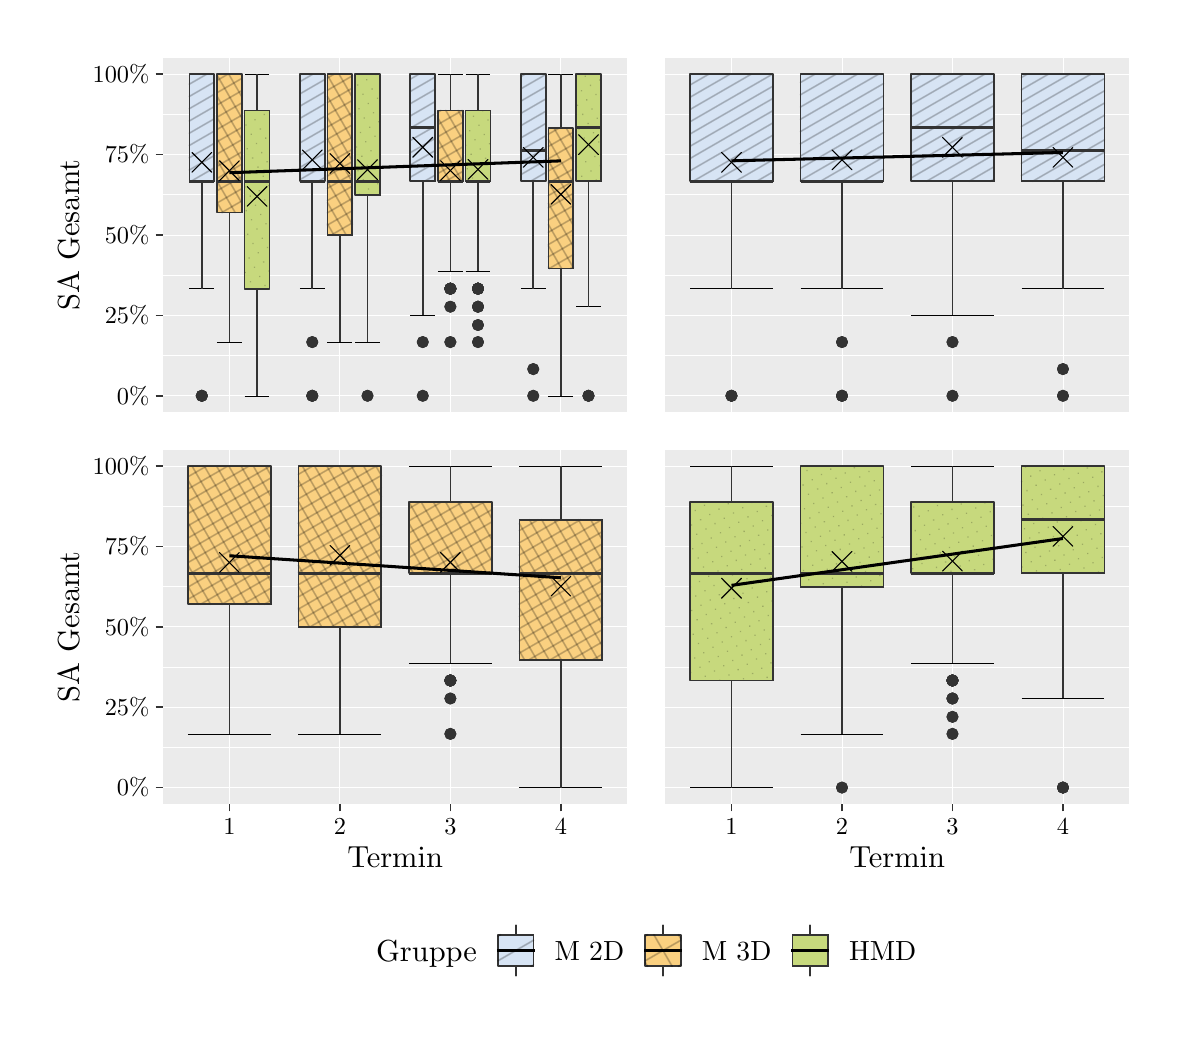
\begin{tikzpicture}[x=1pt,y=1pt]
\definecolor{fillColor}{RGB}{255,255,255}
\path[use as bounding box,fill=fillColor,fill opacity=0.00] (0,0) rectangle (409.05,361.35);
\begin{scope}
\path[clip] (  0.00,  0.00) rectangle (409.05,361.35);
\definecolor{drawColor}{RGB}{255,255,255}
\definecolor{fillColor}{RGB}{255,255,255}

\path[draw=drawColor,line width= 0.6pt,line join=round,line cap=round,fill=fillColor] (  0.00,  0.00) rectangle (409.05,361.35);
\end{scope}
\begin{scope}
\path[clip] (  5.50,214.27) rectangle (222.12,355.85);
\definecolor{drawColor}{RGB}{255,255,255}
\definecolor{fillColor}{RGB}{255,255,255}

\path[draw=drawColor,line width= 0.6pt,line join=round,line cap=round,fill=fillColor] (  5.50,214.27) rectangle (222.12,355.85);
\end{scope}
\begin{scope}
\path[clip] ( 48.94,222.52) rectangle (216.62,350.35);
\definecolor{fillColor}{gray}{0.92}

\path[fill=fillColor] ( 48.94,222.52) rectangle (216.62,350.35);
\definecolor{drawColor}{RGB}{255,255,255}

\path[draw=drawColor,line width= 0.3pt,line join=round] ( 48.94,242.86) --
	(216.62,242.86);

\path[draw=drawColor,line width= 0.3pt,line join=round] ( 48.94,271.91) --
	(216.62,271.91);

\path[draw=drawColor,line width= 0.3pt,line join=round] ( 48.94,300.96) --
	(216.62,300.96);

\path[draw=drawColor,line width= 0.3pt,line join=round] ( 48.94,330.01) --
	(216.62,330.01);

\path[draw=drawColor,line width= 0.3pt,line join=round] ( 48.94,228.33) --
	(216.62,228.33);

\path[draw=drawColor,line width= 0.3pt,line join=round] ( 48.94,257.39) --
	(216.62,257.39);

\path[draw=drawColor,line width= 0.3pt,line join=round] ( 48.94,286.44) --
	(216.62,286.44);

\path[draw=drawColor,line width= 0.3pt,line join=round] ( 48.94,315.49) --
	(216.62,315.49);

\path[draw=drawColor,line width= 0.3pt,line join=round] ( 48.94,344.54) --
	(216.62,344.54);

\path[draw=drawColor,line width= 0.3pt,line join=round] ( 72.90,222.52) --
	( 72.90,350.35);

\path[draw=drawColor,line width= 0.3pt,line join=round] (112.82,222.52) --
	(112.82,350.35);

\path[draw=drawColor,line width= 0.3pt,line join=round] (152.74,222.52) --
	(152.74,350.35);

\path[draw=drawColor,line width= 0.3pt,line join=round] (192.67,222.52) --
	(192.67,350.35);
\definecolor{drawColor}{RGB}{0,0,0}

\path[draw=drawColor,line width= 0.2pt,line join=round] ( 58.42,344.54) --
	( 67.41,344.54);

\path[draw=drawColor,line width= 0.2pt,line join=round] ( 62.92,344.54) --
	( 62.92,267.03);

\path[draw=drawColor,line width= 0.2pt,line join=round] ( 58.42,267.03) --
	( 67.41,267.03);

\path[draw=drawColor,line width= 0.2pt,line join=round] ( 68.41,344.54) --
	( 77.39,344.54);

\path[draw=drawColor,line width= 0.2pt,line join=round] ( 72.90,344.54) --
	( 72.90,247.74);

\path[draw=drawColor,line width= 0.2pt,line join=round] ( 68.41,247.74) --
	( 77.39,247.74);

\path[draw=drawColor,line width= 0.2pt,line join=round] ( 78.39,344.54) --
	( 87.37,344.54);

\path[draw=drawColor,line width= 0.2pt,line join=round] ( 82.88,344.54) --
	( 82.88,228.33);

\path[draw=drawColor,line width= 0.2pt,line join=round] ( 78.39,228.33) --
	( 87.37,228.33);

\path[draw=drawColor,line width= 0.2pt,line join=round] ( 98.35,344.54) --
	(107.33,344.54);

\path[draw=drawColor,line width= 0.2pt,line join=round] (102.84,344.54) --
	(102.84,267.03);

\path[draw=drawColor,line width= 0.2pt,line join=round] ( 98.35,267.03) --
	(107.33,267.03);

\path[draw=drawColor,line width= 0.2pt,line join=round] (108.33,344.54) --
	(117.31,344.54);

\path[draw=drawColor,line width= 0.2pt,line join=round] (112.82,344.54) --
	(112.82,247.74);

\path[draw=drawColor,line width= 0.2pt,line join=round] (108.33,247.74) --
	(117.31,247.74);

\path[draw=drawColor,line width= 0.2pt,line join=round] (118.31,344.54) --
	(127.29,344.54);

\path[draw=drawColor,line width= 0.2pt,line join=round] (122.80,344.54) --
	(122.80,247.74);

\path[draw=drawColor,line width= 0.2pt,line join=round] (118.31,247.74) --
	(127.29,247.74);

\path[draw=drawColor,line width= 0.2pt,line join=round] (138.27,344.54) --
	(147.25,344.54);

\path[draw=drawColor,line width= 0.2pt,line join=round] (142.76,344.54) --
	(142.76,257.39);

\path[draw=drawColor,line width= 0.2pt,line join=round] (138.27,257.39) --
	(147.25,257.39);

\path[draw=drawColor,line width= 0.2pt,line join=round] (148.25,344.54) --
	(157.23,344.54);

\path[draw=drawColor,line width= 0.2pt,line join=round] (152.74,344.54) --
	(152.74,273.31);

\path[draw=drawColor,line width= 0.2pt,line join=round] (148.25,273.31) --
	(157.23,273.31);

\path[draw=drawColor,line width= 0.2pt,line join=round] (158.23,344.54) --
	(167.22,344.54);

\path[draw=drawColor,line width= 0.2pt,line join=round] (162.72,344.54) --
	(162.72,273.31);

\path[draw=drawColor,line width= 0.2pt,line join=round] (158.23,273.31) --
	(167.22,273.31);

\path[draw=drawColor,line width= 0.2pt,line join=round] (178.19,344.54) --
	(187.18,344.54);

\path[draw=drawColor,line width= 0.2pt,line join=round] (182.69,344.54) --
	(182.69,267.03);

\path[draw=drawColor,line width= 0.2pt,line join=round] (178.19,267.03) --
	(187.18,267.03);

\path[draw=drawColor,line width= 0.2pt,line join=round] (188.18,344.54) --
	(197.16,344.54);

\path[draw=drawColor,line width= 0.2pt,line join=round] (192.67,344.54) --
	(192.67,228.33);

\path[draw=drawColor,line width= 0.2pt,line join=round] (188.18,228.33) --
	(197.16,228.33);

\path[draw=drawColor,line width= 0.2pt,line join=round] (198.16,344.54) --
	(207.14,344.54);

\path[draw=drawColor,line width= 0.2pt,line join=round] (202.65,344.54) --
	(202.65,260.52);

\path[draw=drawColor,line width= 0.2pt,line join=round] (198.16,260.52) --
	(207.14,260.52);
\definecolor{drawColor}{gray}{0.20}
\definecolor{fillColor}{gray}{0.20}

\path[draw=drawColor,line width= 0.4pt,line join=round,line cap=round,fill=fillColor] ( 62.92,228.33) circle (  1.96);

\path[draw=drawColor,line width= 0.4pt,line join=round,line cap=round,fill=fillColor] ( 62.92,228.33) circle (  1.96);

\path[draw=drawColor,line width= 0.2pt,line join=round] ( 62.92,344.54) -- ( 62.92,344.54);

\path[draw=drawColor,line width= 0.2pt,line join=round] ( 62.92,305.84) -- ( 62.92,267.03);
\definecolor{fillColor}{RGB}{215,228,244}

\path[draw=drawColor,line width= 0.2pt,fill=fillColor] ( 58.42,344.54) --
	( 58.42,305.84) --
	( 67.41,305.84) --
	( 67.41,344.54) --
	( 58.42,344.54) --
	cycle;

\path[draw=drawColor,line width= 0.5pt] ( 58.42,305.84) -- ( 67.41,305.84);

\path[draw=drawColor,line width= 0.2pt,line join=round] ( 72.90,344.54) -- ( 72.90,344.54);

\path[draw=drawColor,line width= 0.2pt,line join=round] ( 72.90,294.57) -- ( 72.90,247.74);
\definecolor{fillColor}{RGB}{250,208,128}

\path[draw=drawColor,line width= 0.2pt,fill=fillColor] ( 68.41,344.54) --
	( 68.41,294.57) --
	( 77.39,294.57) --
	( 77.39,344.54) --
	( 68.41,344.54) --
	cycle;

\path[draw=drawColor,line width= 0.5pt] ( 68.41,305.84) -- ( 77.39,305.84);

\path[draw=drawColor,line width= 0.2pt,line join=round] ( 82.88,331.41) -- ( 82.88,344.54);

\path[draw=drawColor,line width= 0.2pt,line join=round] ( 82.88,267.03) -- ( 82.88,228.33);
\definecolor{fillColor}{RGB}{199,217,125}

\path[draw=drawColor,line width= 0.2pt,fill=fillColor] ( 78.39,331.41) --
	( 78.39,267.03) --
	( 87.37,267.03) --
	( 87.37,331.41) --
	( 78.39,331.41) --
	cycle;

\path[draw=drawColor,line width= 0.5pt] ( 78.39,305.84) -- ( 87.37,305.84);
\definecolor{fillColor}{gray}{0.20}

\path[draw=drawColor,line width= 0.4pt,line join=round,line cap=round,fill=fillColor] (102.84,228.33) circle (  1.96);

\path[draw=drawColor,line width= 0.4pt,line join=round,line cap=round,fill=fillColor] (102.84,247.74) circle (  1.96);

\path[draw=drawColor,line width= 0.4pt,line join=round,line cap=round,fill=fillColor] (102.84,228.33) circle (  1.96);

\path[draw=drawColor,line width= 0.2pt,line join=round] (102.84,344.54) -- (102.84,344.54);

\path[draw=drawColor,line width= 0.2pt,line join=round] (102.84,305.84) -- (102.84,267.03);
\definecolor{fillColor}{RGB}{215,228,244}

\path[draw=drawColor,line width= 0.2pt,fill=fillColor] ( 98.35,344.54) --
	( 98.35,305.84) --
	(107.33,305.84) --
	(107.33,344.54) --
	( 98.35,344.54) --
	cycle;

\path[draw=drawColor,line width= 0.5pt] ( 98.35,305.84) -- (107.33,305.84);

\path[draw=drawColor,line width= 0.2pt,line join=round] (112.82,344.54) -- (112.82,344.54);

\path[draw=drawColor,line width= 0.2pt,line join=round] (112.82,286.44) -- (112.82,247.74);
\definecolor{fillColor}{RGB}{250,208,128}

\path[draw=drawColor,line width= 0.2pt,fill=fillColor] (108.33,344.54) --
	(108.33,286.44) --
	(117.31,286.44) --
	(117.31,344.54) --
	(108.33,344.54) --
	cycle;

\path[draw=drawColor,line width= 0.5pt] (108.33,305.84) -- (117.31,305.84);
\definecolor{fillColor}{gray}{0.20}

\path[draw=drawColor,line width= 0.4pt,line join=round,line cap=round,fill=fillColor] (122.80,228.33) circle (  1.96);

\path[draw=drawColor,line width= 0.2pt,line join=round] (122.80,344.54) -- (122.80,344.54);

\path[draw=drawColor,line width= 0.2pt,line join=round] (122.80,300.88) -- (122.80,247.74);
\definecolor{fillColor}{RGB}{199,217,125}

\path[draw=drawColor,line width= 0.2pt,fill=fillColor] (118.31,344.54) --
	(118.31,300.88) --
	(127.29,300.88) --
	(127.29,344.54) --
	(118.31,344.54) --
	cycle;

\path[draw=drawColor,line width= 0.5pt] (118.31,305.84) -- (127.29,305.84);
\definecolor{fillColor}{gray}{0.20}

\path[draw=drawColor,line width= 0.4pt,line join=round,line cap=round,fill=fillColor] (142.76,228.33) circle (  1.96);

\path[draw=drawColor,line width= 0.4pt,line join=round,line cap=round,fill=fillColor] (142.76,247.74) circle (  1.96);

\path[draw=drawColor,line width= 0.2pt,line join=round] (142.76,344.54) -- (142.76,344.54);

\path[draw=drawColor,line width= 0.2pt,line join=round] (142.76,305.84) -- (142.76,257.39);
\definecolor{fillColor}{RGB}{215,228,244}

\path[draw=drawColor,line width= 0.2pt,fill=fillColor] (138.27,344.54) --
	(138.27,305.84) --
	(147.25,305.84) --
	(147.25,344.54) --
	(138.27,344.54) --
	cycle;

\path[draw=drawColor,line width= 0.5pt] (138.27,325.13) -- (147.25,325.13);
\definecolor{fillColor}{gray}{0.20}

\path[draw=drawColor,line width= 0.4pt,line join=round,line cap=round,fill=fillColor] (152.74,267.03) circle (  1.96);

\path[draw=drawColor,line width= 0.4pt,line join=round,line cap=round,fill=fillColor] (152.74,267.03) circle (  1.96);

\path[draw=drawColor,line width= 0.4pt,line join=round,line cap=round,fill=fillColor] (152.74,267.03) circle (  1.96);

\path[draw=drawColor,line width= 0.4pt,line join=round,line cap=round,fill=fillColor] (152.74,267.03) circle (  1.96);

\path[draw=drawColor,line width= 0.4pt,line join=round,line cap=round,fill=fillColor] (152.74,260.52) circle (  1.96);

\path[draw=drawColor,line width= 0.4pt,line join=round,line cap=round,fill=fillColor] (152.74,247.74) circle (  1.96);

\path[draw=drawColor,line width= 0.4pt,line join=round,line cap=round,fill=fillColor] (152.74,267.03) circle (  1.96);

\path[draw=drawColor,line width= 0.2pt,line join=round] (152.74,331.41) -- (152.74,344.54);

\path[draw=drawColor,line width= 0.2pt,line join=round] (152.74,305.84) -- (152.74,273.31);
\definecolor{fillColor}{RGB}{250,208,128}

\path[draw=drawColor,line width= 0.2pt,fill=fillColor] (148.25,331.41) --
	(148.25,305.84) --
	(157.23,305.84) --
	(157.23,331.41) --
	(148.25,331.41) --
	cycle;

\path[draw=drawColor,line width= 0.5pt] (148.25,305.84) -- (157.23,305.84);
\definecolor{fillColor}{gray}{0.20}

\path[draw=drawColor,line width= 0.4pt,line join=round,line cap=round,fill=fillColor] (162.72,267.03) circle (  1.96);

\path[draw=drawColor,line width= 0.4pt,line join=round,line cap=round,fill=fillColor] (162.72,267.03) circle (  1.96);

\path[draw=drawColor,line width= 0.4pt,line join=round,line cap=round,fill=fillColor] (162.72,267.03) circle (  1.96);

\path[draw=drawColor,line width= 0.4pt,line join=round,line cap=round,fill=fillColor] (162.72,260.52) circle (  1.96);

\path[draw=drawColor,line width= 0.4pt,line join=round,line cap=round,fill=fillColor] (162.72,253.90) circle (  1.96);

\path[draw=drawColor,line width= 0.4pt,line join=round,line cap=round,fill=fillColor] (162.72,267.03) circle (  1.96);

\path[draw=drawColor,line width= 0.4pt,line join=round,line cap=round,fill=fillColor] (162.72,260.52) circle (  1.96);

\path[draw=drawColor,line width= 0.4pt,line join=round,line cap=round,fill=fillColor] (162.72,247.74) circle (  1.96);

\path[draw=drawColor,line width= 0.4pt,line join=round,line cap=round,fill=fillColor] (162.72,267.03) circle (  1.96);

\path[draw=drawColor,line width= 0.2pt,line join=round] (162.72,331.41) -- (162.72,344.54);

\path[draw=drawColor,line width= 0.2pt,line join=round] (162.72,305.84) -- (162.72,273.31);
\definecolor{fillColor}{RGB}{199,217,125}

\path[draw=drawColor,line width= 0.2pt,fill=fillColor] (158.23,331.41) --
	(158.23,305.84) --
	(167.22,305.84) --
	(167.22,331.41) --
	(158.23,331.41) --
	cycle;

\path[draw=drawColor,line width= 0.5pt] (158.23,305.84) -- (167.22,305.84);
\definecolor{fillColor}{gray}{0.20}

\path[draw=drawColor,line width= 0.4pt,line join=round,line cap=round,fill=fillColor] (182.69,228.33) circle (  1.96);

\path[draw=drawColor,line width= 0.4pt,line join=round,line cap=round,fill=fillColor] (182.69,237.98) circle (  1.96);

\path[draw=drawColor,line width= 0.2pt,line join=round] (182.69,344.54) -- (182.69,344.54);

\path[draw=drawColor,line width= 0.2pt,line join=round] (182.69,305.84) -- (182.69,267.03);
\definecolor{fillColor}{RGB}{215,228,244}

\path[draw=drawColor,line width= 0.2pt,fill=fillColor] (178.19,344.54) --
	(178.19,305.84) --
	(187.18,305.84) --
	(187.18,344.54) --
	(178.19,344.54) --
	cycle;

\path[draw=drawColor,line width= 0.5pt] (178.19,317.00) -- (187.18,317.00);

\path[draw=drawColor,line width= 0.2pt,line join=round] (192.67,325.13) -- (192.67,344.54);

\path[draw=drawColor,line width= 0.2pt,line join=round] (192.67,274.35) -- (192.67,228.33);
\definecolor{fillColor}{RGB}{250,208,128}

\path[draw=drawColor,line width= 0.2pt,fill=fillColor] (188.18,325.13) --
	(188.18,274.35) --
	(197.16,274.35) --
	(197.16,325.13) --
	(188.18,325.13) --
	cycle;

\path[draw=drawColor,line width= 0.5pt] (188.18,305.84) -- (197.16,305.84);
\definecolor{fillColor}{gray}{0.20}

\path[draw=drawColor,line width= 0.4pt,line join=round,line cap=round,fill=fillColor] (202.65,228.33) circle (  1.96);

\path[draw=drawColor,line width= 0.4pt,line join=round,line cap=round,fill=fillColor] (202.65,228.33) circle (  1.96);

\path[draw=drawColor,line width= 0.2pt,line join=round] (202.65,344.54) -- (202.65,344.54);

\path[draw=drawColor,line width= 0.2pt,line join=round] (202.65,305.84) -- (202.65,260.52);
\definecolor{fillColor}{RGB}{199,217,125}

\path[draw=drawColor,line width= 0.2pt,fill=fillColor] (198.16,344.54) --
	(198.16,305.84) --
	(207.14,305.84) --
	(207.14,344.54) --
	(198.16,344.54) --
	cycle;

\path[draw=drawColor,line width= 0.5pt] (198.16,325.13) -- (207.14,325.13);
\definecolor{fillColor}{gray}{0.20}

\path[draw=drawColor,line width= 0.4pt,line join=round,line cap=round,fill=fillColor] ( 62.92,228.33) circle (  1.96);

\path[draw=drawColor,line width= 0.4pt,line join=round,line cap=round,fill=fillColor] ( 62.92,228.33) circle (  1.96);

\path[draw=drawColor,line width= 0.6pt,line join=round] ( 62.92,344.54) -- ( 62.92,344.54);

\path[draw=drawColor,line width= 0.6pt,line join=round] ( 62.92,305.84) -- ( 62.92,267.03);
\definecolor{fillColor}{RGB}{215,228,244}

\path[fill=fillColor] ( 58.42,344.54) --
	( 58.42,305.84) --
	( 67.41,305.84) --
	( 67.41,344.54) --
	( 58.42,344.54) --
	cycle;
\definecolor{drawColor}{RGB}{0,0,0}
\definecolor{fillColor}{RGB}{0,0,0}

\path[draw=drawColor,draw opacity=0.20,line width= 0.6pt,line join=round,line cap=rect,fill=fillColor,fill opacity=0.20] ( 67.41,306.28) --
	( 67.41,306.24) --
	( 66.73,305.84) --
	( 66.65,305.84) --
	( 67.41,306.28) --
	cycle;

\path[draw=drawColor,draw opacity=0.20,line width= 0.6pt,line join=round,line cap=rect,fill=fillColor,fill opacity=0.20] ( 67.41,310.71) --
	( 67.41,310.66) --
	( 59.06,305.84) --
	( 58.98,305.84) --
	( 67.41,310.71) --
	cycle;

\path[draw=drawColor,draw opacity=0.20,line width= 0.6pt,line join=round,line cap=rect,fill=fillColor,fill opacity=0.20] ( 67.41,315.14) --
	( 67.41,315.09) --
	( 58.42,309.91) --
	( 58.42,309.95) --
	( 67.41,315.14) --
	cycle;

\path[draw=drawColor,draw opacity=0.20,line width= 0.6pt,line join=round,line cap=rect,fill=fillColor,fill opacity=0.20] ( 67.41,319.56) --
	( 67.41,319.52) --
	( 58.42,314.33) --
	( 58.42,314.38) --
	( 67.41,319.56) --
	cycle;

\path[draw=drawColor,draw opacity=0.20,line width= 0.6pt,line join=round,line cap=rect,fill=fillColor,fill opacity=0.20] ( 67.41,323.99) --
	( 67.41,323.95) --
	( 58.42,318.76) --
	( 58.42,318.81) --
	( 67.41,323.99) --
	cycle;

\path[draw=drawColor,draw opacity=0.20,line width= 0.6pt,line join=round,line cap=rect,fill=fillColor,fill opacity=0.20] ( 67.41,328.42) --
	( 67.41,328.38) --
	( 58.42,323.19) --
	( 58.42,323.23) --
	( 67.41,328.42) --
	cycle;

\path[draw=drawColor,draw opacity=0.20,line width= 0.6pt,line join=round,line cap=rect,fill=fillColor,fill opacity=0.20] ( 67.41,332.85) --
	( 67.41,332.80) --
	( 58.42,327.62) --
	( 58.42,327.66) --
	( 67.41,332.85) --
	cycle;

\path[draw=drawColor,draw opacity=0.20,line width= 0.6pt,line join=round,line cap=rect,fill=fillColor,fill opacity=0.20] ( 67.41,337.28) --
	( 67.41,337.23) --
	( 58.42,332.05) --
	( 58.42,332.09) --
	( 67.41,337.28) --
	cycle;

\path[draw=drawColor,draw opacity=0.20,line width= 0.6pt,line join=round,line cap=rect,fill=fillColor,fill opacity=0.20] ( 67.41,341.70) --
	( 67.41,341.66) --
	( 58.42,336.47) --
	( 58.42,336.52) --
	( 67.41,341.70) --
	cycle;

\path[draw=drawColor,draw opacity=0.20,line width= 0.6pt,line join=round,line cap=rect,fill=fillColor,fill opacity=0.20] ( 64.65,344.54) --
	( 64.73,344.54) --
	( 58.42,340.90) --
	( 58.42,340.95) --
	( 64.65,344.54) --
	cycle;
\definecolor{drawColor}{gray}{0.20}

\path[draw=drawColor,line width= 0.6pt,line join=round,line cap=round] ( 58.42,344.54) --
	( 58.42,305.84) --
	( 67.41,305.84) --
	( 67.41,344.54) --
	( 58.42,344.54) --
	cycle;

\path[draw=drawColor,line width= 1.1pt,line join=round] ( 58.42,305.84) -- ( 67.41,305.84);
\definecolor{fillColor}{gray}{0.20}

\path[draw=drawColor,line width= 0.4pt,line join=round,line cap=round,fill=fillColor] (102.84,228.33) circle (  1.96);

\path[draw=drawColor,line width= 0.4pt,line join=round,line cap=round,fill=fillColor] (102.84,247.74) circle (  1.96);

\path[draw=drawColor,line width= 0.4pt,line join=round,line cap=round,fill=fillColor] (102.84,228.33) circle (  1.96);

\path[draw=drawColor,line width= 0.6pt,line join=round] (102.84,344.54) -- (102.84,344.54);

\path[draw=drawColor,line width= 0.6pt,line join=round] (102.84,305.84) -- (102.84,267.03);
\definecolor{fillColor}{RGB}{215,228,244}

\path[fill=fillColor] ( 98.35,344.54) --
	( 98.35,305.84) --
	(107.33,305.84) --
	(107.33,344.54) --
	( 98.35,344.54) --
	cycle;
\definecolor{drawColor}{RGB}{0,0,0}
\definecolor{fillColor}{RGB}{0,0,0}

\path[draw=drawColor,draw opacity=0.20,line width= 0.6pt,line join=round,line cap=rect,fill=fillColor,fill opacity=0.20] (107.33,307.19) --
	(107.33,307.14) --
	(105.08,305.84) --
	(105.00,305.84) --
	(107.33,307.19) --
	cycle;

\path[draw=drawColor,draw opacity=0.20,line width= 0.6pt,line join=round,line cap=rect,fill=fillColor,fill opacity=0.20] (107.33,311.62) --
	(107.33,311.57) --
	( 98.35,306.39) --
	( 98.35,306.43) --
	(107.33,311.62) --
	cycle;

\path[draw=drawColor,draw opacity=0.20,line width= 0.6pt,line join=round,line cap=rect,fill=fillColor,fill opacity=0.20] (107.33,316.05) --
	(107.33,316.00) --
	( 98.35,310.81) --
	( 98.35,310.86) --
	(107.33,316.05) --
	cycle;

\path[draw=drawColor,draw opacity=0.20,line width= 0.6pt,line join=round,line cap=rect,fill=fillColor,fill opacity=0.20] (107.33,320.47) --
	(107.33,320.43) --
	( 98.35,315.24) --
	( 98.35,315.29) --
	(107.33,320.47) --
	cycle;

\path[draw=drawColor,draw opacity=0.20,line width= 0.6pt,line join=round,line cap=rect,fill=fillColor,fill opacity=0.20] (107.33,324.90) --
	(107.33,324.86) --
	( 98.35,319.67) --
	( 98.35,319.72) --
	(107.33,324.90) --
	cycle;

\path[draw=drawColor,draw opacity=0.20,line width= 0.6pt,line join=round,line cap=rect,fill=fillColor,fill opacity=0.20] (107.33,329.33) --
	(107.33,329.28) --
	( 98.35,324.10) --
	( 98.35,324.14) --
	(107.33,329.33) --
	cycle;

\path[draw=drawColor,draw opacity=0.20,line width= 0.6pt,line join=round,line cap=rect,fill=fillColor,fill opacity=0.20] (107.33,333.76) --
	(107.33,333.71) --
	( 98.35,328.53) --
	( 98.35,328.57) --
	(107.33,333.76) --
	cycle;

\path[draw=drawColor,draw opacity=0.20,line width= 0.6pt,line join=round,line cap=rect,fill=fillColor,fill opacity=0.20] (107.33,338.19) --
	(107.33,338.14) --
	( 98.35,332.95) --
	( 98.35,333.00) --
	(107.33,338.19) --
	cycle;

\path[draw=drawColor,draw opacity=0.20,line width= 0.6pt,line join=round,line cap=rect,fill=fillColor,fill opacity=0.20] (107.33,342.61) --
	(107.33,342.57) --
	( 98.35,337.38) --
	( 98.35,337.43) --
	(107.33,342.61) --
	cycle;

\path[draw=drawColor,draw opacity=0.20,line width= 0.6pt,line join=round,line cap=rect,fill=fillColor,fill opacity=0.20] (103.00,344.54) --
	(103.07,344.54) --
	( 98.35,341.81) --
	( 98.35,341.86) --
	(103.00,344.54) --
	cycle;
\definecolor{drawColor}{gray}{0.20}

\path[draw=drawColor,line width= 0.6pt,line join=round,line cap=round] ( 98.35,344.54) --
	( 98.35,305.84) --
	(107.33,305.84) --
	(107.33,344.54) --
	( 98.35,344.54) --
	cycle;

\path[draw=drawColor,line width= 1.1pt,line join=round] ( 98.35,305.84) -- (107.33,305.84);
\definecolor{fillColor}{gray}{0.20}

\path[draw=drawColor,line width= 0.4pt,line join=round,line cap=round,fill=fillColor] (142.76,228.33) circle (  1.96);

\path[draw=drawColor,line width= 0.4pt,line join=round,line cap=round,fill=fillColor] (142.76,247.74) circle (  1.96);

\path[draw=drawColor,line width= 0.6pt,line join=round] (142.76,344.54) -- (142.76,344.54);

\path[draw=drawColor,line width= 0.6pt,line join=round] (142.76,305.84) -- (142.76,257.39);
\definecolor{fillColor}{RGB}{215,228,244}

\path[fill=fillColor] (138.27,344.54) --
	(138.27,305.84) --
	(147.25,305.84) --
	(147.25,344.54) --
	(138.27,344.54) --
	cycle;
\definecolor{drawColor}{RGB}{0,0,0}
\definecolor{fillColor}{RGB}{0,0,0}

\path[draw=drawColor,draw opacity=0.20,line width= 0.6pt,line join=round,line cap=rect,fill=fillColor,fill opacity=0.20] (147.25,308.10) --
	(147.25,308.05) --
	(143.42,305.84) --
	(143.35,305.84) --
	(147.25,308.10) --
	cycle;

\path[draw=drawColor,draw opacity=0.20,line width= 0.6pt,line join=round,line cap=rect,fill=fillColor,fill opacity=0.20] (147.25,312.53) --
	(147.25,312.48) --
	(138.27,307.30) --
	(138.27,307.34) --
	(147.25,312.53) --
	cycle;

\path[draw=drawColor,draw opacity=0.20,line width= 0.6pt,line join=round,line cap=rect,fill=fillColor,fill opacity=0.20] (147.25,316.95) --
	(147.25,316.91) --
	(138.27,311.72) --
	(138.27,311.77) --
	(147.25,316.95) --
	cycle;

\path[draw=drawColor,draw opacity=0.20,line width= 0.6pt,line join=round,line cap=rect,fill=fillColor,fill opacity=0.20] (147.25,321.38) --
	(147.25,321.34) --
	(138.27,316.15) --
	(138.27,316.20) --
	(147.25,321.38) --
	cycle;

\path[draw=drawColor,draw opacity=0.20,line width= 0.6pt,line join=round,line cap=rect,fill=fillColor,fill opacity=0.20] (147.25,325.81) --
	(147.25,325.77) --
	(138.27,320.58) --
	(138.27,320.62) --
	(147.25,325.81) --
	cycle;

\path[draw=drawColor,draw opacity=0.20,line width= 0.6pt,line join=round,line cap=rect,fill=fillColor,fill opacity=0.20] (147.25,330.24) --
	(147.25,330.19) --
	(138.27,325.01) --
	(138.27,325.05) --
	(147.25,330.24) --
	cycle;

\path[draw=drawColor,draw opacity=0.20,line width= 0.6pt,line join=round,line cap=rect,fill=fillColor,fill opacity=0.20] (147.25,334.67) --
	(147.25,334.62) --
	(138.27,329.44) --
	(138.27,329.48) --
	(147.25,334.67) --
	cycle;

\path[draw=drawColor,draw opacity=0.20,line width= 0.6pt,line join=round,line cap=rect,fill=fillColor,fill opacity=0.20] (147.25,339.09) --
	(147.25,339.05) --
	(138.27,333.86) --
	(138.27,333.91) --
	(147.25,339.09) --
	cycle;

\path[draw=drawColor,draw opacity=0.20,line width= 0.6pt,line join=round,line cap=rect,fill=fillColor,fill opacity=0.20] (147.25,343.52) --
	(147.25,343.48) --
	(138.27,338.29) --
	(138.27,338.34) --
	(147.25,343.52) --
	cycle;

\path[draw=drawColor,draw opacity=0.20,line width= 0.6pt,line join=round,line cap=rect,fill=fillColor,fill opacity=0.20] (141.35,344.54) --
	(141.42,344.54) --
	(138.27,342.72) --
	(138.27,342.76) --
	(141.35,344.54) --
	cycle;
\definecolor{drawColor}{gray}{0.20}

\path[draw=drawColor,line width= 0.6pt,line join=round,line cap=round] (138.27,344.54) --
	(138.27,305.84) --
	(147.25,305.84) --
	(147.25,344.54) --
	(138.27,344.54) --
	cycle;

\path[draw=drawColor,line width= 1.1pt,line join=round] (138.27,325.13) -- (147.25,325.13);
\definecolor{fillColor}{gray}{0.20}

\path[draw=drawColor,line width= 0.4pt,line join=round,line cap=round,fill=fillColor] (182.69,228.33) circle (  1.96);

\path[draw=drawColor,line width= 0.4pt,line join=round,line cap=round,fill=fillColor] (182.69,237.98) circle (  1.96);

\path[draw=drawColor,line width= 0.6pt,line join=round] (182.69,344.54) -- (182.69,344.54);

\path[draw=drawColor,line width= 0.6pt,line join=round] (182.69,305.84) -- (182.69,267.03);
\definecolor{fillColor}{RGB}{215,228,244}

\path[fill=fillColor] (178.19,344.54) --
	(178.19,305.84) --
	(187.18,305.84) --
	(187.18,344.54) --
	(178.19,344.54) --
	cycle;
\definecolor{drawColor}{RGB}{0,0,0}
\definecolor{fillColor}{RGB}{0,0,0}

\path[draw=drawColor,draw opacity=0.20,line width= 0.6pt,line join=round,line cap=rect,fill=fillColor,fill opacity=0.20] (187.18,309.01) --
	(187.18,308.96) --
	(181.77,305.84) --
	(181.70,305.84) --
	(187.18,309.01) --
	cycle;

\path[draw=drawColor,draw opacity=0.20,line width= 0.6pt,line join=round,line cap=rect,fill=fillColor,fill opacity=0.20] (187.18,313.44) --
	(187.18,313.39) --
	(178.19,308.21) --
	(178.19,308.25) --
	(187.18,313.44) --
	cycle;

\path[draw=drawColor,draw opacity=0.20,line width= 0.6pt,line join=round,line cap=rect,fill=fillColor,fill opacity=0.20] (187.18,317.86) --
	(187.18,317.82) --
	(178.19,312.63) --
	(178.19,312.68) --
	(187.18,317.86) --
	cycle;

\path[draw=drawColor,draw opacity=0.20,line width= 0.6pt,line join=round,line cap=rect,fill=fillColor,fill opacity=0.20] (187.18,322.29) --
	(187.18,322.25) --
	(178.19,317.06) --
	(178.19,317.11) --
	(187.18,322.29) --
	cycle;

\path[draw=drawColor,draw opacity=0.20,line width= 0.6pt,line join=round,line cap=rect,fill=fillColor,fill opacity=0.20] (187.18,326.72) --
	(187.18,326.68) --
	(178.19,321.49) --
	(178.19,321.53) --
	(187.18,326.72) --
	cycle;

\path[draw=drawColor,draw opacity=0.20,line width= 0.6pt,line join=round,line cap=rect,fill=fillColor,fill opacity=0.20] (187.18,331.15) --
	(187.18,331.10) --
	(178.19,325.92) --
	(178.19,325.96) --
	(187.18,331.15) --
	cycle;

\path[draw=drawColor,draw opacity=0.20,line width= 0.6pt,line join=round,line cap=rect,fill=fillColor,fill opacity=0.20] (187.18,335.58) --
	(187.18,335.53) --
	(178.19,330.35) --
	(178.19,330.39) --
	(187.18,335.58) --
	cycle;

\path[draw=drawColor,draw opacity=0.20,line width= 0.6pt,line join=round,line cap=rect,fill=fillColor,fill opacity=0.20] (187.18,340.00) --
	(187.18,339.96) --
	(178.19,334.77) --
	(178.19,334.82) --
	(187.18,340.00) --
	cycle;

\path[draw=drawColor,draw opacity=0.20,line width= 0.6pt,line join=round,line cap=rect,fill=fillColor,fill opacity=0.20] (187.18,344.43) --
	(187.18,344.39) --
	(178.19,339.20) --
	(178.19,339.25) --
	(187.18,344.43) --
	cycle;

\path[draw=drawColor,draw opacity=0.20,line width= 0.6pt,line join=round,line cap=rect,fill=fillColor,fill opacity=0.20] (179.69,344.54) --
	(179.77,344.54) --
	(178.19,343.63) --
	(178.19,343.67) --
	(179.69,344.54) --
	cycle;
\definecolor{drawColor}{gray}{0.20}

\path[draw=drawColor,line width= 0.6pt,line join=round,line cap=round] (178.19,344.54) --
	(178.19,305.84) --
	(187.18,305.84) --
	(187.18,344.54) --
	(178.19,344.54) --
	cycle;

\path[draw=drawColor,line width= 1.1pt,line join=round] (178.19,317.00) -- (187.18,317.00);

\path[draw=drawColor,line width= 0.6pt,line join=round] ( 72.90,344.54) -- ( 72.90,344.54);

\path[draw=drawColor,line width= 0.6pt,line join=round] ( 72.90,294.57) -- ( 72.90,247.74);
\definecolor{fillColor}{RGB}{250,208,128}

\path[fill=fillColor] ( 68.41,344.54) --
	( 68.41,294.57) --
	( 77.39,294.57) --
	( 77.39,344.54) --
	( 68.41,344.54) --
	cycle;
\definecolor{drawColor}{RGB}{0,0,0}
\definecolor{fillColor}{RGB}{0,0,0}

\path[draw=drawColor,draw opacity=0.20,line width= 0.6pt,line join=round,line cap=rect,fill=fillColor,fill opacity=0.20] ( 77.39,298.76) --
	( 77.39,298.71) --
	( 70.21,294.57) --
	( 70.14,294.57) --
	( 77.39,298.76) --
	cycle;

\path[draw=drawColor,draw opacity=0.20,line width= 0.6pt,line join=round,line cap=rect,fill=fillColor,fill opacity=0.20] ( 77.39,303.19) --
	( 77.39,303.14) --
	( 68.41,297.96) --
	( 68.41,298.00) --
	( 77.39,303.19) --
	cycle;

\path[draw=drawColor,draw opacity=0.20,line width= 0.6pt,line join=round,line cap=rect,fill=fillColor,fill opacity=0.20] ( 77.39,307.61) --
	( 77.39,307.57) --
	( 68.41,302.38) --
	( 68.41,302.43) --
	( 77.39,307.61) --
	cycle;

\path[draw=drawColor,draw opacity=0.20,line width= 0.6pt,line join=round,line cap=rect,fill=fillColor,fill opacity=0.20] ( 77.39,312.04) --
	( 77.39,312.00) --
	( 68.41,306.81) --
	( 68.41,306.86) --
	( 77.39,312.04) --
	cycle;

\path[draw=drawColor,draw opacity=0.20,line width= 0.6pt,line join=round,line cap=rect,fill=fillColor,fill opacity=0.20] ( 77.39,316.47) --
	( 77.39,316.43) --
	( 68.41,311.24) --
	( 68.41,311.28) --
	( 77.39,316.47) --
	cycle;

\path[draw=drawColor,draw opacity=0.20,line width= 0.6pt,line join=round,line cap=rect,fill=fillColor,fill opacity=0.20] ( 77.39,320.90) --
	( 77.39,320.85) --
	( 68.41,315.67) --
	( 68.41,315.71) --
	( 77.39,320.90) --
	cycle;

\path[draw=drawColor,draw opacity=0.20,line width= 0.6pt,line join=round,line cap=rect,fill=fillColor,fill opacity=0.20] ( 77.39,325.33) --
	( 77.39,325.28) --
	( 68.41,320.10) --
	( 68.41,320.14) --
	( 77.39,325.33) --
	cycle;

\path[draw=drawColor,draw opacity=0.20,line width= 0.6pt,line join=round,line cap=rect,fill=fillColor,fill opacity=0.20] ( 77.39,329.75) --
	( 77.39,329.71) --
	( 68.41,324.52) --
	( 68.41,324.57) --
	( 77.39,329.75) --
	cycle;

\path[draw=drawColor,draw opacity=0.20,line width= 0.6pt,line join=round,line cap=rect,fill=fillColor,fill opacity=0.20] ( 77.39,334.18) --
	( 77.39,334.14) --
	( 68.41,328.95) --
	( 68.41,329.00) --
	( 77.39,334.18) --
	cycle;

\path[draw=drawColor,draw opacity=0.20,line width= 0.6pt,line join=round,line cap=rect,fill=fillColor,fill opacity=0.20] ( 77.39,338.61) --
	( 77.39,338.57) --
	( 68.41,333.38) --
	( 68.41,333.42) --
	( 77.39,338.61) --
	cycle;

\path[draw=drawColor,draw opacity=0.20,line width= 0.6pt,line join=round,line cap=rect,fill=fillColor,fill opacity=0.20] ( 77.39,343.04) --
	( 77.39,342.99) --
	( 68.41,337.81) --
	( 68.41,337.85) --
	( 77.39,343.04) --
	cycle;

\path[draw=drawColor,draw opacity=0.20,line width= 0.6pt,line join=round,line cap=rect,fill=fillColor,fill opacity=0.20] ( 72.32,344.54) --
	( 72.40,344.54) --
	( 68.41,342.24) --
	( 68.41,342.28) --
	( 72.32,344.54) --
	cycle;

\path[draw=drawColor,draw opacity=0.20,line width= 0.6pt,line join=round,line cap=rect,fill=fillColor,fill opacity=0.20] ( 70.54,294.57) --
	( 70.50,294.57) --
	( 68.41,298.20) --
	( 68.41,298.27) --
	( 70.54,294.57) --
	cycle;

\path[draw=drawColor,draw opacity=0.20,line width= 0.6pt,line join=round,line cap=rect,fill=fillColor,fill opacity=0.20] ( 74.97,294.57) --
	( 74.93,294.57) --
	( 68.41,305.87) --
	( 68.41,305.94) --
	( 74.97,294.57) --
	cycle;

\path[draw=drawColor,draw opacity=0.20,line width= 0.6pt,line join=round,line cap=rect,fill=fillColor,fill opacity=0.20] ( 77.39,298.05) --
	( 77.39,297.98) --
	( 68.41,313.54) --
	( 68.41,313.61) --
	( 77.39,298.05) --
	cycle;

\path[draw=drawColor,draw opacity=0.20,line width= 0.6pt,line join=round,line cap=rect,fill=fillColor,fill opacity=0.20] ( 77.39,305.72) --
	( 77.39,305.65) --
	( 68.41,321.21) --
	( 68.41,321.28) --
	( 77.39,305.72) --
	cycle;

\path[draw=drawColor,draw opacity=0.20,line width= 0.6pt,line join=round,line cap=rect,fill=fillColor,fill opacity=0.20] ( 77.39,313.39) --
	( 77.39,313.32) --
	( 68.41,328.88) --
	( 68.41,328.95) --
	( 77.39,313.39) --
	cycle;

\path[draw=drawColor,draw opacity=0.20,line width= 0.6pt,line join=round,line cap=rect,fill=fillColor,fill opacity=0.20] ( 77.39,321.06) --
	( 77.39,320.99) --
	( 68.41,336.55) --
	( 68.41,336.62) --
	( 77.39,321.06) --
	cycle;

\path[draw=drawColor,draw opacity=0.20,line width= 0.6pt,line join=round,line cap=rect,fill=fillColor,fill opacity=0.20] ( 77.39,328.73) --
	( 77.39,328.66) --
	( 68.41,344.21) --
	( 68.41,344.29) --
	( 77.39,328.73) --
	cycle;

\path[draw=drawColor,draw opacity=0.20,line width= 0.6pt,line join=round,line cap=rect,fill=fillColor,fill opacity=0.20] ( 77.39,336.40) --
	( 77.39,336.33) --
	( 72.65,344.54) --
	( 72.69,344.54) --
	( 77.39,336.40) --
	cycle;

\path[draw=drawColor,draw opacity=0.20,line width= 0.6pt,line join=round,line cap=rect,fill=fillColor,fill opacity=0.20] ( 77.39,344.07) --
	( 77.39,344.00) --
	( 77.07,344.54) --
	( 77.12,344.54) --
	( 77.39,344.07) --
	cycle;
\definecolor{drawColor}{gray}{0.20}

\path[draw=drawColor,line width= 0.6pt,line join=round,line cap=round] ( 68.41,344.54) --
	( 68.41,294.57) --
	( 77.39,294.57) --
	( 77.39,344.54) --
	( 68.41,344.54) --
	cycle;

\path[draw=drawColor,line width= 1.1pt,line join=round] ( 68.41,305.84) -- ( 77.39,305.84);

\path[draw=drawColor,line width= 0.6pt,line join=round] (112.82,344.54) -- (112.82,344.54);

\path[draw=drawColor,line width= 0.6pt,line join=round] (112.82,286.44) -- (112.82,247.74);
\definecolor{fillColor}{RGB}{250,208,128}

\path[fill=fillColor] (108.33,344.54) --
	(108.33,286.44) --
	(117.31,286.44) --
	(117.31,344.54) --
	(108.33,344.54) --
	cycle;
\definecolor{drawColor}{RGB}{0,0,0}
\definecolor{fillColor}{RGB}{0,0,0}

\path[draw=drawColor,draw opacity=0.20,line width= 0.6pt,line join=round,line cap=rect,fill=fillColor,fill opacity=0.20] (117.31,290.81) --
	(117.31,290.77) --
	(109.81,286.44) --
	(109.73,286.44) --
	(117.31,290.81) --
	cycle;

\path[draw=drawColor,draw opacity=0.20,line width= 0.6pt,line join=round,line cap=rect,fill=fillColor,fill opacity=0.20] (117.31,295.24) --
	(117.31,295.20) --
	(108.33,290.01) --
	(108.33,290.05) --
	(117.31,295.24) --
	cycle;

\path[draw=drawColor,draw opacity=0.20,line width= 0.6pt,line join=round,line cap=rect,fill=fillColor,fill opacity=0.20] (117.31,299.67) --
	(117.31,299.62) --
	(108.33,294.44) --
	(108.33,294.48) --
	(117.31,299.67) --
	cycle;

\path[draw=drawColor,draw opacity=0.20,line width= 0.6pt,line join=round,line cap=rect,fill=fillColor,fill opacity=0.20] (117.31,304.10) --
	(117.31,304.05) --
	(108.33,298.87) --
	(108.33,298.91) --
	(117.31,304.10) --
	cycle;

\path[draw=drawColor,draw opacity=0.20,line width= 0.6pt,line join=round,line cap=rect,fill=fillColor,fill opacity=0.20] (117.31,308.52) --
	(117.31,308.48) --
	(108.33,303.29) --
	(108.33,303.34) --
	(117.31,308.52) --
	cycle;

\path[draw=drawColor,draw opacity=0.20,line width= 0.6pt,line join=round,line cap=rect,fill=fillColor,fill opacity=0.20] (117.31,312.95) --
	(117.31,312.91) --
	(108.33,307.72) --
	(108.33,307.77) --
	(117.31,312.95) --
	cycle;

\path[draw=drawColor,draw opacity=0.20,line width= 0.6pt,line join=round,line cap=rect,fill=fillColor,fill opacity=0.20] (117.31,317.38) --
	(117.31,317.34) --
	(108.33,312.15) --
	(108.33,312.19) --
	(117.31,317.38) --
	cycle;

\path[draw=drawColor,draw opacity=0.20,line width= 0.6pt,line join=round,line cap=rect,fill=fillColor,fill opacity=0.20] (117.31,321.81) --
	(117.31,321.76) --
	(108.33,316.58) --
	(108.33,316.62) --
	(117.31,321.81) --
	cycle;

\path[draw=drawColor,draw opacity=0.20,line width= 0.6pt,line join=round,line cap=rect,fill=fillColor,fill opacity=0.20] (117.31,326.24) --
	(117.31,326.19) --
	(108.33,321.01) --
	(108.33,321.05) --
	(117.31,326.24) --
	cycle;

\path[draw=drawColor,draw opacity=0.20,line width= 0.6pt,line join=round,line cap=rect,fill=fillColor,fill opacity=0.20] (117.31,330.66) --
	(117.31,330.62) --
	(108.33,325.43) --
	(108.33,325.48) --
	(117.31,330.66) --
	cycle;

\path[draw=drawColor,draw opacity=0.20,line width= 0.6pt,line join=round,line cap=rect,fill=fillColor,fill opacity=0.20] (117.31,335.09) --
	(117.31,335.05) --
	(108.33,329.86) --
	(108.33,329.91) --
	(117.31,335.09) --
	cycle;

\path[draw=drawColor,draw opacity=0.20,line width= 0.6pt,line join=round,line cap=rect,fill=fillColor,fill opacity=0.20] (117.31,339.52) --
	(117.31,339.48) --
	(108.33,334.29) --
	(108.33,334.33) --
	(117.31,339.52) --
	cycle;

\path[draw=drawColor,draw opacity=0.20,line width= 0.6pt,line join=round,line cap=rect,fill=fillColor,fill opacity=0.20] (117.31,343.95) --
	(117.31,343.90) --
	(108.33,338.72) --
	(108.33,338.76) --
	(117.31,343.95) --
	cycle;

\path[draw=drawColor,draw opacity=0.20,line width= 0.6pt,line join=round,line cap=rect,fill=fillColor,fill opacity=0.20] (110.67,344.54) --
	(110.74,344.54) --
	(108.33,343.15) --
	(108.33,343.19) --
	(110.67,344.54) --
	cycle;

\path[draw=drawColor,draw opacity=0.20,line width= 0.6pt,line join=round,line cap=rect,fill=fillColor,fill opacity=0.20] (110.66,286.44) --
	(110.62,286.44) --
	(108.33,290.40) --
	(108.33,290.48) --
	(110.66,286.44) --
	cycle;

\path[draw=drawColor,draw opacity=0.20,line width= 0.6pt,line join=round,line cap=rect,fill=fillColor,fill opacity=0.20] (115.09,286.44) --
	(115.05,286.44) --
	(108.33,298.07) --
	(108.33,298.15) --
	(115.09,286.44) --
	cycle;

\path[draw=drawColor,draw opacity=0.20,line width= 0.6pt,line join=round,line cap=rect,fill=fillColor,fill opacity=0.20] (117.31,290.26) --
	(117.31,290.19) --
	(108.33,305.74) --
	(108.33,305.82) --
	(117.31,290.26) --
	cycle;

\path[draw=drawColor,draw opacity=0.20,line width= 0.6pt,line join=round,line cap=rect,fill=fillColor,fill opacity=0.20] (117.31,297.93) --
	(117.31,297.85) --
	(108.33,313.41) --
	(108.33,313.49) --
	(117.31,297.93) --
	cycle;

\path[draw=drawColor,draw opacity=0.20,line width= 0.6pt,line join=round,line cap=rect,fill=fillColor,fill opacity=0.20] (117.31,305.60) --
	(117.31,305.52) --
	(108.33,321.08) --
	(108.33,321.16) --
	(117.31,305.60) --
	cycle;

\path[draw=drawColor,draw opacity=0.20,line width= 0.6pt,line join=round,line cap=rect,fill=fillColor,fill opacity=0.20] (117.31,313.27) --
	(117.31,313.19) --
	(108.33,328.75) --
	(108.33,328.83) --
	(117.31,313.27) --
	cycle;

\path[draw=drawColor,draw opacity=0.20,line width= 0.6pt,line join=round,line cap=rect,fill=fillColor,fill opacity=0.20] (117.31,320.94) --
	(117.31,320.86) --
	(108.33,336.42) --
	(108.33,336.50) --
	(117.31,320.94) --
	cycle;

\path[draw=drawColor,draw opacity=0.20,line width= 0.6pt,line join=round,line cap=rect,fill=fillColor,fill opacity=0.20] (117.31,328.61) --
	(117.31,328.53) --
	(108.33,344.09) --
	(108.33,344.17) --
	(117.31,328.61) --
	cycle;

\path[draw=drawColor,draw opacity=0.20,line width= 0.6pt,line join=round,line cap=rect,fill=fillColor,fill opacity=0.20] (117.31,336.28) --
	(117.31,336.20) --
	(112.50,344.54) --
	(112.54,344.54) --
	(117.31,336.28) --
	cycle;

\path[draw=drawColor,draw opacity=0.20,line width= 0.6pt,line join=round,line cap=rect,fill=fillColor,fill opacity=0.20] (117.31,343.95) --
	(117.31,343.87) --
	(116.93,344.54) --
	(116.97,344.54) --
	(117.31,343.95) --
	cycle;
\definecolor{drawColor}{gray}{0.20}

\path[draw=drawColor,line width= 0.6pt,line join=round,line cap=round] (108.33,344.54) --
	(108.33,286.44) --
	(117.31,286.44) --
	(117.31,344.54) --
	(108.33,344.54) --
	cycle;

\path[draw=drawColor,line width= 1.1pt,line join=round] (108.33,305.84) -- (117.31,305.84);
\definecolor{fillColor}{gray}{0.20}

\path[draw=drawColor,line width= 0.4pt,line join=round,line cap=round,fill=fillColor] (152.74,267.03) circle (  1.96);

\path[draw=drawColor,line width= 0.4pt,line join=round,line cap=round,fill=fillColor] (152.74,267.03) circle (  1.96);

\path[draw=drawColor,line width= 0.4pt,line join=round,line cap=round,fill=fillColor] (152.74,267.03) circle (  1.96);

\path[draw=drawColor,line width= 0.4pt,line join=round,line cap=round,fill=fillColor] (152.74,267.03) circle (  1.96);

\path[draw=drawColor,line width= 0.4pt,line join=round,line cap=round,fill=fillColor] (152.74,260.52) circle (  1.96);

\path[draw=drawColor,line width= 0.4pt,line join=round,line cap=round,fill=fillColor] (152.74,247.74) circle (  1.96);

\path[draw=drawColor,line width= 0.4pt,line join=round,line cap=round,fill=fillColor] (152.74,267.03) circle (  1.96);

\path[draw=drawColor,line width= 0.6pt,line join=round] (152.74,331.41) -- (152.74,344.54);

\path[draw=drawColor,line width= 0.6pt,line join=round] (152.74,305.84) -- (152.74,273.31);
\definecolor{fillColor}{RGB}{250,208,128}

\path[fill=fillColor] (148.25,331.41) --
	(148.25,305.84) --
	(157.23,305.84) --
	(157.23,331.41) --
	(148.25,331.41) --
	cycle;
\definecolor{drawColor}{RGB}{0,0,0}
\definecolor{fillColor}{RGB}{0,0,0}

\path[draw=drawColor,draw opacity=0.20,line width= 0.6pt,line join=round,line cap=rect,fill=fillColor,fill opacity=0.20] (157.23,309.43) --
	(157.23,309.39) --
	(151.09,305.84) --
	(151.02,305.84) --
	(157.23,309.43) --
	cycle;

\path[draw=drawColor,draw opacity=0.20,line width= 0.6pt,line join=round,line cap=rect,fill=fillColor,fill opacity=0.20] (157.23,313.86) --
	(157.23,313.82) --
	(148.25,308.63) --
	(148.25,308.67) --
	(157.23,313.86) --
	cycle;

\path[draw=drawColor,draw opacity=0.20,line width= 0.6pt,line join=round,line cap=rect,fill=fillColor,fill opacity=0.20] (157.23,318.29) --
	(157.23,318.24) --
	(148.25,313.06) --
	(148.25,313.10) --
	(157.23,318.29) --
	cycle;

\path[draw=drawColor,draw opacity=0.20,line width= 0.6pt,line join=round,line cap=rect,fill=fillColor,fill opacity=0.20] (157.23,322.72) --
	(157.23,322.67) --
	(148.25,317.49) --
	(148.25,317.53) --
	(157.23,322.72) --
	cycle;

\path[draw=drawColor,draw opacity=0.20,line width= 0.6pt,line join=round,line cap=rect,fill=fillColor,fill opacity=0.20] (157.23,327.15) --
	(157.23,327.10) --
	(148.25,321.91) --
	(148.25,321.96) --
	(157.23,327.15) --
	cycle;

\path[draw=drawColor,draw opacity=0.20,line width= 0.6pt,line join=round,line cap=rect,fill=fillColor,fill opacity=0.20] (156.95,331.41) --
	(157.03,331.41) --
	(148.25,326.34) --
	(148.25,326.39) --
	(156.95,331.41) --
	cycle;

\path[draw=drawColor,draw opacity=0.20,line width= 0.6pt,line join=round,line cap=rect,fill=fillColor,fill opacity=0.20] (149.28,331.41) --
	(149.36,331.41) --
	(148.25,330.77) --
	(148.25,330.82) --
	(149.28,331.41) --
	cycle;

\path[draw=drawColor,draw opacity=0.20,line width= 0.6pt,line join=round,line cap=rect,fill=fillColor,fill opacity=0.20] (152.60,305.84) --
	(152.55,305.84) --
	(148.25,313.29) --
	(148.25,313.37) --
	(152.60,305.84) --
	cycle;

\path[draw=drawColor,draw opacity=0.20,line width= 0.6pt,line join=round,line cap=rect,fill=fillColor,fill opacity=0.20] (157.02,305.84) --
	(156.98,305.84) --
	(148.25,320.96) --
	(148.25,321.04) --
	(157.02,305.84) --
	cycle;

\path[draw=drawColor,draw opacity=0.20,line width= 0.6pt,line join=round,line cap=rect,fill=fillColor,fill opacity=0.20] (157.23,313.15) --
	(157.23,313.07) --
	(148.25,328.63) --
	(148.25,328.71) --
	(157.23,313.15) --
	cycle;

\path[draw=drawColor,draw opacity=0.20,line width= 0.6pt,line join=round,line cap=rect,fill=fillColor,fill opacity=0.20] (157.23,320.82) --
	(157.23,320.74) --
	(151.08,331.41) --
	(151.12,331.41) --
	(157.23,320.82) --
	cycle;

\path[draw=drawColor,draw opacity=0.20,line width= 0.6pt,line join=round,line cap=rect,fill=fillColor,fill opacity=0.20] (157.23,328.49) --
	(157.23,328.41) --
	(155.50,331.41) --
	(155.55,331.41) --
	(157.23,328.49) --
	cycle;
\definecolor{drawColor}{gray}{0.20}

\path[draw=drawColor,line width= 0.6pt,line join=round,line cap=round] (148.25,331.41) --
	(148.25,305.84) --
	(157.23,305.84) --
	(157.23,331.41) --
	(148.25,331.41) --
	cycle;

\path[draw=drawColor,line width= 1.1pt,line join=round] (148.25,305.84) -- (157.23,305.84);

\path[draw=drawColor,line width= 0.6pt,line join=round] (192.67,325.13) -- (192.67,344.54);

\path[draw=drawColor,line width= 0.6pt,line join=round] (192.67,274.35) -- (192.67,228.33);
\definecolor{fillColor}{RGB}{250,208,128}

\path[fill=fillColor] (188.18,325.13) --
	(188.18,274.35) --
	(197.16,274.35) --
	(197.16,325.13) --
	(188.18,325.13) --
	cycle;
\definecolor{drawColor}{RGB}{0,0,0}
\definecolor{fillColor}{RGB}{0,0,0}

\path[draw=drawColor,draw opacity=0.20,line width= 0.6pt,line join=round,line cap=rect,fill=fillColor,fill opacity=0.20] (197.16,274.92) --
	(197.16,274.87) --
	(196.25,274.35) --
	(196.18,274.35) --
	(197.16,274.92) --
	cycle;

\path[draw=drawColor,draw opacity=0.20,line width= 0.6pt,line join=round,line cap=rect,fill=fillColor,fill opacity=0.20] (197.16,279.35) --
	(197.16,279.30) --
	(188.58,274.35) --
	(188.51,274.35) --
	(197.16,279.35) --
	cycle;

\path[draw=drawColor,draw opacity=0.20,line width= 0.6pt,line join=round,line cap=rect,fill=fillColor,fill opacity=0.20] (197.16,283.77) --
	(197.16,283.73) --
	(188.18,278.54) --
	(188.18,278.59) --
	(197.16,283.77) --
	cycle;

\path[draw=drawColor,draw opacity=0.20,line width= 0.6pt,line join=round,line cap=rect,fill=fillColor,fill opacity=0.20] (197.16,288.20) --
	(197.16,288.16) --
	(188.18,282.97) --
	(188.18,283.02) --
	(197.16,288.20) --
	cycle;

\path[draw=drawColor,draw opacity=0.20,line width= 0.6pt,line join=round,line cap=rect,fill=fillColor,fill opacity=0.20] (197.16,292.63) --
	(197.16,292.59) --
	(188.18,287.40) --
	(188.18,287.44) --
	(197.16,292.63) --
	cycle;

\path[draw=drawColor,draw opacity=0.20,line width= 0.6pt,line join=round,line cap=rect,fill=fillColor,fill opacity=0.20] (197.16,297.06) --
	(197.16,297.01) --
	(188.18,291.83) --
	(188.18,291.87) --
	(197.16,297.06) --
	cycle;

\path[draw=drawColor,draw opacity=0.20,line width= 0.6pt,line join=round,line cap=rect,fill=fillColor,fill opacity=0.20] (197.16,301.49) --
	(197.16,301.44) --
	(188.18,296.26) --
	(188.18,296.30) --
	(197.16,301.49) --
	cycle;

\path[draw=drawColor,draw opacity=0.20,line width= 0.6pt,line join=round,line cap=rect,fill=fillColor,fill opacity=0.20] (197.16,305.91) --
	(197.16,305.87) --
	(188.18,300.68) --
	(188.18,300.73) --
	(197.16,305.91) --
	cycle;

\path[draw=drawColor,draw opacity=0.20,line width= 0.6pt,line join=round,line cap=rect,fill=fillColor,fill opacity=0.20] (197.16,310.34) --
	(197.16,310.30) --
	(188.18,305.11) --
	(188.18,305.16) --
	(197.16,310.34) --
	cycle;

\path[draw=drawColor,draw opacity=0.20,line width= 0.6pt,line join=round,line cap=rect,fill=fillColor,fill opacity=0.20] (197.16,314.77) --
	(197.16,314.73) --
	(188.18,309.54) --
	(188.18,309.58) --
	(197.16,314.77) --
	cycle;

\path[draw=drawColor,draw opacity=0.20,line width= 0.6pt,line join=round,line cap=rect,fill=fillColor,fill opacity=0.20] (197.16,319.20) --
	(197.16,319.15) --
	(188.18,313.97) --
	(188.18,314.01) --
	(197.16,319.20) --
	cycle;

\path[draw=drawColor,draw opacity=0.20,line width= 0.6pt,line join=round,line cap=rect,fill=fillColor,fill opacity=0.20] (197.16,323.63) --
	(197.16,323.58) --
	(188.18,318.40) --
	(188.18,318.44) --
	(197.16,323.63) --
	cycle;

\path[draw=drawColor,draw opacity=0.20,line width= 0.6pt,line join=round,line cap=rect,fill=fillColor,fill opacity=0.20] (192.10,325.13) --
	(192.17,325.13) --
	(188.18,322.82) --
	(188.18,322.87) --
	(192.10,325.13) --
	cycle;

\path[draw=drawColor,draw opacity=0.20,line width= 0.6pt,line join=round,line cap=rect,fill=fillColor,fill opacity=0.20] (188.49,274.35) --
	(188.45,274.35) --
	(188.18,274.82) --
	(188.18,274.90) --
	(188.49,274.35) --
	cycle;

\path[draw=drawColor,draw opacity=0.20,line width= 0.6pt,line join=round,line cap=rect,fill=fillColor,fill opacity=0.20] (192.92,274.35) --
	(192.87,274.35) --
	(188.18,282.49) --
	(188.18,282.57) --
	(192.92,274.35) --
	cycle;

\path[draw=drawColor,draw opacity=0.20,line width= 0.6pt,line join=round,line cap=rect,fill=fillColor,fill opacity=0.20] (197.16,274.68) --
	(197.16,274.60) --
	(188.18,290.16) --
	(188.18,290.24) --
	(197.16,274.68) --
	cycle;

\path[draw=drawColor,draw opacity=0.20,line width= 0.6pt,line join=round,line cap=rect,fill=fillColor,fill opacity=0.20] (197.16,282.35) --
	(197.16,282.27) --
	(188.18,297.83) --
	(188.18,297.90) --
	(197.16,282.35) --
	cycle;

\path[draw=drawColor,draw opacity=0.20,line width= 0.6pt,line join=round,line cap=rect,fill=fillColor,fill opacity=0.20] (197.16,290.02) --
	(197.16,289.94) --
	(188.18,305.50) --
	(188.18,305.57) --
	(197.16,290.02) --
	cycle;

\path[draw=drawColor,draw opacity=0.20,line width= 0.6pt,line join=round,line cap=rect,fill=fillColor,fill opacity=0.20] (197.16,297.69) --
	(197.16,297.61) --
	(188.18,313.17) --
	(188.18,313.24) --
	(197.16,297.69) --
	cycle;

\path[draw=drawColor,draw opacity=0.20,line width= 0.6pt,line join=round,line cap=rect,fill=fillColor,fill opacity=0.20] (197.16,305.35) --
	(197.16,305.28) --
	(188.18,320.84) --
	(188.18,320.91) --
	(197.16,305.35) --
	cycle;

\path[draw=drawColor,draw opacity=0.20,line width= 0.6pt,line join=round,line cap=rect,fill=fillColor,fill opacity=0.20] (197.16,313.02) --
	(197.16,312.95) --
	(190.12,325.13) --
	(190.17,325.13) --
	(197.16,313.02) --
	cycle;

\path[draw=drawColor,draw opacity=0.20,line width= 0.6pt,line join=round,line cap=rect,fill=fillColor,fill opacity=0.20] (197.16,320.69) --
	(197.16,320.62) --
	(194.55,325.13) --
	(194.59,325.13) --
	(197.16,320.69) --
	cycle;
\definecolor{drawColor}{gray}{0.20}

\path[draw=drawColor,line width= 0.6pt,line join=round,line cap=round] (188.18,325.13) --
	(188.18,274.35) --
	(197.16,274.35) --
	(197.16,325.13) --
	(188.18,325.13) --
	cycle;

\path[draw=drawColor,line width= 1.1pt,line join=round] (188.18,305.84) -- (197.16,305.84);

\path[draw=drawColor,line width= 0.6pt,line join=round] ( 82.88,331.41) -- ( 82.88,344.54);

\path[draw=drawColor,line width= 0.6pt,line join=round] ( 82.88,267.03) -- ( 82.88,228.33);
\definecolor{fillColor}{RGB}{199,217,125}

\path[fill=fillColor] ( 78.39,331.41) --
	( 78.39,267.03) --
	( 87.37,267.03) --
	( 87.37,331.41) --
	( 78.39,331.41) --
	cycle;
\definecolor{drawColor}{RGB}{0,0,0}
\definecolor{fillColor}{RGB}{0,0,0}

\path[draw=drawColor,draw opacity=0.20,line width= 0.6pt,line join=round,line cap=round,fill=fillColor,fill opacity=0.20] ( 78.48,303.79) circle (  0.02);

\path[draw=drawColor,draw opacity=0.20,line width= 0.6pt,line join=round,line cap=round,fill=fillColor,fill opacity=0.20] ( 78.62,272.88) circle (  0.02);

\path[draw=drawColor,draw opacity=0.20,line width= 0.6pt,line join=round,line cap=round,fill=fillColor,fill opacity=0.20] ( 78.86,326.15) circle (  0.02);

\path[draw=drawColor,draw opacity=0.20,line width= 0.6pt,line join=round,line cap=round,fill=fillColor,fill opacity=0.20] ( 78.99,295.23) circle (  0.02);

\path[draw=drawColor,draw opacity=0.20,line width= 0.6pt,line join=round,line cap=round,fill=fillColor,fill opacity=0.20] ( 79.37,317.59) circle (  0.02);

\path[draw=drawColor,draw opacity=0.20,line width= 0.6pt,line join=round,line cap=round,fill=fillColor,fill opacity=0.20] ( 79.51,286.68) circle (  0.02);

\path[draw=drawColor,draw opacity=0.20,line width= 0.6pt,line join=round,line cap=round,fill=fillColor,fill opacity=0.20] ( 79.88,309.03) circle (  0.02);

\path[draw=drawColor,draw opacity=0.20,line width= 0.6pt,line join=round,line cap=round,fill=fillColor,fill opacity=0.20] ( 80.02,278.12) circle (  0.02);

\path[draw=drawColor,draw opacity=0.20,line width= 0.6pt,line join=round,line cap=round,fill=fillColor,fill opacity=0.20] ( 80.40,300.47) circle (  0.02);

\path[draw=drawColor,draw opacity=0.20,line width= 0.6pt,line join=round,line cap=round,fill=fillColor,fill opacity=0.20] ( 80.54,269.56) circle (  0.02);

\path[draw=drawColor,draw opacity=0.20,line width= 0.6pt,line join=round,line cap=round,fill=fillColor,fill opacity=0.20] ( 80.77,322.83) circle (  0.02);

\path[draw=drawColor,draw opacity=0.20,line width= 0.6pt,line join=round,line cap=round,fill=fillColor,fill opacity=0.20] ( 80.91,291.91) circle (  0.02);

\path[draw=drawColor,draw opacity=0.20,line width= 0.6pt,line join=round,line cap=round,fill=fillColor,fill opacity=0.20] ( 81.29,314.27) circle (  0.02);

\path[draw=drawColor,draw opacity=0.20,line width= 0.6pt,line join=round,line cap=round,fill=fillColor,fill opacity=0.20] ( 81.43,283.35) circle (  0.02);

\path[draw=drawColor,draw opacity=0.20,line width= 0.6pt,line join=round,line cap=round,fill=fillColor,fill opacity=0.20] ( 81.80,305.71) circle (  0.02);

\path[draw=drawColor,draw opacity=0.20,line width= 0.6pt,line join=round,line cap=round,fill=fillColor,fill opacity=0.20] ( 81.94,274.80) circle (  0.02);

\path[draw=drawColor,draw opacity=0.20,line width= 0.6pt,line join=round,line cap=round,fill=fillColor,fill opacity=0.20] ( 82.18,328.07) circle (  0.02);

\path[draw=drawColor,draw opacity=0.20,line width= 0.6pt,line join=round,line cap=round,fill=fillColor,fill opacity=0.20] ( 82.31,297.15) circle (  0.02);

\path[draw=drawColor,draw opacity=0.20,line width= 0.6pt,line join=round,line cap=round,fill=fillColor,fill opacity=0.20] ( 82.69,319.51) circle (  0.02);

\path[draw=drawColor,draw opacity=0.20,line width= 0.6pt,line join=round,line cap=round,fill=fillColor,fill opacity=0.20] ( 82.83,288.59) circle (  0.02);

\path[draw=drawColor,draw opacity=0.20,line width= 0.6pt,line join=round,line cap=round,fill=fillColor,fill opacity=0.20] ( 83.20,310.95) circle (  0.02);

\path[draw=drawColor,draw opacity=0.20,line width= 0.6pt,line join=round,line cap=round,fill=fillColor,fill opacity=0.20] ( 83.34,280.03) circle (  0.02);

\path[draw=drawColor,draw opacity=0.20,line width= 0.6pt,line join=round,line cap=round,fill=fillColor,fill opacity=0.20] ( 83.72,302.39) circle (  0.02);

\path[draw=drawColor,draw opacity=0.20,line width= 0.6pt,line join=round,line cap=round,fill=fillColor,fill opacity=0.20] ( 83.86,271.47) circle (  0.02);

\path[draw=drawColor,draw opacity=0.20,line width= 0.6pt,line join=round,line cap=round,fill=fillColor,fill opacity=0.20] ( 84.09,324.75) circle (  0.02);

\path[draw=drawColor,draw opacity=0.20,line width= 0.6pt,line join=round,line cap=round,fill=fillColor,fill opacity=0.20] ( 84.23,293.83) circle (  0.02);

\path[draw=drawColor,draw opacity=0.20,line width= 0.6pt,line join=round,line cap=round,fill=fillColor,fill opacity=0.20] ( 84.61,316.19) circle (  0.02);

\path[draw=drawColor,draw opacity=0.20,line width= 0.6pt,line join=round,line cap=round,fill=fillColor,fill opacity=0.20] ( 84.75,285.27) circle (  0.02);

\path[draw=drawColor,draw opacity=0.20,line width= 0.6pt,line join=round,line cap=round,fill=fillColor,fill opacity=0.20] ( 85.12,307.63) circle (  0.02);

\path[draw=drawColor,draw opacity=0.20,line width= 0.6pt,line join=round,line cap=round,fill=fillColor,fill opacity=0.20] ( 85.26,276.71) circle (  0.02);

\path[draw=drawColor,draw opacity=0.20,line width= 0.6pt,line join=round,line cap=round,fill=fillColor,fill opacity=0.20] ( 85.50,329.99) circle (  0.02);

\path[draw=drawColor,draw opacity=0.20,line width= 0.6pt,line join=round,line cap=round,fill=fillColor,fill opacity=0.20] ( 85.64,299.07) circle (  0.02);

\path[draw=drawColor,draw opacity=0.20,line width= 0.6pt,line join=round,line cap=round,fill=fillColor,fill opacity=0.20] ( 85.77,268.15) circle (  0.02);

\path[draw=drawColor,draw opacity=0.20,line width= 0.6pt,line join=round,line cap=round,fill=fillColor,fill opacity=0.20] ( 86.01,321.43) circle (  0.02);

\path[draw=drawColor,draw opacity=0.20,line width= 0.6pt,line join=round,line cap=round,fill=fillColor,fill opacity=0.20] ( 86.15,290.51) circle (  0.02);

\path[draw=drawColor,draw opacity=0.20,line width= 0.6pt,line join=round,line cap=round,fill=fillColor,fill opacity=0.20] ( 86.53,312.87) circle (  0.02);

\path[draw=drawColor,draw opacity=0.20,line width= 0.6pt,line join=round,line cap=round,fill=fillColor,fill opacity=0.20] ( 86.66,281.95) circle (  0.02);

\path[draw=drawColor,draw opacity=0.20,line width= 0.6pt,line join=round,line cap=round,fill=fillColor,fill opacity=0.20] ( 87.04,304.31) circle (  0.02);

\path[draw=drawColor,draw opacity=0.20,line width= 0.6pt,line join=round,line cap=round,fill=fillColor,fill opacity=0.20] ( 87.18,273.39) circle (  0.02);

\path[draw=drawColor,draw opacity=0.20,line width= 0.6pt,line join=round,line cap=round,fill=fillColor,fill opacity=0.20] ( 80.27,331.41) --
	( 80.27,331.41) --
	( 80.27,331.41) --
	( 80.27,331.41) --
	( 80.27,331.41) --
	( 80.27,331.41) --
	( 80.27,331.40) --
	( 80.27,331.40) --
	( 80.27,331.40) --
	( 80.27,331.40) --
	( 80.28,331.40) --
	( 80.28,331.40) --
	( 80.28,331.40) --
	( 80.28,331.40) --
	( 80.28,331.40) --
	( 80.28,331.40) --
	( 80.28,331.40) --
	( 80.28,331.39) --
	( 80.28,331.39) --
	( 80.28,331.39) --
	( 80.28,331.39) --
	( 80.28,331.39) --
	( 80.28,331.39) --
	( 80.28,331.39) --
	( 80.28,331.39) --
	( 80.28,331.38) --
	( 80.28,331.38) --
	( 80.28,331.38) --
	( 80.28,331.38) --
	( 80.28,331.38) --
	( 80.28,331.38) --
	( 80.27,331.38) --
	( 80.27,331.38) --
	( 80.27,331.38) --
	( 80.27,331.38) --
	( 80.27,331.37) --
	( 80.27,331.37) --
	( 80.27,331.37) --
	( 80.27,331.37) --
	( 80.27,331.37) --
	( 80.27,331.37) --
	( 80.27,331.37) --
	( 80.26,331.37) --
	( 80.26,331.37) --
	( 80.26,331.37) --
	( 80.26,331.37) --
	( 80.26,331.37) --
	( 80.26,331.37) --
	( 80.26,331.37) --
	( 80.26,331.37) --
	( 80.25,331.37) --
	( 80.25,331.37) --
	( 80.25,331.37) --
	( 80.25,331.37) --
	( 80.25,331.37) --
	( 80.25,331.37) --
	( 80.25,331.37) --
	( 80.25,331.38) --
	( 80.25,331.38) --
	( 80.25,331.38) --
	( 80.24,331.38) --
	( 80.24,331.38) --
	( 80.24,331.38) --
	( 80.24,331.38) --
	( 80.24,331.38) --
	( 80.24,331.38) --
	( 80.24,331.38) --
	( 80.24,331.39) --
	( 80.24,331.39) --
	( 80.24,331.39) --
	( 80.24,331.39) --
	( 80.24,331.39) --
	( 80.24,331.39) --
	( 80.24,331.39) --
	( 80.24,331.39) --
	( 80.24,331.40) --
	( 80.24,331.40) --
	( 80.24,331.40) --
	( 80.24,331.40) --
	( 80.24,331.40) --
	( 80.24,331.40) --
	( 80.24,331.40) --
	( 80.25,331.40) --
	( 80.25,331.40) --
	( 80.25,331.40) --
	( 80.25,331.41) --
	( 80.25,331.41) --
	( 80.25,331.41) --
	( 80.25,331.41) --
	( 80.25,331.41) --
	( 80.25,331.41) --
	( 80.25,331.41) --
	( 80.26,331.41) --
	( 80.26,331.41) --
	( 80.27,331.41) --
	cycle;
\definecolor{drawColor}{gray}{0.20}

\path[draw=drawColor,line width= 0.6pt,line join=round,line cap=round] ( 78.39,331.41) --
	( 78.39,267.03) --
	( 87.37,267.03) --
	( 87.37,331.41) --
	( 78.39,331.41) --
	cycle;

\path[draw=drawColor,line width= 1.1pt,line join=round] ( 78.39,305.84) -- ( 87.37,305.84);
\definecolor{fillColor}{gray}{0.20}

\path[draw=drawColor,line width= 0.4pt,line join=round,line cap=round,fill=fillColor] (122.80,228.33) circle (  1.96);

\path[draw=drawColor,line width= 0.6pt,line join=round] (122.80,344.54) -- (122.80,344.54);

\path[draw=drawColor,line width= 0.6pt,line join=round] (122.80,300.88) -- (122.80,247.74);
\definecolor{fillColor}{RGB}{199,217,125}

\path[fill=fillColor] (118.31,344.54) --
	(118.31,300.88) --
	(127.29,300.88) --
	(127.29,344.54) --
	(118.31,344.54) --
	cycle;
\definecolor{drawColor}{RGB}{0,0,0}
\definecolor{fillColor}{RGB}{0,0,0}

\path[draw=drawColor,draw opacity=0.20,line width= 0.6pt,line join=round,line cap=round,fill=fillColor,fill opacity=0.20] (118.33,326.80) circle (  0.02);

\path[draw=drawColor,draw opacity=0.20,line width= 0.6pt,line join=round,line cap=round,fill=fillColor,fill opacity=0.20] (118.85,318.24) circle (  0.02);

\path[draw=drawColor,draw opacity=0.20,line width= 0.6pt,line join=round,line cap=round,fill=fillColor,fill opacity=0.20] (119.22,340.60) circle (  0.02);

\path[draw=drawColor,draw opacity=0.20,line width= 0.6pt,line join=round,line cap=round,fill=fillColor,fill opacity=0.20] (119.36,309.68) circle (  0.02);

\path[draw=drawColor,draw opacity=0.20,line width= 0.6pt,line join=round,line cap=round,fill=fillColor,fill opacity=0.20] (119.74,332.04) circle (  0.02);

\path[draw=drawColor,draw opacity=0.20,line width= 0.6pt,line join=round,line cap=round,fill=fillColor,fill opacity=0.20] (119.87,301.12) circle (  0.02);

\path[draw=drawColor,draw opacity=0.20,line width= 0.6pt,line join=round,line cap=round,fill=fillColor,fill opacity=0.20] (120.25,323.48) circle (  0.02);

\path[draw=drawColor,draw opacity=0.20,line width= 0.6pt,line join=round,line cap=round,fill=fillColor,fill opacity=0.20] (120.76,314.92) circle (  0.02);

\path[draw=drawColor,draw opacity=0.20,line width= 0.6pt,line join=round,line cap=round,fill=fillColor,fill opacity=0.20] (121.14,337.28) circle (  0.02);

\path[draw=drawColor,draw opacity=0.20,line width= 0.6pt,line join=round,line cap=round,fill=fillColor,fill opacity=0.20] (121.28,306.36) circle (  0.02);

\path[draw=drawColor,draw opacity=0.20,line width= 0.6pt,line join=round,line cap=round,fill=fillColor,fill opacity=0.20] (121.65,328.72) circle (  0.02);

\path[draw=drawColor,draw opacity=0.20,line width= 0.6pt,line join=round,line cap=round,fill=fillColor,fill opacity=0.20] (122.17,320.16) circle (  0.02);

\path[draw=drawColor,draw opacity=0.20,line width= 0.6pt,line join=round,line cap=round,fill=fillColor,fill opacity=0.20] (122.54,342.52) circle (  0.02);

\path[draw=drawColor,draw opacity=0.20,line width= 0.6pt,line join=round,line cap=round,fill=fillColor,fill opacity=0.20] (122.68,311.60) circle (  0.02);

\path[draw=drawColor,draw opacity=0.20,line width= 0.6pt,line join=round,line cap=round,fill=fillColor,fill opacity=0.20] (123.06,333.96) circle (  0.02);

\path[draw=drawColor,draw opacity=0.20,line width= 0.6pt,line join=round,line cap=round,fill=fillColor,fill opacity=0.20] (123.19,303.04) circle (  0.02);

\path[draw=drawColor,draw opacity=0.20,line width= 0.6pt,line join=round,line cap=round,fill=fillColor,fill opacity=0.20] (123.57,325.40) circle (  0.02);

\path[draw=drawColor,draw opacity=0.20,line width= 0.6pt,line join=round,line cap=round,fill=fillColor,fill opacity=0.20] (124.08,316.84) circle (  0.02);

\path[draw=drawColor,draw opacity=0.20,line width= 0.6pt,line join=round,line cap=round,fill=fillColor,fill opacity=0.20] (124.46,339.20) circle (  0.02);

\path[draw=drawColor,draw opacity=0.20,line width= 0.6pt,line join=round,line cap=round,fill=fillColor,fill opacity=0.20] (124.60,308.28) circle (  0.02);

\path[draw=drawColor,draw opacity=0.20,line width= 0.6pt,line join=round,line cap=round,fill=fillColor,fill opacity=0.20] (124.97,330.64) circle (  0.02);

\path[draw=drawColor,draw opacity=0.20,line width= 0.6pt,line join=round,line cap=round,fill=fillColor,fill opacity=0.20] (125.49,322.08) circle (  0.02);

\path[draw=drawColor,draw opacity=0.20,line width= 0.6pt,line join=round,line cap=round,fill=fillColor,fill opacity=0.20] (125.86,344.44) circle (  0.02);

\path[draw=drawColor,draw opacity=0.20,line width= 0.6pt,line join=round,line cap=round,fill=fillColor,fill opacity=0.20] (126.00,313.52) circle (  0.02);

\path[draw=drawColor,draw opacity=0.20,line width= 0.6pt,line join=round,line cap=round,fill=fillColor,fill opacity=0.20] (126.38,335.88) circle (  0.02);

\path[draw=drawColor,draw opacity=0.20,line width= 0.6pt,line join=round,line cap=round,fill=fillColor,fill opacity=0.20] (126.52,304.96) circle (  0.02);

\path[draw=drawColor,draw opacity=0.20,line width= 0.6pt,line join=round,line cap=round,fill=fillColor,fill opacity=0.20] (126.89,327.32) circle (  0.02);
\definecolor{drawColor}{gray}{0.20}

\path[draw=drawColor,line width= 0.6pt,line join=round,line cap=round] (118.31,344.54) --
	(118.31,300.88) --
	(127.29,300.88) --
	(127.29,344.54) --
	(118.31,344.54) --
	cycle;

\path[draw=drawColor,line width= 1.1pt,line join=round] (118.31,305.84) -- (127.29,305.84);
\definecolor{fillColor}{gray}{0.20}

\path[draw=drawColor,line width= 0.4pt,line join=round,line cap=round,fill=fillColor] (162.72,267.03) circle (  1.96);

\path[draw=drawColor,line width= 0.4pt,line join=round,line cap=round,fill=fillColor] (162.72,267.03) circle (  1.96);

\path[draw=drawColor,line width= 0.4pt,line join=round,line cap=round,fill=fillColor] (162.72,267.03) circle (  1.96);

\path[draw=drawColor,line width= 0.4pt,line join=round,line cap=round,fill=fillColor] (162.72,260.52) circle (  1.96);

\path[draw=drawColor,line width= 0.4pt,line join=round,line cap=round,fill=fillColor] (162.72,253.90) circle (  1.96);

\path[draw=drawColor,line width= 0.4pt,line join=round,line cap=round,fill=fillColor] (162.72,267.03) circle (  1.96);

\path[draw=drawColor,line width= 0.4pt,line join=round,line cap=round,fill=fillColor] (162.72,260.52) circle (  1.96);

\path[draw=drawColor,line width= 0.4pt,line join=round,line cap=round,fill=fillColor] (162.72,247.74) circle (  1.96);

\path[draw=drawColor,line width= 0.4pt,line join=round,line cap=round,fill=fillColor] (162.72,267.03) circle (  1.96);

\path[draw=drawColor,line width= 0.6pt,line join=round] (162.72,331.41) -- (162.72,344.54);

\path[draw=drawColor,line width= 0.6pt,line join=round] (162.72,305.84) -- (162.72,273.31);
\definecolor{fillColor}{RGB}{199,217,125}

\path[fill=fillColor] (158.23,331.41) --
	(158.23,305.84) --
	(167.22,305.84) --
	(167.22,331.41) --
	(158.23,331.41) --
	cycle;
\definecolor{drawColor}{RGB}{0,0,0}
\definecolor{fillColor}{RGB}{0,0,0}

\path[draw=drawColor,draw opacity=0.20,line width= 0.6pt,line join=round,line cap=round,fill=fillColor,fill opacity=0.20] (158.32,318.89) circle (  0.02);

\path[draw=drawColor,draw opacity=0.20,line width= 0.6pt,line join=round,line cap=round,fill=fillColor,fill opacity=0.20] (158.84,310.34) circle (  0.02);

\path[draw=drawColor,draw opacity=0.20,line width= 0.6pt,line join=round,line cap=round,fill=fillColor,fill opacity=0.20] (159.73,324.13) circle (  0.02);

\path[draw=drawColor,draw opacity=0.20,line width= 0.6pt,line join=round,line cap=round,fill=fillColor,fill opacity=0.20] (160.24,315.57) circle (  0.02);

\path[draw=drawColor,draw opacity=0.20,line width= 0.6pt,line join=round,line cap=round,fill=fillColor,fill opacity=0.20] (160.75,307.01) circle (  0.02);

\path[draw=drawColor,draw opacity=0.20,line width= 0.6pt,line join=round,line cap=round,fill=fillColor,fill opacity=0.20] (161.13,329.37) circle (  0.02);

\path[draw=drawColor,draw opacity=0.20,line width= 0.6pt,line join=round,line cap=round,fill=fillColor,fill opacity=0.20] (161.64,320.81) circle (  0.02);

\path[draw=drawColor,draw opacity=0.20,line width= 0.6pt,line join=round,line cap=round,fill=fillColor,fill opacity=0.20] (162.16,312.25) circle (  0.02);

\path[draw=drawColor,draw opacity=0.20,line width= 0.6pt,line join=round,line cap=round,fill=fillColor,fill opacity=0.20] (163.05,326.05) circle (  0.02);

\path[draw=drawColor,draw opacity=0.20,line width= 0.6pt,line join=round,line cap=round,fill=fillColor,fill opacity=0.20] (163.56,317.49) circle (  0.02);

\path[draw=drawColor,draw opacity=0.20,line width= 0.6pt,line join=round,line cap=round,fill=fillColor,fill opacity=0.20] (164.07,308.93) circle (  0.02);

\path[draw=drawColor,draw opacity=0.20,line width= 0.6pt,line join=round,line cap=round,fill=fillColor,fill opacity=0.20] (164.45,331.29) circle (  0.02);

\path[draw=drawColor,draw opacity=0.20,line width= 0.6pt,line join=round,line cap=round,fill=fillColor,fill opacity=0.20] (164.96,322.73) circle (  0.02);

\path[draw=drawColor,draw opacity=0.20,line width= 0.6pt,line join=round,line cap=round,fill=fillColor,fill opacity=0.20] (165.48,314.17) circle (  0.02);

\path[draw=drawColor,draw opacity=0.20,line width= 0.6pt,line join=round,line cap=round,fill=fillColor,fill opacity=0.20] (166.37,327.97) circle (  0.02);

\path[draw=drawColor,draw opacity=0.20,line width= 0.6pt,line join=round,line cap=round,fill=fillColor,fill opacity=0.20] (166.88,319.41) circle (  0.02);
\definecolor{drawColor}{gray}{0.20}

\path[draw=drawColor,line width= 0.6pt,line join=round,line cap=round] (158.23,331.41) --
	(158.23,305.84) --
	(167.22,305.84) --
	(167.22,331.41) --
	(158.23,331.41) --
	cycle;

\path[draw=drawColor,line width= 1.1pt,line join=round] (158.23,305.84) -- (167.22,305.84);
\definecolor{fillColor}{gray}{0.20}

\path[draw=drawColor,line width= 0.4pt,line join=round,line cap=round,fill=fillColor] (202.65,228.33) circle (  1.96);

\path[draw=drawColor,line width= 0.4pt,line join=round,line cap=round,fill=fillColor] (202.65,228.33) circle (  1.96);

\path[draw=drawColor,line width= 0.6pt,line join=round] (202.65,344.54) -- (202.65,344.54);

\path[draw=drawColor,line width= 0.6pt,line join=round] (202.65,305.84) -- (202.65,260.52);
\definecolor{fillColor}{RGB}{199,217,125}

\path[fill=fillColor] (198.16,344.54) --
	(198.16,305.84) --
	(207.14,305.84) --
	(207.14,344.54) --
	(198.16,344.54) --
	cycle;
\definecolor{drawColor}{RGB}{0,0,0}
\definecolor{fillColor}{RGB}{0,0,0}

\path[draw=drawColor,draw opacity=0.20,line width= 0.6pt,line join=round,line cap=round,fill=fillColor,fill opacity=0.20] (198.31,310.99) circle (  0.02);

\path[draw=drawColor,draw opacity=0.20,line width= 0.6pt,line join=round,line cap=round,fill=fillColor,fill opacity=0.20] (198.69,333.34) circle (  0.02);

\path[draw=drawColor,draw opacity=0.20,line width= 0.6pt,line join=round,line cap=round,fill=fillColor,fill opacity=0.20] (199.20,324.78) circle (  0.02);

\path[draw=drawColor,draw opacity=0.20,line width= 0.6pt,line join=round,line cap=round,fill=fillColor,fill opacity=0.20] (199.72,316.23) circle (  0.02);

\path[draw=drawColor,draw opacity=0.20,line width= 0.6pt,line join=round,line cap=round,fill=fillColor,fill opacity=0.20] (200.09,338.58) circle (  0.02);

\path[draw=drawColor,draw opacity=0.20,line width= 0.6pt,line join=round,line cap=round,fill=fillColor,fill opacity=0.20] (200.23,307.67) circle (  0.02);

\path[draw=drawColor,draw opacity=0.20,line width= 0.6pt,line join=round,line cap=round,fill=fillColor,fill opacity=0.20] (200.61,330.02) circle (  0.02);

\path[draw=drawColor,draw opacity=0.20,line width= 0.6pt,line join=round,line cap=round,fill=fillColor,fill opacity=0.20] (201.12,321.46) circle (  0.02);

\path[draw=drawColor,draw opacity=0.20,line width= 0.6pt,line join=round,line cap=round,fill=fillColor,fill opacity=0.20] (201.50,343.82) circle (  0.02);

\path[draw=drawColor,draw opacity=0.20,line width= 0.6pt,line join=round,line cap=round,fill=fillColor,fill opacity=0.20] (201.63,312.90) circle (  0.02);

\path[draw=drawColor,draw opacity=0.20,line width= 0.6pt,line join=round,line cap=round,fill=fillColor,fill opacity=0.20] (202.01,335.26) circle (  0.02);

\path[draw=drawColor,draw opacity=0.20,line width= 0.6pt,line join=round,line cap=round,fill=fillColor,fill opacity=0.20] (202.52,326.70) circle (  0.02);

\path[draw=drawColor,draw opacity=0.20,line width= 0.6pt,line join=round,line cap=round,fill=fillColor,fill opacity=0.20] (203.04,318.14) circle (  0.02);

\path[draw=drawColor,draw opacity=0.20,line width= 0.6pt,line join=round,line cap=round,fill=fillColor,fill opacity=0.20] (203.41,340.50) circle (  0.02);

\path[draw=drawColor,draw opacity=0.20,line width= 0.6pt,line join=round,line cap=round,fill=fillColor,fill opacity=0.20] (203.55,309.58) circle (  0.02);

\path[draw=drawColor,draw opacity=0.20,line width= 0.6pt,line join=round,line cap=round,fill=fillColor,fill opacity=0.20] (203.93,331.94) circle (  0.02);

\path[draw=drawColor,draw opacity=0.20,line width= 0.6pt,line join=round,line cap=round,fill=fillColor,fill opacity=0.20] (204.44,323.38) circle (  0.02);

\path[draw=drawColor,draw opacity=0.20,line width= 0.6pt,line join=round,line cap=round,fill=fillColor,fill opacity=0.20] (204.95,314.82) circle (  0.02);

\path[draw=drawColor,draw opacity=0.20,line width= 0.6pt,line join=round,line cap=round,fill=fillColor,fill opacity=0.20] (205.33,337.18) circle (  0.02);

\path[draw=drawColor,draw opacity=0.20,line width= 0.6pt,line join=round,line cap=round,fill=fillColor,fill opacity=0.20] (205.47,306.26) circle (  0.02);

\path[draw=drawColor,draw opacity=0.20,line width= 0.6pt,line join=round,line cap=round,fill=fillColor,fill opacity=0.20] (205.84,328.62) circle (  0.02);

\path[draw=drawColor,draw opacity=0.20,line width= 0.6pt,line join=round,line cap=round,fill=fillColor,fill opacity=0.20] (206.36,320.06) circle (  0.02);

\path[draw=drawColor,draw opacity=0.20,line width= 0.6pt,line join=round,line cap=round,fill=fillColor,fill opacity=0.20] (206.73,342.42) circle (  0.02);

\path[draw=drawColor,draw opacity=0.20,line width= 0.6pt,line join=round,line cap=round,fill=fillColor,fill opacity=0.20] (206.87,311.50) circle (  0.02);

\path[draw=drawColor,draw opacity=0.20,line width= 0.6pt,line join=round,line cap=round,fill=fillColor,fill opacity=0.20] (198.16,341.91) --
	(198.16,341.91) --
	(198.16,341.91) --
	(198.16,341.91) --
	(198.16,341.91) --
	(198.16,341.91) --
	(198.16,341.92) --
	(198.16,341.92) --
	(198.16,341.92) --
	(198.16,341.92) --
	(198.16,341.92) --
	(198.16,341.92) --
	(198.16,341.92) --
	(198.17,341.92) --
	(198.17,341.92) --
	(198.17,341.92) --
	(198.17,341.92) --
	(198.17,341.92) --
	(198.17,341.92) --
	(198.17,341.92) --
	(198.17,341.92) --
	(198.18,341.92) --
	(198.18,341.92) --
	(198.18,341.92) --
	(198.18,341.92) --
	(198.18,341.92) --
	(198.18,341.92) --
	(198.18,341.92) --
	(198.18,341.92) --
	(198.18,341.92) --
	(198.19,341.92) --
	(198.19,341.92) --
	(198.19,341.92) --
	(198.19,341.92) --
	(198.19,341.92) --
	(198.19,341.92) --
	(198.19,341.91) --
	(198.19,341.91) --
	(198.19,341.91) --
	(198.19,341.91) --
	(198.19,341.91) --
	(198.19,341.91) --
	(198.19,341.91) --
	(198.19,341.91) --
	(198.19,341.91) --
	(198.19,341.90) --
	(198.19,341.90) --
	(198.19,341.90) --
	(198.19,341.90) --
	(198.19,341.90) --
	(198.19,341.90) --
	(198.19,341.90) --
	(198.19,341.90) --
	(198.19,341.89) --
	(198.19,341.89) --
	(198.19,341.89) --
	(198.19,341.89) --
	(198.19,341.89) --
	(198.19,341.89) --
	(198.19,341.89) --
	(198.19,341.89) --
	(198.19,341.89) --
	(198.18,341.89) --
	(198.18,341.89) --
	(198.18,341.89) --
	(198.18,341.89) --
	(198.18,341.89) --
	(198.18,341.88) --
	(198.18,341.88) --
	(198.18,341.88) --
	(198.17,341.88) --
	(198.17,341.88) --
	(198.17,341.88) --
	(198.17,341.88) --
	(198.17,341.88) --
	(198.17,341.89) --
	(198.17,341.89) --
	(198.17,341.89) --
	(198.17,341.89) --
	(198.16,341.89) --
	(198.16,341.89) --
	(198.16,341.89) --
	(198.16,341.89) --
	(198.16,341.89) --
	(198.16,341.89) --
	(198.16,341.89) --
	(198.16,341.89) --
	(198.16,341.89) --
	(198.16,341.90) --
	(198.16,341.90) --
	(198.16,341.90) --
	(198.16,341.90) --
	(198.16,341.91) --
	(198.16,341.91) --
	cycle;
\definecolor{drawColor}{gray}{0.20}

\path[draw=drawColor,line width= 0.6pt,line join=round,line cap=round] (198.16,344.54) --
	(198.16,305.84) --
	(207.14,305.84) --
	(207.14,344.54) --
	(198.16,344.54) --
	cycle;

\path[draw=drawColor,line width= 1.1pt,line join=round] (198.16,325.13) -- (207.14,325.13);
\definecolor{drawColor}{RGB}{0,0,0}

\path[draw=drawColor,line width= 0.4pt,line join=round,line cap=round] ( 59.35,309.13) -- ( 66.48,316.26);

\path[draw=drawColor,line width= 0.4pt,line join=round,line cap=round] ( 59.35,316.26) -- ( 66.48,309.13);

\path[draw=drawColor,line width= 0.4pt,line join=round,line cap=round] ( 69.33,306.11) -- ( 76.47,313.24);

\path[draw=drawColor,line width= 0.4pt,line join=round,line cap=round] ( 69.33,313.24) -- ( 76.47,306.11);

\path[draw=drawColor,line width= 0.4pt,line join=round,line cap=round] ( 79.31,296.80) -- ( 86.45,303.93);

\path[draw=drawColor,line width= 0.4pt,line join=round,line cap=round] ( 79.31,303.93) -- ( 86.45,296.80);

\path[draw=drawColor,line width= 0.4pt,line join=round,line cap=round] ( 99.27,310.01) -- (106.41,317.15);

\path[draw=drawColor,line width= 0.4pt,line join=round,line cap=round] ( 99.27,317.15) -- (106.41,310.01);

\path[draw=drawColor,line width= 0.4pt,line join=round,line cap=round] (109.25,308.69) -- (116.39,315.83);

\path[draw=drawColor,line width= 0.4pt,line join=round,line cap=round] (109.25,315.83) -- (116.39,308.69);

\path[draw=drawColor,line width= 0.4pt,line join=round,line cap=round] (119.23,306.46) -- (126.37,313.60);

\path[draw=drawColor,line width= 0.4pt,line join=round,line cap=round] (119.23,313.60) -- (126.37,306.46);

\path[draw=drawColor,line width= 0.4pt,line join=round,line cap=round] (139.19,314.56) -- (146.33,321.70);

\path[draw=drawColor,line width= 0.4pt,line join=round,line cap=round] (139.19,321.70) -- (146.33,314.56);

\path[draw=drawColor,line width= 0.4pt,line join=round,line cap=round] (149.17,306.15) -- (156.31,313.29);

\path[draw=drawColor,line width= 0.4pt,line join=round,line cap=round] (149.17,313.29) -- (156.31,306.15);

\path[draw=drawColor,line width= 0.4pt,line join=round,line cap=round] (159.16,306.58) -- (166.29,313.71);

\path[draw=drawColor,line width= 0.4pt,line join=round,line cap=round] (159.16,313.71) -- (166.29,306.58);

\path[draw=drawColor,line width= 0.4pt,line join=round,line cap=round] (179.12,310.90) -- (186.25,318.04);

\path[draw=drawColor,line width= 0.4pt,line join=round,line cap=round] (179.12,318.04) -- (186.25,310.90);

\path[draw=drawColor,line width= 0.4pt,line join=round,line cap=round] (189.10,297.53) -- (196.24,304.67);

\path[draw=drawColor,line width= 0.4pt,line join=round,line cap=round] (189.10,304.67) -- (196.24,297.53);

\path[draw=drawColor,line width= 0.4pt,line join=round,line cap=round] (199.08,315.54) -- (206.22,322.68);

\path[draw=drawColor,line width= 0.4pt,line join=round,line cap=round] (199.08,322.68) -- (206.22,315.54);

\path[draw=drawColor,line width= 1.1pt,line join=round] ( 72.90,308.93) --
	( 74.41,308.99) --
	( 75.93,309.04) --
	( 77.44,309.09) --
	( 78.96,309.15) --
	( 80.48,309.20) --
	( 81.99,309.26) --
	( 83.51,309.31) --
	( 85.03,309.36) --
	( 86.54,309.42) --
	( 88.06,309.47) --
	( 89.57,309.53) --
	( 91.09,309.58) --
	( 92.61,309.63) --
	( 94.12,309.69) --
	( 95.64,309.74) --
	( 97.15,309.80) --
	( 98.67,309.85) --
	(100.19,309.91) --
	(101.70,309.96) --
	(103.22,310.01) --
	(104.73,310.07) --
	(106.25,310.12) --
	(107.77,310.18) --
	(109.28,310.23) --
	(110.80,310.28) --
	(112.31,310.34) --
	(113.83,310.39) --
	(115.35,310.45) --
	(116.86,310.50) --
	(118.38,310.56) --
	(119.89,310.61) --
	(121.41,310.66) --
	(122.93,310.72) --
	(124.44,310.77) --
	(125.96,310.83) --
	(127.48,310.88) --
	(128.99,310.93) --
	(130.51,310.99) --
	(132.02,311.04) --
	(133.54,311.10) --
	(135.06,311.15) --
	(136.57,311.21) --
	(138.09,311.26) --
	(139.60,311.31) --
	(141.12,311.37) --
	(142.64,311.42) --
	(144.15,311.48) --
	(145.67,311.53) --
	(147.18,311.58) --
	(148.70,311.64) --
	(150.22,311.69) --
	(151.73,311.75) --
	(153.25,311.80) --
	(154.76,311.86) --
	(156.28,311.91) --
	(157.80,311.96) --
	(159.31,312.02) --
	(160.83,312.07) --
	(162.35,312.13) --
	(163.86,312.18) --
	(165.38,312.23) --
	(166.89,312.29) --
	(168.41,312.34) --
	(169.93,312.40) --
	(171.44,312.45) --
	(172.96,312.51) --
	(174.47,312.56) --
	(175.99,312.61) --
	(177.51,312.67) --
	(179.02,312.72) --
	(180.54,312.78) --
	(182.05,312.83) --
	(183.57,312.88) --
	(185.09,312.94) --
	(186.60,312.99) --
	(188.12,313.05) --
	(189.63,313.10) --
	(191.15,313.16) --
	(192.67,313.21);
\end{scope}
\begin{scope}
\path[clip] (  0.00,  0.00) rectangle (409.05,361.35);

\path[] ( 48.94,222.52) --
	( 48.94,350.35);
\end{scope}
\begin{scope}
\path[clip] (  0.00,  0.00) rectangle (409.05,361.35);
\definecolor{drawColor}{RGB}{0,0,0}

\node[text=drawColor,anchor=base east,inner sep=0pt, outer sep=0pt, scale=  0.88] at ( 43.99,225.30) {  0\%};

\node[text=drawColor,anchor=base east,inner sep=0pt, outer sep=0pt, scale=  0.88] at ( 43.99,254.36) { 25\%};

\node[text=drawColor,anchor=base east,inner sep=0pt, outer sep=0pt, scale=  0.88] at ( 43.99,283.41) { 50\%};

\node[text=drawColor,anchor=base east,inner sep=0pt, outer sep=0pt, scale=  0.88] at ( 43.99,312.46) { 75\%};

\node[text=drawColor,anchor=base east,inner sep=0pt, outer sep=0pt, scale=  0.88] at ( 43.99,341.51) {100\%};
\end{scope}
\begin{scope}
\path[clip] (  0.00,  0.00) rectangle (409.05,361.35);
\definecolor{drawColor}{gray}{0.20}

\path[draw=drawColor,line width= 0.6pt,line join=round] ( 46.19,228.33) --
	( 48.94,228.33);

\path[draw=drawColor,line width= 0.6pt,line join=round] ( 46.19,257.39) --
	( 48.94,257.39);

\path[draw=drawColor,line width= 0.6pt,line join=round] ( 46.19,286.44) --
	( 48.94,286.44);

\path[draw=drawColor,line width= 0.6pt,line join=round] ( 46.19,315.49) --
	( 48.94,315.49);

\path[draw=drawColor,line width= 0.6pt,line join=round] ( 46.19,344.54) --
	( 48.94,344.54);
\end{scope}
\begin{scope}
\path[clip] (  0.00,  0.00) rectangle (409.05,361.35);

\path[] ( 48.94,222.52) --
	(216.62,222.52);
\end{scope}
\begin{scope}
\path[clip] (  0.00,  0.00) rectangle (409.05,361.35);
\definecolor{drawColor}{RGB}{0,0,0}

\node[text=drawColor,rotate= 90.00,anchor=base,inner sep=0pt, outer sep=0pt, scale=  1.10] at ( 18.58,286.44) {SA Gesamt};
\end{scope}
\begin{scope}
\path[clip] (222.12,214.27) rectangle (403.55,355.85);
\definecolor{drawColor}{RGB}{255,255,255}
\definecolor{fillColor}{RGB}{255,255,255}

\path[draw=drawColor,line width= 0.6pt,line join=round,line cap=round,fill=fillColor] (222.12,214.27) rectangle (403.55,355.85);
\end{scope}
\begin{scope}
\path[clip] (230.37,222.52) rectangle (398.05,350.35);
\definecolor{fillColor}{gray}{0.92}

\path[fill=fillColor] (230.37,222.52) rectangle (398.05,350.35);
\definecolor{drawColor}{RGB}{255,255,255}

\path[draw=drawColor,line width= 0.3pt,line join=round] (230.37,242.86) --
	(398.05,242.86);

\path[draw=drawColor,line width= 0.3pt,line join=round] (230.37,271.91) --
	(398.05,271.91);

\path[draw=drawColor,line width= 0.3pt,line join=round] (230.37,300.96) --
	(398.05,300.96);

\path[draw=drawColor,line width= 0.3pt,line join=round] (230.37,330.01) --
	(398.05,330.01);

\path[draw=drawColor,line width= 0.3pt,line join=round] (230.37,228.33) --
	(398.05,228.33);

\path[draw=drawColor,line width= 0.3pt,line join=round] (230.37,257.39) --
	(398.05,257.39);

\path[draw=drawColor,line width= 0.3pt,line join=round] (230.37,286.44) --
	(398.05,286.44);

\path[draw=drawColor,line width= 0.3pt,line join=round] (230.37,315.49) --
	(398.05,315.49);

\path[draw=drawColor,line width= 0.3pt,line join=round] (230.37,344.54) --
	(398.05,344.54);

\path[draw=drawColor,line width= 0.3pt,line join=round] (254.32,222.52) --
	(254.32,350.35);

\path[draw=drawColor,line width= 0.3pt,line join=round] (294.25,222.52) --
	(294.25,350.35);

\path[draw=drawColor,line width= 0.3pt,line join=round] (334.17,222.52) --
	(334.17,350.35);

\path[draw=drawColor,line width= 0.3pt,line join=round] (374.09,222.52) --
	(374.09,350.35);
\definecolor{drawColor}{RGB}{0,0,0}

\path[draw=drawColor,line width= 0.2pt,line join=round] (239.35,344.54) --
	(269.30,344.54);

\path[draw=drawColor,line width= 0.2pt,line join=round] (254.32,344.54) --
	(254.32,267.03);

\path[draw=drawColor,line width= 0.2pt,line join=round] (239.35,267.03) --
	(269.30,267.03);

\path[draw=drawColor,line width= 0.2pt,line join=round] (279.28,344.54) --
	(309.22,344.54);

\path[draw=drawColor,line width= 0.2pt,line join=round] (294.25,344.54) --
	(294.25,267.03);

\path[draw=drawColor,line width= 0.2pt,line join=round] (279.28,267.03) --
	(309.22,267.03);

\path[draw=drawColor,line width= 0.2pt,line join=round] (319.20,344.54) --
	(349.14,344.54);

\path[draw=drawColor,line width= 0.2pt,line join=round] (334.17,344.54) --
	(334.17,257.39);

\path[draw=drawColor,line width= 0.2pt,line join=round] (319.20,257.39) --
	(349.14,257.39);

\path[draw=drawColor,line width= 0.2pt,line join=round] (359.12,344.54) --
	(389.07,344.54);

\path[draw=drawColor,line width= 0.2pt,line join=round] (374.09,344.54) --
	(374.09,267.03);

\path[draw=drawColor,line width= 0.2pt,line join=round] (359.12,267.03) --
	(389.07,267.03);
\definecolor{drawColor}{gray}{0.20}
\definecolor{fillColor}{gray}{0.20}

\path[draw=drawColor,line width= 0.4pt,line join=round,line cap=round,fill=fillColor] (254.32,228.33) circle (  1.96);

\path[draw=drawColor,line width= 0.4pt,line join=round,line cap=round,fill=fillColor] (254.32,228.33) circle (  1.96);

\path[draw=drawColor,line width= 0.2pt,line join=round] (254.32,344.54) -- (254.32,344.54);

\path[draw=drawColor,line width= 0.2pt,line join=round] (254.32,305.84) -- (254.32,267.03);
\definecolor{fillColor}{RGB}{215,228,244}

\path[draw=drawColor,line width= 0.2pt,fill=fillColor] (239.35,344.54) --
	(239.35,305.84) --
	(269.30,305.84) --
	(269.30,344.54) --
	(239.35,344.54) --
	cycle;

\path[draw=drawColor,line width= 0.5pt] (239.35,305.84) -- (269.30,305.84);
\definecolor{fillColor}{gray}{0.20}

\path[draw=drawColor,line width= 0.4pt,line join=round,line cap=round,fill=fillColor] (294.25,228.33) circle (  1.96);

\path[draw=drawColor,line width= 0.4pt,line join=round,line cap=round,fill=fillColor] (294.25,247.74) circle (  1.96);

\path[draw=drawColor,line width= 0.4pt,line join=round,line cap=round,fill=fillColor] (294.25,228.33) circle (  1.96);

\path[draw=drawColor,line width= 0.2pt,line join=round] (294.25,344.54) -- (294.25,344.54);

\path[draw=drawColor,line width= 0.2pt,line join=round] (294.25,305.84) -- (294.25,267.03);
\definecolor{fillColor}{RGB}{215,228,244}

\path[draw=drawColor,line width= 0.2pt,fill=fillColor] (279.28,344.54) --
	(279.28,305.84) --
	(309.22,305.84) --
	(309.22,344.54) --
	(279.28,344.54) --
	cycle;

\path[draw=drawColor,line width= 0.5pt] (279.28,305.84) -- (309.22,305.84);
\definecolor{fillColor}{gray}{0.20}

\path[draw=drawColor,line width= 0.4pt,line join=round,line cap=round,fill=fillColor] (334.17,228.33) circle (  1.96);

\path[draw=drawColor,line width= 0.4pt,line join=round,line cap=round,fill=fillColor] (334.17,247.74) circle (  1.96);

\path[draw=drawColor,line width= 0.2pt,line join=round] (334.17,344.54) -- (334.17,344.54);

\path[draw=drawColor,line width= 0.2pt,line join=round] (334.17,305.84) -- (334.17,257.39);
\definecolor{fillColor}{RGB}{215,228,244}

\path[draw=drawColor,line width= 0.2pt,fill=fillColor] (319.20,344.54) --
	(319.20,305.84) --
	(349.14,305.84) --
	(349.14,344.54) --
	(319.20,344.54) --
	cycle;

\path[draw=drawColor,line width= 0.5pt] (319.20,325.13) -- (349.14,325.13);
\definecolor{fillColor}{gray}{0.20}

\path[draw=drawColor,line width= 0.4pt,line join=round,line cap=round,fill=fillColor] (374.09,228.33) circle (  1.96);

\path[draw=drawColor,line width= 0.4pt,line join=round,line cap=round,fill=fillColor] (374.09,237.98) circle (  1.96);

\path[draw=drawColor,line width= 0.2pt,line join=round] (374.09,344.54) -- (374.09,344.54);

\path[draw=drawColor,line width= 0.2pt,line join=round] (374.09,305.84) -- (374.09,267.03);
\definecolor{fillColor}{RGB}{215,228,244}

\path[draw=drawColor,line width= 0.2pt,fill=fillColor] (359.12,344.54) --
	(359.12,305.84) --
	(389.07,305.84) --
	(389.07,344.54) --
	(359.12,344.54) --
	cycle;

\path[draw=drawColor,line width= 0.5pt] (359.12,317.00) -- (389.07,317.00);
\definecolor{fillColor}{gray}{0.20}

\path[draw=drawColor,line width= 0.4pt,line join=round,line cap=round,fill=fillColor] (254.32,228.33) circle (  1.96);

\path[draw=drawColor,line width= 0.4pt,line join=round,line cap=round,fill=fillColor] (254.32,228.33) circle (  1.96);

\path[draw=drawColor,line width= 0.6pt,line join=round] (254.32,344.54) -- (254.32,344.54);

\path[draw=drawColor,line width= 0.6pt,line join=round] (254.32,305.84) -- (254.32,267.03);
\definecolor{fillColor}{RGB}{215,228,244}

\path[fill=fillColor] (239.35,344.54) --
	(239.35,305.84) --
	(269.30,305.84) --
	(269.30,344.54) --
	(239.35,344.54) --
	cycle;
\definecolor{drawColor}{RGB}{0,0,0}
\definecolor{fillColor}{RGB}{0,0,0}

\path[draw=drawColor,draw opacity=0.20,line width= 0.6pt,line join=round,line cap=rect,fill=fillColor,fill opacity=0.20] (269.30,309.24) --
	(269.30,309.19) --
	(263.50,305.84) --
	(263.42,305.84) --
	(269.30,309.24) --
	cycle;

\path[draw=drawColor,draw opacity=0.20,line width= 0.6pt,line join=round,line cap=rect,fill=fillColor,fill opacity=0.20] (269.30,313.66) --
	(269.30,313.62) --
	(255.83,305.84) --
	(255.75,305.84) --
	(269.30,313.66) --
	cycle;

\path[draw=drawColor,draw opacity=0.20,line width= 0.6pt,line join=round,line cap=rect,fill=fillColor,fill opacity=0.20] (269.30,318.09) --
	(269.30,318.05) --
	(248.16,305.84) --
	(248.08,305.84) --
	(269.30,318.09) --
	cycle;

\path[draw=drawColor,draw opacity=0.20,line width= 0.6pt,line join=round,line cap=rect,fill=fillColor,fill opacity=0.20] (269.30,322.52) --
	(269.30,322.48) --
	(240.49,305.84) --
	(240.41,305.84) --
	(269.30,322.52) --
	cycle;

\path[draw=drawColor,draw opacity=0.20,line width= 0.6pt,line join=round,line cap=rect,fill=fillColor,fill opacity=0.20] (269.30,326.95) --
	(269.30,326.90) --
	(239.35,309.62) --
	(239.35,309.66) --
	(269.30,326.95) --
	cycle;

\path[draw=drawColor,draw opacity=0.20,line width= 0.6pt,line join=round,line cap=rect,fill=fillColor,fill opacity=0.20] (269.30,331.38) --
	(269.30,331.33) --
	(239.35,314.05) --
	(239.35,314.09) --
	(269.30,331.38) --
	cycle;

\path[draw=drawColor,draw opacity=0.20,line width= 0.6pt,line join=round,line cap=rect,fill=fillColor,fill opacity=0.20] (269.30,335.80) --
	(269.30,335.76) --
	(239.35,318.47) --
	(239.35,318.52) --
	(269.30,335.80) --
	cycle;

\path[draw=drawColor,draw opacity=0.20,line width= 0.6pt,line join=round,line cap=rect,fill=fillColor,fill opacity=0.20] (269.30,340.23) --
	(269.30,340.19) --
	(239.35,322.90) --
	(239.35,322.95) --
	(269.30,340.23) --
	cycle;

\path[draw=drawColor,draw opacity=0.20,line width= 0.6pt,line join=round,line cap=rect,fill=fillColor,fill opacity=0.20] (269.09,344.54) --
	(269.16,344.54) --
	(239.35,327.33) --
	(239.35,327.37) --
	(269.09,344.54) --
	cycle;

\path[draw=drawColor,draw opacity=0.20,line width= 0.6pt,line join=round,line cap=rect,fill=fillColor,fill opacity=0.20] (261.42,344.54) --
	(261.49,344.54) --
	(239.35,331.76) --
	(239.35,331.80) --
	(261.42,344.54) --
	cycle;

\path[draw=drawColor,draw opacity=0.20,line width= 0.6pt,line join=round,line cap=rect,fill=fillColor,fill opacity=0.20] (253.75,344.54) --
	(253.82,344.54) --
	(239.35,336.19) --
	(239.35,336.23) --
	(253.75,344.54) --
	cycle;

\path[draw=drawColor,draw opacity=0.20,line width= 0.6pt,line join=round,line cap=rect,fill=fillColor,fill opacity=0.20] (246.08,344.54) --
	(246.15,344.54) --
	(239.35,340.61) --
	(239.35,340.66) --
	(246.08,344.54) --
	cycle;
\definecolor{drawColor}{gray}{0.20}

\path[draw=drawColor,line width= 0.6pt,line join=round,line cap=round] (239.35,344.54) --
	(239.35,305.84) --
	(269.30,305.84) --
	(269.30,344.54) --
	(239.35,344.54) --
	cycle;

\path[draw=drawColor,line width= 1.1pt,line join=round] (239.35,305.84) -- (269.30,305.84);
\definecolor{fillColor}{gray}{0.20}

\path[draw=drawColor,line width= 0.4pt,line join=round,line cap=round,fill=fillColor] (294.25,228.33) circle (  1.96);

\path[draw=drawColor,line width= 0.4pt,line join=round,line cap=round,fill=fillColor] (294.25,247.74) circle (  1.96);

\path[draw=drawColor,line width= 0.4pt,line join=round,line cap=round,fill=fillColor] (294.25,228.33) circle (  1.96);

\path[draw=drawColor,line width= 0.6pt,line join=round] (294.25,344.54) -- (294.25,344.54);

\path[draw=drawColor,line width= 0.6pt,line join=round] (294.25,305.84) -- (294.25,267.03);
\definecolor{fillColor}{RGB}{215,228,244}

\path[fill=fillColor] (279.28,344.54) --
	(279.28,305.84) --
	(309.22,305.84) --
	(309.22,344.54) --
	(279.28,344.54) --
	cycle;
\definecolor{drawColor}{RGB}{0,0,0}
\definecolor{fillColor}{RGB}{0,0,0}

\path[draw=drawColor,draw opacity=0.20,line width= 0.6pt,line join=round,line cap=rect,fill=fillColor,fill opacity=0.20] (309.22,310.15) --
	(309.22,310.10) --
	(301.84,305.84) --
	(301.77,305.84) --
	(309.22,310.15) --
	cycle;

\path[draw=drawColor,draw opacity=0.20,line width= 0.6pt,line join=round,line cap=rect,fill=fillColor,fill opacity=0.20] (309.22,314.57) --
	(309.22,314.53) --
	(294.17,305.84) --
	(294.10,305.84) --
	(309.22,314.57) --
	cycle;

\path[draw=drawColor,draw opacity=0.20,line width= 0.6pt,line join=round,line cap=rect,fill=fillColor,fill opacity=0.20] (309.22,319.00) --
	(309.22,318.96) --
	(286.50,305.84) --
	(286.43,305.84) --
	(309.22,319.00) --
	cycle;

\path[draw=drawColor,draw opacity=0.20,line width= 0.6pt,line join=round,line cap=rect,fill=fillColor,fill opacity=0.20] (309.22,323.43) --
	(309.22,323.39) --
	(279.28,306.10) --
	(279.28,306.14) --
	(309.22,323.43) --
	cycle;

\path[draw=drawColor,draw opacity=0.20,line width= 0.6pt,line join=round,line cap=rect,fill=fillColor,fill opacity=0.20] (309.22,327.86) --
	(309.22,327.81) --
	(279.28,310.53) --
	(279.28,310.57) --
	(309.22,327.86) --
	cycle;

\path[draw=drawColor,draw opacity=0.20,line width= 0.6pt,line join=round,line cap=rect,fill=fillColor,fill opacity=0.20] (309.22,332.29) --
	(309.22,332.24) --
	(279.28,314.95) --
	(279.28,315.00) --
	(309.22,332.29) --
	cycle;

\path[draw=drawColor,draw opacity=0.20,line width= 0.6pt,line join=round,line cap=rect,fill=fillColor,fill opacity=0.20] (309.22,336.71) --
	(309.22,336.67) --
	(279.28,319.38) --
	(279.28,319.43) --
	(309.22,336.71) --
	cycle;

\path[draw=drawColor,draw opacity=0.20,line width= 0.6pt,line join=round,line cap=rect,fill=fillColor,fill opacity=0.20] (309.22,341.14) --
	(309.22,341.10) --
	(279.28,323.81) --
	(279.28,323.85) --
	(309.22,341.14) --
	cycle;

\path[draw=drawColor,draw opacity=0.20,line width= 0.6pt,line join=round,line cap=rect,fill=fillColor,fill opacity=0.20] (307.43,344.54) --
	(307.51,344.54) --
	(279.28,328.24) --
	(279.28,328.28) --
	(307.43,344.54) --
	cycle;

\path[draw=drawColor,draw opacity=0.20,line width= 0.6pt,line join=round,line cap=rect,fill=fillColor,fill opacity=0.20] (299.76,344.54) --
	(299.84,344.54) --
	(279.28,332.67) --
	(279.28,332.71) --
	(299.76,344.54) --
	cycle;

\path[draw=drawColor,draw opacity=0.20,line width= 0.6pt,line join=round,line cap=rect,fill=fillColor,fill opacity=0.20] (292.09,344.54) --
	(292.17,344.54) --
	(279.28,337.09) --
	(279.28,337.14) --
	(292.09,344.54) --
	cycle;

\path[draw=drawColor,draw opacity=0.20,line width= 0.6pt,line join=round,line cap=rect,fill=fillColor,fill opacity=0.20] (284.43,344.54) --
	(284.50,344.54) --
	(279.28,341.52) --
	(279.28,341.57) --
	(284.43,344.54) --
	cycle;
\definecolor{drawColor}{gray}{0.20}

\path[draw=drawColor,line width= 0.6pt,line join=round,line cap=round] (279.28,344.54) --
	(279.28,305.84) --
	(309.22,305.84) --
	(309.22,344.54) --
	(279.28,344.54) --
	cycle;

\path[draw=drawColor,line width= 1.1pt,line join=round] (279.28,305.84) -- (309.22,305.84);
\definecolor{fillColor}{gray}{0.20}

\path[draw=drawColor,line width= 0.4pt,line join=round,line cap=round,fill=fillColor] (334.17,228.33) circle (  1.96);

\path[draw=drawColor,line width= 0.4pt,line join=round,line cap=round,fill=fillColor] (334.17,247.74) circle (  1.96);

\path[draw=drawColor,line width= 0.6pt,line join=round] (334.17,344.54) -- (334.17,344.54);

\path[draw=drawColor,line width= 0.6pt,line join=round] (334.17,305.84) -- (334.17,257.39);
\definecolor{fillColor}{RGB}{215,228,244}

\path[fill=fillColor] (319.20,344.54) --
	(319.20,305.84) --
	(349.14,305.84) --
	(349.14,344.54) --
	(319.20,344.54) --
	cycle;
\definecolor{drawColor}{RGB}{0,0,0}
\definecolor{fillColor}{RGB}{0,0,0}

\path[draw=drawColor,draw opacity=0.20,line width= 0.6pt,line join=round,line cap=rect,fill=fillColor,fill opacity=0.20] (349.14,306.63) --
	(349.14,306.58) --
	(347.86,305.84) --
	(347.78,305.84) --
	(349.14,306.63) --
	cycle;

\path[draw=drawColor,draw opacity=0.20,line width= 0.6pt,line join=round,line cap=rect,fill=fillColor,fill opacity=0.20] (349.14,311.06) --
	(349.14,311.01) --
	(340.19,305.84) --
	(340.11,305.84) --
	(349.14,311.06) --
	cycle;

\path[draw=drawColor,draw opacity=0.20,line width= 0.6pt,line join=round,line cap=rect,fill=fillColor,fill opacity=0.20] (349.14,315.48) --
	(349.14,315.44) --
	(332.52,305.84) --
	(332.44,305.84) --
	(349.14,315.48) --
	cycle;

\path[draw=drawColor,draw opacity=0.20,line width= 0.6pt,line join=round,line cap=rect,fill=fillColor,fill opacity=0.20] (349.14,319.91) --
	(349.14,319.87) --
	(324.85,305.84) --
	(324.78,305.84) --
	(349.14,319.91) --
	cycle;

\path[draw=drawColor,draw opacity=0.20,line width= 0.6pt,line join=round,line cap=rect,fill=fillColor,fill opacity=0.20] (349.14,324.34) --
	(349.14,324.30) --
	(319.20,307.01) --
	(319.20,307.05) --
	(349.14,324.34) --
	cycle;

\path[draw=drawColor,draw opacity=0.20,line width= 0.6pt,line join=round,line cap=rect,fill=fillColor,fill opacity=0.20] (349.14,328.77) --
	(349.14,328.72) --
	(319.20,311.44) --
	(319.20,311.48) --
	(349.14,328.77) --
	cycle;

\path[draw=drawColor,draw opacity=0.20,line width= 0.6pt,line join=round,line cap=rect,fill=fillColor,fill opacity=0.20] (349.14,333.20) --
	(349.14,333.15) --
	(319.20,315.86) --
	(319.20,315.91) --
	(349.14,333.20) --
	cycle;

\path[draw=drawColor,draw opacity=0.20,line width= 0.6pt,line join=round,line cap=rect,fill=fillColor,fill opacity=0.20] (349.14,337.62) --
	(349.14,337.58) --
	(319.20,320.29) --
	(319.20,320.34) --
	(349.14,337.62) --
	cycle;

\path[draw=drawColor,draw opacity=0.20,line width= 0.6pt,line join=round,line cap=rect,fill=fillColor,fill opacity=0.20] (349.14,342.05) --
	(349.14,342.01) --
	(319.20,324.72) --
	(319.20,324.76) --
	(349.14,342.05) --
	cycle;

\path[draw=drawColor,draw opacity=0.20,line width= 0.6pt,line join=round,line cap=rect,fill=fillColor,fill opacity=0.20] (345.78,344.54) --
	(345.86,344.54) --
	(319.20,329.15) --
	(319.20,329.19) --
	(345.78,344.54) --
	cycle;

\path[draw=drawColor,draw opacity=0.20,line width= 0.6pt,line join=round,line cap=rect,fill=fillColor,fill opacity=0.20] (338.11,344.54) --
	(338.19,344.54) --
	(319.20,333.58) --
	(319.20,333.62) --
	(338.11,344.54) --
	cycle;

\path[draw=drawColor,draw opacity=0.20,line width= 0.6pt,line join=round,line cap=rect,fill=fillColor,fill opacity=0.20] (330.44,344.54) --
	(330.52,344.54) --
	(319.20,338.00) --
	(319.20,338.05) --
	(330.44,344.54) --
	cycle;

\path[draw=drawColor,draw opacity=0.20,line width= 0.6pt,line join=round,line cap=rect,fill=fillColor,fill opacity=0.20] (322.77,344.54) --
	(322.85,344.54) --
	(319.20,342.43) --
	(319.20,342.48) --
	(322.77,344.54) --
	cycle;
\definecolor{drawColor}{gray}{0.20}

\path[draw=drawColor,line width= 0.6pt,line join=round,line cap=round] (319.20,344.54) --
	(319.20,305.84) --
	(349.14,305.84) --
	(349.14,344.54) --
	(319.20,344.54) --
	cycle;

\path[draw=drawColor,line width= 1.1pt,line join=round] (319.20,325.13) -- (349.14,325.13);
\definecolor{fillColor}{gray}{0.20}

\path[draw=drawColor,line width= 0.4pt,line join=round,line cap=round,fill=fillColor] (374.09,228.33) circle (  1.96);

\path[draw=drawColor,line width= 0.4pt,line join=round,line cap=round,fill=fillColor] (374.09,237.98) circle (  1.96);

\path[draw=drawColor,line width= 0.6pt,line join=round] (374.09,344.54) -- (374.09,344.54);

\path[draw=drawColor,line width= 0.6pt,line join=round] (374.09,305.84) -- (374.09,267.03);
\definecolor{fillColor}{RGB}{215,228,244}

\path[fill=fillColor] (359.12,344.54) --
	(359.12,305.84) --
	(389.07,305.84) --
	(389.07,344.54) --
	(359.12,344.54) --
	cycle;
\definecolor{drawColor}{RGB}{0,0,0}
\definecolor{fillColor}{RGB}{0,0,0}

\path[draw=drawColor,draw opacity=0.20,line width= 0.6pt,line join=round,line cap=rect,fill=fillColor,fill opacity=0.20] (389.07,307.54) --
	(389.07,307.49) --
	(386.21,305.84) --
	(386.13,305.84) --
	(389.07,307.54) --
	cycle;

\path[draw=drawColor,draw opacity=0.20,line width= 0.6pt,line join=round,line cap=rect,fill=fillColor,fill opacity=0.20] (389.07,311.97) --
	(389.07,311.92) --
	(378.54,305.84) --
	(378.46,305.84) --
	(389.07,311.97) --
	cycle;

\path[draw=drawColor,draw opacity=0.20,line width= 0.6pt,line join=round,line cap=rect,fill=fillColor,fill opacity=0.20] (389.07,316.39) --
	(389.07,316.35) --
	(370.87,305.84) --
	(370.79,305.84) --
	(389.07,316.39) --
	cycle;

\path[draw=drawColor,draw opacity=0.20,line width= 0.6pt,line join=round,line cap=rect,fill=fillColor,fill opacity=0.20] (389.07,320.82) --
	(389.07,320.78) --
	(363.20,305.84) --
	(363.12,305.84) --
	(389.07,320.82) --
	cycle;

\path[draw=drawColor,draw opacity=0.20,line width= 0.6pt,line join=round,line cap=rect,fill=fillColor,fill opacity=0.20] (389.07,325.25) --
	(389.07,325.21) --
	(359.12,307.92) --
	(359.12,307.96) --
	(389.07,325.25) --
	cycle;

\path[draw=drawColor,draw opacity=0.20,line width= 0.6pt,line join=round,line cap=rect,fill=fillColor,fill opacity=0.20] (389.07,329.68) --
	(389.07,329.63) --
	(359.12,312.35) --
	(359.12,312.39) --
	(389.07,329.68) --
	cycle;

\path[draw=drawColor,draw opacity=0.20,line width= 0.6pt,line join=round,line cap=rect,fill=fillColor,fill opacity=0.20] (389.07,334.11) --
	(389.07,334.06) --
	(359.12,316.77) --
	(359.12,316.82) --
	(389.07,334.11) --
	cycle;

\path[draw=drawColor,draw opacity=0.20,line width= 0.6pt,line join=round,line cap=rect,fill=fillColor,fill opacity=0.20] (389.07,338.53) --
	(389.07,338.49) --
	(359.12,321.20) --
	(359.12,321.25) --
	(389.07,338.53) --
	cycle;

\path[draw=drawColor,draw opacity=0.20,line width= 0.6pt,line join=round,line cap=rect,fill=fillColor,fill opacity=0.20] (389.07,342.96) --
	(389.07,342.92) --
	(359.12,325.63) --
	(359.12,325.67) --
	(389.07,342.96) --
	cycle;

\path[draw=drawColor,draw opacity=0.20,line width= 0.6pt,line join=round,line cap=rect,fill=fillColor,fill opacity=0.20] (384.13,344.54) --
	(384.21,344.54) --
	(359.12,330.06) --
	(359.12,330.10) --
	(384.13,344.54) --
	cycle;

\path[draw=drawColor,draw opacity=0.20,line width= 0.6pt,line join=round,line cap=rect,fill=fillColor,fill opacity=0.20] (376.46,344.54) --
	(376.54,344.54) --
	(359.12,334.49) --
	(359.12,334.53) --
	(376.46,344.54) --
	cycle;

\path[draw=drawColor,draw opacity=0.20,line width= 0.6pt,line join=round,line cap=rect,fill=fillColor,fill opacity=0.20] (368.79,344.54) --
	(368.87,344.54) --
	(359.12,338.91) --
	(359.12,338.96) --
	(368.79,344.54) --
	cycle;

\path[draw=drawColor,draw opacity=0.20,line width= 0.6pt,line join=round,line cap=rect,fill=fillColor,fill opacity=0.20] (361.12,344.54) --
	(361.20,344.54) --
	(359.12,343.34) --
	(359.12,343.39) --
	(361.12,344.54) --
	cycle;
\definecolor{drawColor}{gray}{0.20}

\path[draw=drawColor,line width= 0.6pt,line join=round,line cap=round] (359.12,344.54) --
	(359.12,305.84) --
	(389.07,305.84) --
	(389.07,344.54) --
	(359.12,344.54) --
	cycle;

\path[draw=drawColor,line width= 1.1pt,line join=round] (359.12,317.00) -- (389.07,317.00);
\definecolor{drawColor}{RGB}{0,0,0}

\path[draw=drawColor,line width= 0.4pt,line join=round,line cap=round] (250.76,309.13) -- (257.89,316.26);

\path[draw=drawColor,line width= 0.4pt,line join=round,line cap=round] (250.76,316.26) -- (257.89,309.13);

\path[draw=drawColor,line width= 0.4pt,line join=round,line cap=round] (290.68,310.01) -- (297.82,317.15);

\path[draw=drawColor,line width= 0.4pt,line join=round,line cap=round] (290.68,317.15) -- (297.82,310.01);

\path[draw=drawColor,line width= 0.4pt,line join=round,line cap=round] (330.60,314.56) -- (337.74,321.70);

\path[draw=drawColor,line width= 0.4pt,line join=round,line cap=round] (330.60,321.70) -- (337.74,314.56);

\path[draw=drawColor,line width= 0.4pt,line join=round,line cap=round] (370.53,310.90) -- (377.66,318.04);

\path[draw=drawColor,line width= 0.4pt,line join=round,line cap=round] (370.53,318.04) -- (377.66,310.90);

\path[draw=drawColor,line width= 1.1pt,line join=round] (254.32,313.23) --
	(255.84,313.27) --
	(257.36,313.31) --
	(258.87,313.35) --
	(260.39,313.38) --
	(261.90,313.42) --
	(263.42,313.46) --
	(264.94,313.50) --
	(266.45,313.54) --
	(267.97,313.58) --
	(269.49,313.61) --
	(271.00,313.65) --
	(272.52,313.69) --
	(274.03,313.73) --
	(275.55,313.77) --
	(277.07,313.80) --
	(278.58,313.84) --
	(280.10,313.88) --
	(281.61,313.92) --
	(283.13,313.96) --
	(284.65,313.99) --
	(286.16,314.03) --
	(287.68,314.07) --
	(289.19,314.11) --
	(290.71,314.15) --
	(292.23,314.19) --
	(293.74,314.22) --
	(295.26,314.26) --
	(296.77,314.30) --
	(298.29,314.34) --
	(299.81,314.38) --
	(301.32,314.41) --
	(302.84,314.45) --
	(304.35,314.49) --
	(305.87,314.53) --
	(307.39,314.57) --
	(308.90,314.60) --
	(310.42,314.64) --
	(311.94,314.68) --
	(313.45,314.72) --
	(314.97,314.76) --
	(316.48,314.80) --
	(318.00,314.83) --
	(319.52,314.87) --
	(321.03,314.91) --
	(322.55,314.95) --
	(324.06,314.99) --
	(325.58,315.02) --
	(327.10,315.06) --
	(328.61,315.10) --
	(330.13,315.14) --
	(331.64,315.18) --
	(333.16,315.21) --
	(334.68,315.25) --
	(336.19,315.29) --
	(337.71,315.33) --
	(339.22,315.37) --
	(340.74,315.41) --
	(342.26,315.44) --
	(343.77,315.48) --
	(345.29,315.52) --
	(346.80,315.56) --
	(348.32,315.60) --
	(349.84,315.63) --
	(351.35,315.67) --
	(352.87,315.71) --
	(354.39,315.75) --
	(355.90,315.79) --
	(357.42,315.82) --
	(358.93,315.86) --
	(360.45,315.90) --
	(361.97,315.94) --
	(363.48,315.98) --
	(365.00,316.02) --
	(366.51,316.05) --
	(368.03,316.09) --
	(369.55,316.13) --
	(371.06,316.17) --
	(372.58,316.21) --
	(374.09,316.24);
\end{scope}
\begin{scope}
\path[clip] (  0.00,  0.00) rectangle (409.05,361.35);

\path[] (230.37,222.52) --
	(230.37,350.35);
\end{scope}
\begin{scope}
\path[clip] (  0.00,  0.00) rectangle (409.05,361.35);

\path[] (230.37,222.52) --
	(398.05,222.52);
\end{scope}
\begin{scope}
\path[clip] (  5.50,  5.50) rectangle (222.12,214.27);
\definecolor{drawColor}{RGB}{255,255,255}
\definecolor{fillColor}{RGB}{255,255,255}

\path[draw=drawColor,line width= 0.6pt,line join=round,line cap=round,fill=fillColor] (  5.50,  5.50) rectangle (222.12,214.27);
\end{scope}
\begin{scope}
\path[clip] ( 48.94, 80.95) rectangle (216.62,208.77);
\definecolor{fillColor}{gray}{0.92}

\path[fill=fillColor] ( 48.94, 80.95) rectangle (216.62,208.77);
\definecolor{drawColor}{RGB}{255,255,255}

\path[draw=drawColor,line width= 0.3pt,line join=round] ( 48.94,101.28) --
	(216.62,101.28);

\path[draw=drawColor,line width= 0.3pt,line join=round] ( 48.94,130.34) --
	(216.62,130.34);

\path[draw=drawColor,line width= 0.3pt,line join=round] ( 48.94,159.39) --
	(216.62,159.39);

\path[draw=drawColor,line width= 0.3pt,line join=round] ( 48.94,188.44) --
	(216.62,188.44);

\path[draw=drawColor,line width= 0.3pt,line join=round] ( 48.94, 86.76) --
	(216.62, 86.76);

\path[draw=drawColor,line width= 0.3pt,line join=round] ( 48.94,115.81) --
	(216.62,115.81);

\path[draw=drawColor,line width= 0.3pt,line join=round] ( 48.94,144.86) --
	(216.62,144.86);

\path[draw=drawColor,line width= 0.3pt,line join=round] ( 48.94,173.91) --
	(216.62,173.91);

\path[draw=drawColor,line width= 0.3pt,line join=round] ( 48.94,202.96) --
	(216.62,202.96);

\path[draw=drawColor,line width= 0.3pt,line join=round] ( 72.90, 80.95) --
	( 72.90,208.77);

\path[draw=drawColor,line width= 0.3pt,line join=round] (112.82, 80.95) --
	(112.82,208.77);

\path[draw=drawColor,line width= 0.3pt,line join=round] (152.74, 80.95) --
	(152.74,208.77);

\path[draw=drawColor,line width= 0.3pt,line join=round] (192.67, 80.95) --
	(192.67,208.77);
\definecolor{drawColor}{RGB}{0,0,0}

\path[draw=drawColor,line width= 0.2pt,line join=round] ( 57.93,202.96) --
	( 87.87,202.96);

\path[draw=drawColor,line width= 0.2pt,line join=round] ( 72.90,202.96) --
	( 72.90,106.16);

\path[draw=drawColor,line width= 0.2pt,line join=round] ( 57.93,106.16) --
	( 87.87,106.16);

\path[draw=drawColor,line width= 0.2pt,line join=round] ( 97.85,202.96) --
	(127.79,202.96);

\path[draw=drawColor,line width= 0.2pt,line join=round] (112.82,202.96) --
	(112.82,106.16);

\path[draw=drawColor,line width= 0.2pt,line join=round] ( 97.85,106.16) --
	(127.79,106.16);

\path[draw=drawColor,line width= 0.2pt,line join=round] (137.77,202.96) --
	(167.71,202.96);

\path[draw=drawColor,line width= 0.2pt,line join=round] (152.74,202.96) --
	(152.74,131.73);

\path[draw=drawColor,line width= 0.2pt,line join=round] (137.77,131.73) --
	(167.71,131.73);

\path[draw=drawColor,line width= 0.2pt,line join=round] (177.70,202.96) --
	(207.64,202.96);

\path[draw=drawColor,line width= 0.2pt,line join=round] (192.67,202.96) --
	(192.67, 86.76);

\path[draw=drawColor,line width= 0.2pt,line join=round] (177.70, 86.76) --
	(207.64, 86.76);
\definecolor{drawColor}{gray}{0.20}

\path[draw=drawColor,line width= 0.2pt,line join=round] ( 72.90,202.96) -- ( 72.90,202.96);

\path[draw=drawColor,line width= 0.2pt,line join=round] ( 72.90,153.00) -- ( 72.90,106.16);
\definecolor{fillColor}{RGB}{250,208,128}

\path[draw=drawColor,line width= 0.2pt,fill=fillColor] ( 57.93,202.96) --
	( 57.93,153.00) --
	( 87.87,153.00) --
	( 87.87,202.96) --
	( 57.93,202.96) --
	cycle;

\path[draw=drawColor,line width= 0.5pt] ( 57.93,164.27) -- ( 87.87,164.27);

\path[draw=drawColor,line width= 0.2pt,line join=round] (112.82,202.96) -- (112.82,202.96);

\path[draw=drawColor,line width= 0.2pt,line join=round] (112.82,144.86) -- (112.82,106.16);

\path[draw=drawColor,line width= 0.2pt,fill=fillColor] ( 97.85,202.96) --
	( 97.85,144.86) --
	(127.79,144.86) --
	(127.79,202.96) --
	( 97.85,202.96) --
	cycle;

\path[draw=drawColor,line width= 0.5pt] ( 97.85,164.27) -- (127.79,164.27);
\definecolor{fillColor}{gray}{0.20}

\path[draw=drawColor,line width= 0.4pt,line join=round,line cap=round,fill=fillColor] (152.74,125.45) circle (  1.96);

\path[draw=drawColor,line width= 0.4pt,line join=round,line cap=round,fill=fillColor] (152.74,125.45) circle (  1.96);

\path[draw=drawColor,line width= 0.4pt,line join=round,line cap=round,fill=fillColor] (152.74,125.45) circle (  1.96);

\path[draw=drawColor,line width= 0.4pt,line join=round,line cap=round,fill=fillColor] (152.74,125.45) circle (  1.96);

\path[draw=drawColor,line width= 0.4pt,line join=round,line cap=round,fill=fillColor] (152.74,118.95) circle (  1.96);

\path[draw=drawColor,line width= 0.4pt,line join=round,line cap=round,fill=fillColor] (152.74,106.16) circle (  1.96);

\path[draw=drawColor,line width= 0.4pt,line join=round,line cap=round,fill=fillColor] (152.74,125.45) circle (  1.96);

\path[draw=drawColor,line width= 0.2pt,line join=round] (152.74,189.83) -- (152.74,202.96);

\path[draw=drawColor,line width= 0.2pt,line join=round] (152.74,164.27) -- (152.74,131.73);
\definecolor{fillColor}{RGB}{250,208,128}

\path[draw=drawColor,line width= 0.2pt,fill=fillColor] (137.77,189.83) --
	(137.77,164.27) --
	(167.71,164.27) --
	(167.71,189.83) --
	(137.77,189.83) --
	cycle;

\path[draw=drawColor,line width= 0.5pt] (137.77,164.27) -- (167.71,164.27);

\path[draw=drawColor,line width= 0.2pt,line join=round] (192.67,183.56) -- (192.67,202.96);

\path[draw=drawColor,line width= 0.2pt,line join=round] (192.67,132.78) -- (192.67, 86.76);

\path[draw=drawColor,line width= 0.2pt,fill=fillColor] (177.70,183.56) --
	(177.70,132.78) --
	(207.64,132.78) --
	(207.64,183.56) --
	(177.70,183.56) --
	cycle;

\path[draw=drawColor,line width= 0.5pt] (177.70,164.27) -- (207.64,164.27);

\path[draw=drawColor,line width= 0.6pt,line join=round] ( 72.90,202.96) -- ( 72.90,202.96);

\path[draw=drawColor,line width= 0.6pt,line join=round] ( 72.90,153.00) -- ( 72.90,106.16);

\path[fill=fillColor] ( 57.93,202.96) --
	( 57.93,153.00) --
	( 87.87,153.00) --
	( 87.87,202.96) --
	( 57.93,202.96) --
	cycle;
\definecolor{drawColor}{RGB}{0,0,0}
\definecolor{fillColor}{RGB}{0,0,0}

\path[draw=drawColor,draw opacity=0.20,line width= 0.6pt,line join=round,line cap=rect,fill=fillColor,fill opacity=0.20] ( 87.87,154.38) --
	( 87.87,154.33) --
	( 85.55,153.00) --
	( 85.48,153.00) --
	( 87.87,154.38) --
	cycle;

\path[draw=drawColor,draw opacity=0.20,line width= 0.6pt,line join=round,line cap=rect,fill=fillColor,fill opacity=0.20] ( 87.87,158.80) --
	( 87.87,158.76) --
	( 77.88,153.00) --
	( 77.81,153.00) --
	( 87.87,158.80) --
	cycle;

\path[draw=drawColor,draw opacity=0.20,line width= 0.6pt,line join=round,line cap=rect,fill=fillColor,fill opacity=0.20] ( 87.87,163.23) --
	( 87.87,163.19) --
	( 70.21,153.00) --
	( 70.14,153.00) --
	( 87.87,163.23) --
	cycle;

\path[draw=drawColor,draw opacity=0.20,line width= 0.6pt,line join=round,line cap=rect,fill=fillColor,fill opacity=0.20] ( 87.87,167.66) --
	( 87.87,167.62) --
	( 62.54,153.00) --
	( 62.47,153.00) --
	( 87.87,167.66) --
	cycle;

\path[draw=drawColor,draw opacity=0.20,line width= 0.6pt,line join=round,line cap=rect,fill=fillColor,fill opacity=0.20] ( 87.87,172.09) --
	( 87.87,172.04) --
	( 57.93,154.76) --
	( 57.93,154.80) --
	( 87.87,172.09) --
	cycle;

\path[draw=drawColor,draw opacity=0.20,line width= 0.6pt,line join=round,line cap=rect,fill=fillColor,fill opacity=0.20] ( 87.87,176.52) --
	( 87.87,176.47) --
	( 57.93,159.18) --
	( 57.93,159.23) --
	( 87.87,176.52) --
	cycle;

\path[draw=drawColor,draw opacity=0.20,line width= 0.6pt,line join=round,line cap=rect,fill=fillColor,fill opacity=0.20] ( 87.87,180.94) --
	( 87.87,180.90) --
	( 57.93,163.61) --
	( 57.93,163.66) --
	( 87.87,180.94) --
	cycle;

\path[draw=drawColor,draw opacity=0.20,line width= 0.6pt,line join=round,line cap=rect,fill=fillColor,fill opacity=0.20] ( 87.87,185.37) --
	( 87.87,185.33) --
	( 57.93,168.04) --
	( 57.93,168.09) --
	( 87.87,185.37) --
	cycle;

\path[draw=drawColor,draw opacity=0.20,line width= 0.6pt,line join=round,line cap=rect,fill=fillColor,fill opacity=0.20] ( 87.87,189.80) --
	( 87.87,189.76) --
	( 57.93,172.47) --
	( 57.93,172.51) --
	( 87.87,189.80) --
	cycle;

\path[draw=drawColor,draw opacity=0.20,line width= 0.6pt,line join=round,line cap=rect,fill=fillColor,fill opacity=0.20] ( 87.87,194.23) --
	( 87.87,194.18) --
	( 57.93,176.90) --
	( 57.93,176.94) --
	( 87.87,194.23) --
	cycle;

\path[draw=drawColor,draw opacity=0.20,line width= 0.6pt,line join=round,line cap=rect,fill=fillColor,fill opacity=0.20] ( 87.87,198.66) --
	( 87.87,198.61) --
	( 57.93,181.33) --
	( 57.93,181.37) --
	( 87.87,198.66) --
	cycle;

\path[draw=drawColor,draw opacity=0.20,line width= 0.6pt,line join=round,line cap=rect,fill=fillColor,fill opacity=0.20] ( 87.66,202.96) --
	( 87.74,202.96) --
	( 57.93,185.75) --
	( 57.93,185.80) --
	( 87.66,202.96) --
	cycle;

\path[draw=drawColor,draw opacity=0.20,line width= 0.6pt,line join=round,line cap=rect,fill=fillColor,fill opacity=0.20] ( 79.99,202.96) --
	( 80.07,202.96) --
	( 57.93,190.18) --
	( 57.93,190.23) --
	( 79.99,202.96) --
	cycle;

\path[draw=drawColor,draw opacity=0.20,line width= 0.6pt,line join=round,line cap=rect,fill=fillColor,fill opacity=0.20] ( 72.32,202.96) --
	( 72.40,202.96) --
	( 57.93,194.61) --
	( 57.93,194.65) --
	( 72.32,202.96) --
	cycle;

\path[draw=drawColor,draw opacity=0.20,line width= 0.6pt,line join=round,line cap=rect,fill=fillColor,fill opacity=0.20] ( 64.65,202.96) --
	( 64.73,202.96) --
	( 57.93,199.04) --
	( 57.93,199.08) --
	( 64.65,202.96) --
	cycle;

\path[draw=drawColor,draw opacity=0.20,line width= 0.6pt,line join=round,line cap=rect,fill=fillColor,fill opacity=0.20] ( 61.69,153.00) --
	( 61.64,153.00) --
	( 57.93,159.43) --
	( 57.93,159.51) --
	( 61.69,153.00) --
	cycle;

\path[draw=drawColor,draw opacity=0.20,line width= 0.6pt,line join=round,line cap=rect,fill=fillColor,fill opacity=0.20] ( 66.12,153.00) --
	( 66.07,153.00) --
	( 57.93,167.10) --
	( 57.93,167.18) --
	( 66.12,153.00) --
	cycle;

\path[draw=drawColor,draw opacity=0.20,line width= 0.6pt,line join=round,line cap=rect,fill=fillColor,fill opacity=0.20] ( 70.54,153.00) --
	( 70.50,153.00) --
	( 57.93,174.77) --
	( 57.93,174.85) --
	( 70.54,153.00) --
	cycle;

\path[draw=drawColor,draw opacity=0.20,line width= 0.6pt,line join=round,line cap=rect,fill=fillColor,fill opacity=0.20] ( 74.97,153.00) --
	( 74.93,153.00) --
	( 57.93,182.44) --
	( 57.93,182.52) --
	( 74.97,153.00) --
	cycle;

\path[draw=drawColor,draw opacity=0.20,line width= 0.6pt,line join=round,line cap=rect,fill=fillColor,fill opacity=0.20] ( 79.40,153.00) --
	( 79.35,153.00) --
	( 57.93,190.11) --
	( 57.93,190.19) --
	( 79.40,153.00) --
	cycle;

\path[draw=drawColor,draw opacity=0.20,line width= 0.6pt,line join=round,line cap=rect,fill=fillColor,fill opacity=0.20] ( 83.83,153.00) --
	( 83.78,153.00) --
	( 57.93,197.78) --
	( 57.93,197.86) --
	( 83.83,153.00) --
	cycle;

\path[draw=drawColor,draw opacity=0.20,line width= 0.6pt,line join=round,line cap=rect,fill=fillColor,fill opacity=0.20] ( 87.87,153.67) --
	( 87.87,153.59) --
	( 59.36,202.96) --
	( 59.41,202.96) --
	( 87.87,153.67) --
	cycle;

\path[draw=drawColor,draw opacity=0.20,line width= 0.6pt,line join=round,line cap=rect,fill=fillColor,fill opacity=0.20] ( 87.87,161.34) --
	( 87.87,161.26) --
	( 63.79,202.96) --
	( 63.83,202.96) --
	( 87.87,161.34) --
	cycle;

\path[draw=drawColor,draw opacity=0.20,line width= 0.6pt,line join=round,line cap=rect,fill=fillColor,fill opacity=0.20] ( 87.87,169.01) --
	( 87.87,168.93) --
	( 68.22,202.96) --
	( 68.26,202.96) --
	( 87.87,169.01) --
	cycle;

\path[draw=drawColor,draw opacity=0.20,line width= 0.6pt,line join=round,line cap=rect,fill=fillColor,fill opacity=0.20] ( 87.87,176.67) --
	( 87.87,176.60) --
	( 72.65,202.96) --
	( 72.69,202.96) --
	( 87.87,176.67) --
	cycle;

\path[draw=drawColor,draw opacity=0.20,line width= 0.6pt,line join=round,line cap=rect,fill=fillColor,fill opacity=0.20] ( 87.87,184.34) --
	( 87.87,184.27) --
	( 77.07,202.96) --
	( 77.12,202.96) --
	( 87.87,184.34) --
	cycle;

\path[draw=drawColor,draw opacity=0.20,line width= 0.6pt,line join=round,line cap=rect,fill=fillColor,fill opacity=0.20] ( 87.87,192.01) --
	( 87.87,191.94) --
	( 81.50,202.96) --
	( 81.55,202.96) --
	( 87.87,192.01) --
	cycle;

\path[draw=drawColor,draw opacity=0.20,line width= 0.6pt,line join=round,line cap=rect,fill=fillColor,fill opacity=0.20] ( 87.87,199.68) --
	( 87.87,199.61) --
	( 85.93,202.96) --
	( 85.97,202.96) --
	( 87.87,199.68) --
	cycle;
\definecolor{drawColor}{gray}{0.20}

\path[draw=drawColor,line width= 0.6pt,line join=round,line cap=round] ( 57.93,202.96) --
	( 57.93,153.00) --
	( 87.87,153.00) --
	( 87.87,202.96) --
	( 57.93,202.96) --
	cycle;

\path[draw=drawColor,line width= 1.1pt,line join=round] ( 57.93,164.27) -- ( 87.87,164.27);

\path[draw=drawColor,line width= 0.6pt,line join=round] (112.82,202.96) -- (112.82,202.96);

\path[draw=drawColor,line width= 0.6pt,line join=round] (112.82,144.86) -- (112.82,106.16);
\definecolor{fillColor}{RGB}{250,208,128}

\path[fill=fillColor] ( 97.85,202.96) --
	( 97.85,144.86) --
	(127.79,144.86) --
	(127.79,202.96) --
	( 97.85,202.96) --
	cycle;
\definecolor{drawColor}{RGB}{0,0,0}
\definecolor{fillColor}{RGB}{0,0,0}

\path[draw=drawColor,draw opacity=0.20,line width= 0.6pt,line join=round,line cap=rect,fill=fillColor,fill opacity=0.20] (127.79,146.43) --
	(127.79,146.39) --
	(125.15,144.86) --
	(125.07,144.86) --
	(127.79,146.43) --
	cycle;

\path[draw=drawColor,draw opacity=0.20,line width= 0.6pt,line join=round,line cap=rect,fill=fillColor,fill opacity=0.20] (127.79,150.86) --
	(127.79,150.81) --
	(117.48,144.86) --
	(117.40,144.86) --
	(127.79,150.86) --
	cycle;

\path[draw=drawColor,draw opacity=0.20,line width= 0.6pt,line join=round,line cap=rect,fill=fillColor,fill opacity=0.20] (127.79,155.29) --
	(127.79,155.24) --
	(109.81,144.86) --
	(109.73,144.86) --
	(127.79,155.29) --
	cycle;

\path[draw=drawColor,draw opacity=0.20,line width= 0.6pt,line join=round,line cap=rect,fill=fillColor,fill opacity=0.20] (127.79,159.71) --
	(127.79,159.67) --
	(102.14,144.86) --
	(102.07,144.86) --
	(127.79,159.71) --
	cycle;

\path[draw=drawColor,draw opacity=0.20,line width= 0.6pt,line join=round,line cap=rect,fill=fillColor,fill opacity=0.20] (127.79,164.14) --
	(127.79,164.10) --
	( 97.85,146.81) --
	( 97.85,146.85) --
	(127.79,164.14) --
	cycle;

\path[draw=drawColor,draw opacity=0.20,line width= 0.6pt,line join=round,line cap=rect,fill=fillColor,fill opacity=0.20] (127.79,168.57) --
	(127.79,168.53) --
	( 97.85,151.24) --
	( 97.85,151.28) --
	(127.79,168.57) --
	cycle;

\path[draw=drawColor,draw opacity=0.20,line width= 0.6pt,line join=round,line cap=rect,fill=fillColor,fill opacity=0.20] (127.79,173.00) --
	(127.79,172.95) --
	( 97.85,155.67) --
	( 97.85,155.71) --
	(127.79,173.00) --
	cycle;

\path[draw=drawColor,draw opacity=0.20,line width= 0.6pt,line join=round,line cap=rect,fill=fillColor,fill opacity=0.20] (127.79,177.43) --
	(127.79,177.38) --
	( 97.85,160.09) --
	( 97.85,160.14) --
	(127.79,177.43) --
	cycle;

\path[draw=drawColor,draw opacity=0.20,line width= 0.6pt,line join=round,line cap=rect,fill=fillColor,fill opacity=0.20] (127.79,181.85) --
	(127.79,181.81) --
	( 97.85,164.52) --
	( 97.85,164.57) --
	(127.79,181.85) --
	cycle;

\path[draw=drawColor,draw opacity=0.20,line width= 0.6pt,line join=round,line cap=rect,fill=fillColor,fill opacity=0.20] (127.79,186.28) --
	(127.79,186.24) --
	( 97.85,168.95) --
	( 97.85,168.99) --
	(127.79,186.28) --
	cycle;

\path[draw=drawColor,draw opacity=0.20,line width= 0.6pt,line join=round,line cap=rect,fill=fillColor,fill opacity=0.20] (127.79,190.71) --
	(127.79,190.67) --
	( 97.85,173.38) --
	( 97.85,173.42) --
	(127.79,190.71) --
	cycle;

\path[draw=drawColor,draw opacity=0.20,line width= 0.6pt,line join=round,line cap=rect,fill=fillColor,fill opacity=0.20] (127.79,195.14) --
	(127.79,195.09) --
	( 97.85,177.81) --
	( 97.85,177.85) --
	(127.79,195.14) --
	cycle;

\path[draw=drawColor,draw opacity=0.20,line width= 0.6pt,line join=round,line cap=rect,fill=fillColor,fill opacity=0.20] (127.79,199.57) --
	(127.79,199.52) --
	( 97.85,182.23) --
	( 97.85,182.28) --
	(127.79,199.57) --
	cycle;

\path[draw=drawColor,draw opacity=0.20,line width= 0.6pt,line join=round,line cap=rect,fill=fillColor,fill opacity=0.20] (126.01,202.96) --
	(126.08,202.96) --
	( 97.85,186.66) --
	( 97.85,186.71) --
	(126.01,202.96) --
	cycle;

\path[draw=drawColor,draw opacity=0.20,line width= 0.6pt,line join=round,line cap=rect,fill=fillColor,fill opacity=0.20] (118.34,202.96) --
	(118.41,202.96) --
	( 97.85,191.09) --
	( 97.85,191.13) --
	(118.34,202.96) --
	cycle;

\path[draw=drawColor,draw opacity=0.20,line width= 0.6pt,line join=round,line cap=rect,fill=fillColor,fill opacity=0.20] (110.67,202.96) --
	(110.74,202.96) --
	( 97.85,195.52) --
	( 97.85,195.56) --
	(110.67,202.96) --
	cycle;

\path[draw=drawColor,draw opacity=0.20,line width= 0.6pt,line join=round,line cap=rect,fill=fillColor,fill opacity=0.20] (103.00,202.96) --
	(103.07,202.96) --
	( 97.85,199.95) --
	( 97.85,199.99) --
	(103.00,202.96) --
	cycle;

\path[draw=drawColor,draw opacity=0.20,line width= 0.6pt,line join=round,line cap=rect,fill=fillColor,fill opacity=0.20] (101.81,144.86) --
	(101.76,144.86) --
	( 97.85,151.64) --
	( 97.85,151.72) --
	(101.81,144.86) --
	cycle;

\path[draw=drawColor,draw opacity=0.20,line width= 0.6pt,line join=round,line cap=rect,fill=fillColor,fill opacity=0.20] (106.24,144.86) --
	(106.19,144.86) --
	( 97.85,159.31) --
	( 97.85,159.39) --
	(106.24,144.86) --
	cycle;

\path[draw=drawColor,draw opacity=0.20,line width= 0.6pt,line join=round,line cap=rect,fill=fillColor,fill opacity=0.20] (110.66,144.86) --
	(110.62,144.86) --
	( 97.85,166.98) --
	( 97.85,167.06) --
	(110.66,144.86) --
	cycle;

\path[draw=drawColor,draw opacity=0.20,line width= 0.6pt,line join=round,line cap=rect,fill=fillColor,fill opacity=0.20] (115.09,144.86) --
	(115.05,144.86) --
	( 97.85,174.65) --
	( 97.85,174.73) --
	(115.09,144.86) --
	cycle;

\path[draw=drawColor,draw opacity=0.20,line width= 0.6pt,line join=round,line cap=rect,fill=fillColor,fill opacity=0.20] (119.52,144.86) --
	(119.48,144.86) --
	( 97.85,182.32) --
	( 97.85,182.40) --
	(119.52,144.86) --
	cycle;

\path[draw=drawColor,draw opacity=0.20,line width= 0.6pt,line join=round,line cap=rect,fill=fillColor,fill opacity=0.20] (123.95,144.86) --
	(123.90,144.86) --
	( 97.85,189.99) --
	( 97.85,190.07) --
	(123.95,144.86) --
	cycle;

\path[draw=drawColor,draw opacity=0.20,line width= 0.6pt,line join=round,line cap=rect,fill=fillColor,fill opacity=0.20] (127.79,145.87) --
	(127.79,145.80) --
	( 97.85,197.66) --
	( 97.85,197.74) --
	(127.79,145.87) --
	cycle;

\path[draw=drawColor,draw opacity=0.20,line width= 0.6pt,line join=round,line cap=rect,fill=fillColor,fill opacity=0.20] (127.79,153.54) --
	(127.79,153.47) --
	( 99.21,202.96) --
	( 99.26,202.96) --
	(127.79,153.54) --
	cycle;

\path[draw=drawColor,draw opacity=0.20,line width= 0.6pt,line join=round,line cap=rect,fill=fillColor,fill opacity=0.20] (127.79,161.21) --
	(127.79,161.14) --
	(103.64,202.96) --
	(103.69,202.96) --
	(127.79,161.21) --
	cycle;

\path[draw=drawColor,draw opacity=0.20,line width= 0.6pt,line join=round,line cap=rect,fill=fillColor,fill opacity=0.20] (127.79,168.88) --
	(127.79,168.81) --
	(108.07,202.96) --
	(108.11,202.96) --
	(127.79,168.88) --
	cycle;

\path[draw=drawColor,draw opacity=0.20,line width= 0.6pt,line join=round,line cap=rect,fill=fillColor,fill opacity=0.20] (127.79,176.55) --
	(127.79,176.47) --
	(112.50,202.96) --
	(112.54,202.96) --
	(127.79,176.55) --
	cycle;

\path[draw=drawColor,draw opacity=0.20,line width= 0.6pt,line join=round,line cap=rect,fill=fillColor,fill opacity=0.20] (127.79,184.22) --
	(127.79,184.14) --
	(116.93,202.96) --
	(116.97,202.96) --
	(127.79,184.22) --
	cycle;

\path[draw=drawColor,draw opacity=0.20,line width= 0.6pt,line join=round,line cap=rect,fill=fillColor,fill opacity=0.20] (127.79,191.89) --
	(127.79,191.81) --
	(121.35,202.96) --
	(121.40,202.96) --
	(127.79,191.89) --
	cycle;

\path[draw=drawColor,draw opacity=0.20,line width= 0.6pt,line join=round,line cap=rect,fill=fillColor,fill opacity=0.20] (127.79,199.56) --
	(127.79,199.48) --
	(125.78,202.96) --
	(125.83,202.96) --
	(127.79,199.56) --
	cycle;
\definecolor{drawColor}{gray}{0.20}

\path[draw=drawColor,line width= 0.6pt,line join=round,line cap=round] ( 97.85,202.96) --
	( 97.85,144.86) --
	(127.79,144.86) --
	(127.79,202.96) --
	( 97.85,202.96) --
	cycle;

\path[draw=drawColor,line width= 1.1pt,line join=round] ( 97.85,164.27) -- (127.79,164.27);
\definecolor{fillColor}{gray}{0.20}

\path[draw=drawColor,line width= 0.4pt,line join=round,line cap=round,fill=fillColor] (152.74,125.45) circle (  1.96);

\path[draw=drawColor,line width= 0.4pt,line join=round,line cap=round,fill=fillColor] (152.74,125.45) circle (  1.96);

\path[draw=drawColor,line width= 0.4pt,line join=round,line cap=round,fill=fillColor] (152.74,125.45) circle (  1.96);

\path[draw=drawColor,line width= 0.4pt,line join=round,line cap=round,fill=fillColor] (152.74,125.45) circle (  1.96);

\path[draw=drawColor,line width= 0.4pt,line join=round,line cap=round,fill=fillColor] (152.74,118.95) circle (  1.96);

\path[draw=drawColor,line width= 0.4pt,line join=round,line cap=round,fill=fillColor] (152.74,106.16) circle (  1.96);

\path[draw=drawColor,line width= 0.4pt,line join=round,line cap=round,fill=fillColor] (152.74,125.45) circle (  1.96);

\path[draw=drawColor,line width= 0.6pt,line join=round] (152.74,189.83) -- (152.74,202.96);

\path[draw=drawColor,line width= 0.6pt,line join=round] (152.74,164.27) -- (152.74,131.73);
\definecolor{fillColor}{RGB}{250,208,128}

\path[fill=fillColor] (137.77,189.83) --
	(137.77,164.27) --
	(167.71,164.27) --
	(167.71,189.83) --
	(137.77,189.83) --
	cycle;
\definecolor{drawColor}{RGB}{0,0,0}
\definecolor{fillColor}{RGB}{0,0,0}

\path[draw=drawColor,draw opacity=0.20,line width= 0.6pt,line join=round,line cap=rect,fill=fillColor,fill opacity=0.20] (167.71,165.05) --
	(167.71,165.01) --
	(166.43,164.27) --
	(166.36,164.27) --
	(167.71,165.05) --
	cycle;

\path[draw=drawColor,draw opacity=0.20,line width= 0.6pt,line join=round,line cap=rect,fill=fillColor,fill opacity=0.20] (167.71,169.48) --
	(167.71,169.44) --
	(158.76,164.27) --
	(158.69,164.27) --
	(167.71,169.48) --
	cycle;

\path[draw=drawColor,draw opacity=0.20,line width= 0.6pt,line join=round,line cap=rect,fill=fillColor,fill opacity=0.20] (167.71,173.91) --
	(167.71,173.86) --
	(151.09,164.27) --
	(151.02,164.27) --
	(167.71,173.91) --
	cycle;

\path[draw=drawColor,draw opacity=0.20,line width= 0.6pt,line join=round,line cap=rect,fill=fillColor,fill opacity=0.20] (167.71,178.34) --
	(167.71,178.29) --
	(143.42,164.27) --
	(143.35,164.27) --
	(167.71,178.34) --
	cycle;

\path[draw=drawColor,draw opacity=0.20,line width= 0.6pt,line join=round,line cap=rect,fill=fillColor,fill opacity=0.20] (167.71,182.76) --
	(167.71,182.72) --
	(137.77,165.43) --
	(137.77,165.48) --
	(167.71,182.76) --
	cycle;

\path[draw=drawColor,draw opacity=0.20,line width= 0.6pt,line join=round,line cap=rect,fill=fillColor,fill opacity=0.20] (167.71,187.19) --
	(167.71,187.15) --
	(137.77,169.86) --
	(137.77,169.90) --
	(167.71,187.19) --
	cycle;

\path[draw=drawColor,draw opacity=0.20,line width= 0.6pt,line join=round,line cap=rect,fill=fillColor,fill opacity=0.20] (164.62,189.83) --
	(164.70,189.83) --
	(137.77,174.29) --
	(137.77,174.33) --
	(164.62,189.83) --
	cycle;

\path[draw=drawColor,draw opacity=0.20,line width= 0.6pt,line join=round,line cap=rect,fill=fillColor,fill opacity=0.20] (156.95,189.83) --
	(157.03,189.83) --
	(137.77,178.72) --
	(137.77,178.76) --
	(156.95,189.83) --
	cycle;

\path[draw=drawColor,draw opacity=0.20,line width= 0.6pt,line join=round,line cap=rect,fill=fillColor,fill opacity=0.20] (149.28,189.83) --
	(149.36,189.83) --
	(137.77,183.14) --
	(137.77,183.19) --
	(149.28,189.83) --
	cycle;

\path[draw=drawColor,draw opacity=0.20,line width= 0.6pt,line join=round,line cap=rect,fill=fillColor,fill opacity=0.20] (141.61,189.83) --
	(141.69,189.83) --
	(137.77,187.57) --
	(137.77,187.62) --
	(141.61,189.83) --
	cycle;

\path[draw=drawColor,draw opacity=0.20,line width= 0.6pt,line join=round,line cap=rect,fill=fillColor,fill opacity=0.20] (139.31,164.27) --
	(139.27,164.27) --
	(137.77,166.86) --
	(137.77,166.93) --
	(139.31,164.27) --
	cycle;

\path[draw=drawColor,draw opacity=0.20,line width= 0.6pt,line join=round,line cap=rect,fill=fillColor,fill opacity=0.20] (143.74,164.27) --
	(143.70,164.27) --
	(137.77,174.53) --
	(137.77,174.60) --
	(143.74,164.27) --
	cycle;

\path[draw=drawColor,draw opacity=0.20,line width= 0.6pt,line join=round,line cap=rect,fill=fillColor,fill opacity=0.20] (148.17,164.27) --
	(148.12,164.27) --
	(137.77,182.20) --
	(137.77,182.27) --
	(148.17,164.27) --
	cycle;

\path[draw=drawColor,draw opacity=0.20,line width= 0.6pt,line join=round,line cap=rect,fill=fillColor,fill opacity=0.20] (152.60,164.27) --
	(152.55,164.27) --
	(137.79,189.83) --
	(137.84,189.83) --
	(152.60,164.27) --
	cycle;

\path[draw=drawColor,draw opacity=0.20,line width= 0.6pt,line join=round,line cap=rect,fill=fillColor,fill opacity=0.20] (157.02,164.27) --
	(156.98,164.27) --
	(142.22,189.83) --
	(142.26,189.83) --
	(157.02,164.27) --
	cycle;

\path[draw=drawColor,draw opacity=0.20,line width= 0.6pt,line join=round,line cap=rect,fill=fillColor,fill opacity=0.20] (161.45,164.27) --
	(161.41,164.27) --
	(146.65,189.83) --
	(146.69,189.83) --
	(161.45,164.27) --
	cycle;

\path[draw=drawColor,draw opacity=0.20,line width= 0.6pt,line join=round,line cap=rect,fill=fillColor,fill opacity=0.20] (165.88,164.27) --
	(165.84,164.27) --
	(151.08,189.83) --
	(151.12,189.83) --
	(165.88,164.27) --
	cycle;

\path[draw=drawColor,draw opacity=0.20,line width= 0.6pt,line join=round,line cap=rect,fill=fillColor,fill opacity=0.20] (167.71,168.76) --
	(167.71,168.68) --
	(155.50,189.83) --
	(155.55,189.83) --
	(167.71,168.76) --
	cycle;

\path[draw=drawColor,draw opacity=0.20,line width= 0.6pt,line join=round,line cap=rect,fill=fillColor,fill opacity=0.20] (167.71,176.43) --
	(167.71,176.35) --
	(159.93,189.83) --
	(159.98,189.83) --
	(167.71,176.43) --
	cycle;

\path[draw=drawColor,draw opacity=0.20,line width= 0.6pt,line join=round,line cap=rect,fill=fillColor,fill opacity=0.20] (167.71,184.10) --
	(167.71,184.02) --
	(164.36,189.83) --
	(164.40,189.83) --
	(167.71,184.10) --
	cycle;
\definecolor{drawColor}{gray}{0.20}

\path[draw=drawColor,line width= 0.6pt,line join=round,line cap=round] (137.77,189.83) --
	(137.77,164.27) --
	(167.71,164.27) --
	(167.71,189.83) --
	(137.77,189.83) --
	cycle;

\path[draw=drawColor,line width= 1.1pt,line join=round] (137.77,164.27) -- (167.71,164.27);

\path[draw=drawColor,line width= 0.6pt,line join=round] (192.67,183.56) -- (192.67,202.96);

\path[draw=drawColor,line width= 0.6pt,line join=round] (192.67,132.78) -- (192.67, 86.76);
\definecolor{fillColor}{RGB}{250,208,128}

\path[fill=fillColor] (177.70,183.56) --
	(177.70,132.78) --
	(207.64,132.78) --
	(207.64,183.56) --
	(177.70,183.56) --
	cycle;
\definecolor{drawColor}{RGB}{0,0,0}
\definecolor{fillColor}{RGB}{0,0,0}

\path[draw=drawColor,draw opacity=0.20,line width= 0.6pt,line join=round,line cap=rect,fill=fillColor,fill opacity=0.20] (207.64,134.97) --
	(207.64,134.92) --
	(203.92,132.78) --
	(203.85,132.78) --
	(207.64,134.97) --
	cycle;

\path[draw=drawColor,draw opacity=0.20,line width= 0.6pt,line join=round,line cap=rect,fill=fillColor,fill opacity=0.20] (207.64,139.39) --
	(207.64,139.35) --
	(196.25,132.78) --
	(196.18,132.78) --
	(207.64,139.39) --
	cycle;

\path[draw=drawColor,draw opacity=0.20,line width= 0.6pt,line join=round,line cap=rect,fill=fillColor,fill opacity=0.20] (207.64,143.82) --
	(207.64,143.78) --
	(188.58,132.78) --
	(188.51,132.78) --
	(207.64,143.82) --
	cycle;

\path[draw=drawColor,draw opacity=0.20,line width= 0.6pt,line join=round,line cap=rect,fill=fillColor,fill opacity=0.20] (207.64,148.25) --
	(207.64,148.20) --
	(180.91,132.78) --
	(180.84,132.78) --
	(207.64,148.25) --
	cycle;

\path[draw=drawColor,draw opacity=0.20,line width= 0.6pt,line join=round,line cap=rect,fill=fillColor,fill opacity=0.20] (207.64,152.68) --
	(207.64,152.63) --
	(177.70,135.35) --
	(177.70,135.39) --
	(207.64,152.68) --
	cycle;

\path[draw=drawColor,draw opacity=0.20,line width= 0.6pt,line join=round,line cap=rect,fill=fillColor,fill opacity=0.20] (207.64,157.11) --
	(207.64,157.06) --
	(177.70,139.77) --
	(177.70,139.82) --
	(207.64,157.11) --
	cycle;

\path[draw=drawColor,draw opacity=0.20,line width= 0.6pt,line join=round,line cap=rect,fill=fillColor,fill opacity=0.20] (207.64,161.53) --
	(207.64,161.49) --
	(177.70,144.20) --
	(177.70,144.25) --
	(207.64,161.53) --
	cycle;

\path[draw=drawColor,draw opacity=0.20,line width= 0.6pt,line join=round,line cap=rect,fill=fillColor,fill opacity=0.20] (207.64,165.96) --
	(207.64,165.92) --
	(177.70,148.63) --
	(177.70,148.67) --
	(207.64,165.96) --
	cycle;

\path[draw=drawColor,draw opacity=0.20,line width= 0.6pt,line join=round,line cap=rect,fill=fillColor,fill opacity=0.20] (207.64,170.39) --
	(207.64,170.34) --
	(177.70,153.06) --
	(177.70,153.10) --
	(207.64,170.39) --
	cycle;

\path[draw=drawColor,draw opacity=0.20,line width= 0.6pt,line join=round,line cap=rect,fill=fillColor,fill opacity=0.20] (207.64,174.82) --
	(207.64,174.77) --
	(177.70,157.49) --
	(177.70,157.53) --
	(207.64,174.82) --
	cycle;

\path[draw=drawColor,draw opacity=0.20,line width= 0.6pt,line join=round,line cap=rect,fill=fillColor,fill opacity=0.20] (207.64,179.25) --
	(207.64,179.20) --
	(177.70,161.91) --
	(177.70,161.96) --
	(207.64,179.25) --
	cycle;

\path[draw=drawColor,draw opacity=0.20,line width= 0.6pt,line join=round,line cap=rect,fill=fillColor,fill opacity=0.20] (207.44,183.56) --
	(207.51,183.56) --
	(177.70,166.34) --
	(177.70,166.39) --
	(207.44,183.56) --
	cycle;

\path[draw=drawColor,draw opacity=0.20,line width= 0.6pt,line join=round,line cap=rect,fill=fillColor,fill opacity=0.20] (199.77,183.56) --
	(199.84,183.56) --
	(177.70,170.77) --
	(177.70,170.81) --
	(199.77,183.56) --
	cycle;

\path[draw=drawColor,draw opacity=0.20,line width= 0.6pt,line join=round,line cap=rect,fill=fillColor,fill opacity=0.20] (192.10,183.56) --
	(192.17,183.56) --
	(177.70,175.20) --
	(177.70,175.24) --
	(192.10,183.56) --
	cycle;

\path[draw=drawColor,draw opacity=0.20,line width= 0.6pt,line join=round,line cap=rect,fill=fillColor,fill opacity=0.20] (184.43,183.56) --
	(184.51,183.56) --
	(177.70,179.63) --
	(177.70,179.67) --
	(184.43,183.56) --
	cycle;

\path[draw=drawColor,draw opacity=0.20,line width= 0.6pt,line join=round,line cap=rect,fill=fillColor,fill opacity=0.20] (179.63,132.78) --
	(179.59,132.78) --
	(177.70,136.06) --
	(177.70,136.13) --
	(179.63,132.78) --
	cycle;

\path[draw=drawColor,draw opacity=0.20,line width= 0.6pt,line join=round,line cap=rect,fill=fillColor,fill opacity=0.20] (184.06,132.78) --
	(184.02,132.78) --
	(177.70,143.73) --
	(177.70,143.80) --
	(184.06,132.78) --
	cycle;

\path[draw=drawColor,draw opacity=0.20,line width= 0.6pt,line join=round,line cap=rect,fill=fillColor,fill opacity=0.20] (188.49,132.78) --
	(188.45,132.78) --
	(177.70,151.40) --
	(177.70,151.47) --
	(188.49,132.78) --
	cycle;

\path[draw=drawColor,draw opacity=0.20,line width= 0.6pt,line join=round,line cap=rect,fill=fillColor,fill opacity=0.20] (192.92,132.78) --
	(192.87,132.78) --
	(177.70,159.06) --
	(177.70,159.14) --
	(192.92,132.78) --
	cycle;

\path[draw=drawColor,draw opacity=0.20,line width= 0.6pt,line join=round,line cap=rect,fill=fillColor,fill opacity=0.20] (197.35,132.78) --
	(197.30,132.78) --
	(177.70,166.73) --
	(177.70,166.81) --
	(197.35,132.78) --
	cycle;

\path[draw=drawColor,draw opacity=0.20,line width= 0.6pt,line join=round,line cap=rect,fill=fillColor,fill opacity=0.20] (201.77,132.78) --
	(201.73,132.78) --
	(177.70,174.40) --
	(177.70,174.48) --
	(201.77,132.78) --
	cycle;

\path[draw=drawColor,draw opacity=0.20,line width= 0.6pt,line join=round,line cap=rect,fill=fillColor,fill opacity=0.20] (206.20,132.78) --
	(206.16,132.78) --
	(177.70,182.07) --
	(177.70,182.15) --
	(206.20,132.78) --
	cycle;

\path[draw=drawColor,draw opacity=0.20,line width= 0.6pt,line join=round,line cap=rect,fill=fillColor,fill opacity=0.20] (207.64,137.96) --
	(207.64,137.88) --
	(181.27,183.56) --
	(181.31,183.56) --
	(207.64,137.96) --
	cycle;

\path[draw=drawColor,draw opacity=0.20,line width= 0.6pt,line join=round,line cap=rect,fill=fillColor,fill opacity=0.20] (207.64,145.63) --
	(207.64,145.55) --
	(185.69,183.56) --
	(185.74,183.56) --
	(207.64,145.63) --
	cycle;

\path[draw=drawColor,draw opacity=0.20,line width= 0.6pt,line join=round,line cap=rect,fill=fillColor,fill opacity=0.20] (207.64,153.30) --
	(207.64,153.22) --
	(190.12,183.56) --
	(190.17,183.56) --
	(207.64,153.30) --
	cycle;

\path[draw=drawColor,draw opacity=0.20,line width= 0.6pt,line join=round,line cap=rect,fill=fillColor,fill opacity=0.20] (207.64,160.97) --
	(207.64,160.89) --
	(194.55,183.56) --
	(194.59,183.56) --
	(207.64,160.97) --
	cycle;

\path[draw=drawColor,draw opacity=0.20,line width= 0.6pt,line join=round,line cap=rect,fill=fillColor,fill opacity=0.20] (207.64,168.64) --
	(207.64,168.56) --
	(198.98,183.56) --
	(199.02,183.56) --
	(207.64,168.64) --
	cycle;

\path[draw=drawColor,draw opacity=0.20,line width= 0.6pt,line join=round,line cap=rect,fill=fillColor,fill opacity=0.20] (207.64,176.31) --
	(207.64,176.23) --
	(203.41,183.56) --
	(203.45,183.56) --
	(207.64,176.31) --
	cycle;
\definecolor{drawColor}{gray}{0.20}

\path[draw=drawColor,line width= 0.6pt,line join=round,line cap=round] (177.70,183.56) --
	(177.70,132.78) --
	(207.64,132.78) --
	(207.64,183.56) --
	(177.70,183.56) --
	cycle;

\path[draw=drawColor,line width= 1.1pt,line join=round] (177.70,164.27) -- (207.64,164.27);
\definecolor{drawColor}{RGB}{0,0,0}

\path[draw=drawColor,line width= 0.4pt,line join=round,line cap=round] ( 69.33,164.53) -- ( 76.47,171.67);

\path[draw=drawColor,line width= 0.4pt,line join=round,line cap=round] ( 69.33,171.67) -- ( 76.47,164.53);

\path[draw=drawColor,line width= 0.4pt,line join=round,line cap=round] (109.25,167.11) -- (116.39,174.25);

\path[draw=drawColor,line width= 0.4pt,line join=round,line cap=round] (109.25,174.25) -- (116.39,167.11);

\path[draw=drawColor,line width= 0.4pt,line join=round,line cap=round] (149.17,164.57) -- (156.31,171.71);

\path[draw=drawColor,line width= 0.4pt,line join=round,line cap=round] (149.17,171.71) -- (156.31,164.57);

\path[draw=drawColor,line width= 0.4pt,line join=round,line cap=round] (189.10,155.95) -- (196.24,163.09);

\path[draw=drawColor,line width= 0.4pt,line join=round,line cap=round] (189.10,163.09) -- (196.24,155.95);

\path[draw=drawColor,line width= 1.1pt,line join=round] ( 72.90,170.53) --
	( 74.41,170.43) --
	( 75.93,170.33) --
	( 77.44,170.23) --
	( 78.96,170.13) --
	( 80.48,170.03) --
	( 81.99,169.93) --
	( 83.51,169.82) --
	( 85.03,169.72) --
	( 86.54,169.62) --
	( 88.06,169.52) --
	( 89.57,169.42) --
	( 91.09,169.32) --
	( 92.61,169.22) --
	( 94.12,169.12) --
	( 95.64,169.02) --
	( 97.15,168.92) --
	( 98.67,168.82) --
	(100.19,168.72) --
	(101.70,168.62) --
	(103.22,168.52) --
	(104.73,168.42) --
	(106.25,168.32) --
	(107.77,168.22) --
	(109.28,168.11) --
	(110.80,168.01) --
	(112.31,167.91) --
	(113.83,167.81) --
	(115.35,167.71) --
	(116.86,167.61) --
	(118.38,167.51) --
	(119.89,167.41) --
	(121.41,167.31) --
	(122.93,167.21) --
	(124.44,167.11) --
	(125.96,167.01) --
	(127.48,166.91) --
	(128.99,166.81) --
	(130.51,166.71) --
	(132.02,166.61) --
	(133.54,166.50) --
	(135.06,166.40) --
	(136.57,166.30) --
	(138.09,166.20) --
	(139.60,166.10) --
	(141.12,166.00) --
	(142.64,165.90) --
	(144.15,165.80) --
	(145.67,165.70) --
	(147.18,165.60) --
	(148.70,165.50) --
	(150.22,165.40) --
	(151.73,165.30) --
	(153.25,165.20) --
	(154.76,165.10) --
	(156.28,165.00) --
	(157.80,164.90) --
	(159.31,164.79) --
	(160.83,164.69) --
	(162.35,164.59) --
	(163.86,164.49) --
	(165.38,164.39) --
	(166.89,164.29) --
	(168.41,164.19) --
	(169.93,164.09) --
	(171.44,163.99) --
	(172.96,163.89) --
	(174.47,163.79) --
	(175.99,163.69) --
	(177.51,163.59) --
	(179.02,163.49) --
	(180.54,163.39) --
	(182.05,163.29) --
	(183.57,163.19) --
	(185.09,163.08) --
	(186.60,162.98) --
	(188.12,162.88) --
	(189.63,162.78) --
	(191.15,162.68) --
	(192.67,162.58);
\end{scope}
\begin{scope}
\path[clip] (  0.00,  0.00) rectangle (409.05,361.35);

\path[] ( 48.94, 80.95) --
	( 48.94,208.77);
\end{scope}
\begin{scope}
\path[clip] (  0.00,  0.00) rectangle (409.05,361.35);
\definecolor{drawColor}{RGB}{0,0,0}

\node[text=drawColor,anchor=base east,inner sep=0pt, outer sep=0pt, scale=  0.88] at ( 43.99, 83.73) {  0\%};

\node[text=drawColor,anchor=base east,inner sep=0pt, outer sep=0pt, scale=  0.88] at ( 43.99,112.78) { 25\%};

\node[text=drawColor,anchor=base east,inner sep=0pt, outer sep=0pt, scale=  0.88] at ( 43.99,141.83) { 50\%};

\node[text=drawColor,anchor=base east,inner sep=0pt, outer sep=0pt, scale=  0.88] at ( 43.99,170.88) { 75\%};

\node[text=drawColor,anchor=base east,inner sep=0pt, outer sep=0pt, scale=  0.88] at ( 43.99,199.93) {100\%};
\end{scope}
\begin{scope}
\path[clip] (  0.00,  0.00) rectangle (409.05,361.35);
\definecolor{drawColor}{gray}{0.20}

\path[draw=drawColor,line width= 0.6pt,line join=round] ( 46.19, 86.76) --
	( 48.94, 86.76);

\path[draw=drawColor,line width= 0.6pt,line join=round] ( 46.19,115.81) --
	( 48.94,115.81);

\path[draw=drawColor,line width= 0.6pt,line join=round] ( 46.19,144.86) --
	( 48.94,144.86);

\path[draw=drawColor,line width= 0.6pt,line join=round] ( 46.19,173.91) --
	( 48.94,173.91);

\path[draw=drawColor,line width= 0.6pt,line join=round] ( 46.19,202.96) --
	( 48.94,202.96);
\end{scope}
\begin{scope}
\path[clip] (  0.00,  0.00) rectangle (409.05,361.35);

\path[] ( 48.94, 80.95) --
	(216.62, 80.95);
\end{scope}
\begin{scope}
\path[clip] (  0.00,  0.00) rectangle (409.05,361.35);
\definecolor{drawColor}{gray}{0.20}

\path[draw=drawColor,line width= 0.6pt,line join=round] ( 72.90, 78.20) --
	( 72.90, 80.95);

\path[draw=drawColor,line width= 0.6pt,line join=round] (112.82, 78.20) --
	(112.82, 80.95);

\path[draw=drawColor,line width= 0.6pt,line join=round] (152.74, 78.20) --
	(152.74, 80.95);

\path[draw=drawColor,line width= 0.6pt,line join=round] (192.67, 78.20) --
	(192.67, 80.95);
\end{scope}
\begin{scope}
\path[clip] (  0.00,  0.00) rectangle (409.05,361.35);
\definecolor{drawColor}{RGB}{0,0,0}

\node[text=drawColor,anchor=base,inner sep=0pt, outer sep=0pt, scale=  0.88] at ( 72.90, 69.94) {1};

\node[text=drawColor,anchor=base,inner sep=0pt, outer sep=0pt, scale=  0.88] at (112.82, 69.94) {2};

\node[text=drawColor,anchor=base,inner sep=0pt, outer sep=0pt, scale=  0.88] at (152.74, 69.94) {3};

\node[text=drawColor,anchor=base,inner sep=0pt, outer sep=0pt, scale=  0.88] at (192.67, 69.94) {4};
\end{scope}
\begin{scope}
\path[clip] (  0.00,  0.00) rectangle (409.05,361.35);
\definecolor{drawColor}{RGB}{0,0,0}

\node[text=drawColor,anchor=base,inner sep=0pt, outer sep=0pt, scale=  1.10] at (132.78, 57.90) {Termin};
\end{scope}
\begin{scope}
\path[clip] (  0.00,  0.00) rectangle (409.05,361.35);
\definecolor{drawColor}{RGB}{0,0,0}

\node[text=drawColor,rotate= 90.00,anchor=base,inner sep=0pt, outer sep=0pt, scale=  1.10] at ( 18.58,144.86) {SA Gesamt};
\end{scope}
\begin{scope}
\path[clip] (222.12,  5.50) rectangle (403.55,214.27);
\definecolor{drawColor}{RGB}{255,255,255}
\definecolor{fillColor}{RGB}{255,255,255}

\path[draw=drawColor,line width= 0.6pt,line join=round,line cap=round,fill=fillColor] (222.12,  5.50) rectangle (403.55,214.27);
\end{scope}
\begin{scope}
\path[clip] (230.37, 80.95) rectangle (398.05,208.77);
\definecolor{fillColor}{gray}{0.92}

\path[fill=fillColor] (230.37, 80.95) rectangle (398.05,208.77);
\definecolor{drawColor}{RGB}{255,255,255}

\path[draw=drawColor,line width= 0.3pt,line join=round] (230.37,101.28) --
	(398.05,101.28);

\path[draw=drawColor,line width= 0.3pt,line join=round] (230.37,130.34) --
	(398.05,130.34);

\path[draw=drawColor,line width= 0.3pt,line join=round] (230.37,159.39) --
	(398.05,159.39);

\path[draw=drawColor,line width= 0.3pt,line join=round] (230.37,188.44) --
	(398.05,188.44);

\path[draw=drawColor,line width= 0.3pt,line join=round] (230.37, 86.76) --
	(398.05, 86.76);

\path[draw=drawColor,line width= 0.3pt,line join=round] (230.37,115.81) --
	(398.05,115.81);

\path[draw=drawColor,line width= 0.3pt,line join=round] (230.37,144.86) --
	(398.05,144.86);

\path[draw=drawColor,line width= 0.3pt,line join=round] (230.37,173.91) --
	(398.05,173.91);

\path[draw=drawColor,line width= 0.3pt,line join=round] (230.37,202.96) --
	(398.05,202.96);

\path[draw=drawColor,line width= 0.3pt,line join=round] (254.32, 80.95) --
	(254.32,208.77);

\path[draw=drawColor,line width= 0.3pt,line join=round] (294.25, 80.95) --
	(294.25,208.77);

\path[draw=drawColor,line width= 0.3pt,line join=round] (334.17, 80.95) --
	(334.17,208.77);

\path[draw=drawColor,line width= 0.3pt,line join=round] (374.09, 80.95) --
	(374.09,208.77);
\definecolor{drawColor}{RGB}{0,0,0}

\path[draw=drawColor,line width= 0.2pt,line join=round] (239.35,202.96) --
	(269.30,202.96);

\path[draw=drawColor,line width= 0.2pt,line join=round] (254.32,202.96) --
	(254.32, 86.76);

\path[draw=drawColor,line width= 0.2pt,line join=round] (239.35, 86.76) --
	(269.30, 86.76);

\path[draw=drawColor,line width= 0.2pt,line join=round] (279.28,202.96) --
	(309.22,202.96);

\path[draw=drawColor,line width= 0.2pt,line join=round] (294.25,202.96) --
	(294.25,106.16);

\path[draw=drawColor,line width= 0.2pt,line join=round] (279.28,106.16) --
	(309.22,106.16);

\path[draw=drawColor,line width= 0.2pt,line join=round] (319.20,202.96) --
	(349.14,202.96);

\path[draw=drawColor,line width= 0.2pt,line join=round] (334.17,202.96) --
	(334.17,131.73);

\path[draw=drawColor,line width= 0.2pt,line join=round] (319.20,131.73) --
	(349.14,131.73);

\path[draw=drawColor,line width= 0.2pt,line join=round] (359.12,202.96) --
	(389.07,202.96);

\path[draw=drawColor,line width= 0.2pt,line join=round] (374.09,202.96) --
	(374.09,118.95);

\path[draw=drawColor,line width= 0.2pt,line join=round] (359.12,118.95) --
	(389.07,118.95);
\definecolor{drawColor}{gray}{0.20}

\path[draw=drawColor,line width= 0.2pt,line join=round] (254.32,189.83) -- (254.32,202.96);

\path[draw=drawColor,line width= 0.2pt,line join=round] (254.32,125.45) -- (254.32, 86.76);
\definecolor{fillColor}{RGB}{199,217,125}

\path[draw=drawColor,line width= 0.2pt,fill=fillColor] (239.35,189.83) --
	(239.35,125.45) --
	(269.30,125.45) --
	(269.30,189.83) --
	(239.35,189.83) --
	cycle;

\path[draw=drawColor,line width= 0.5pt] (239.35,164.27) -- (269.30,164.27);
\definecolor{fillColor}{gray}{0.20}

\path[draw=drawColor,line width= 0.4pt,line join=round,line cap=round,fill=fillColor] (294.25, 86.76) circle (  1.96);

\path[draw=drawColor,line width= 0.2pt,line join=round] (294.25,202.96) -- (294.25,202.96);

\path[draw=drawColor,line width= 0.2pt,line join=round] (294.25,159.30) -- (294.25,106.16);
\definecolor{fillColor}{RGB}{199,217,125}

\path[draw=drawColor,line width= 0.2pt,fill=fillColor] (279.28,202.96) --
	(279.28,159.30) --
	(309.22,159.30) --
	(309.22,202.96) --
	(279.28,202.96) --
	cycle;

\path[draw=drawColor,line width= 0.5pt] (279.28,164.27) -- (309.22,164.27);
\definecolor{fillColor}{gray}{0.20}

\path[draw=drawColor,line width= 0.4pt,line join=round,line cap=round,fill=fillColor] (334.17,125.45) circle (  1.96);

\path[draw=drawColor,line width= 0.4pt,line join=round,line cap=round,fill=fillColor] (334.17,125.45) circle (  1.96);

\path[draw=drawColor,line width= 0.4pt,line join=round,line cap=round,fill=fillColor] (334.17,125.45) circle (  1.96);

\path[draw=drawColor,line width= 0.4pt,line join=round,line cap=round,fill=fillColor] (334.17,118.95) circle (  1.96);

\path[draw=drawColor,line width= 0.4pt,line join=round,line cap=round,fill=fillColor] (334.17,112.32) circle (  1.96);

\path[draw=drawColor,line width= 0.4pt,line join=round,line cap=round,fill=fillColor] (334.17,125.45) circle (  1.96);

\path[draw=drawColor,line width= 0.4pt,line join=round,line cap=round,fill=fillColor] (334.17,118.95) circle (  1.96);

\path[draw=drawColor,line width= 0.4pt,line join=round,line cap=round,fill=fillColor] (334.17,106.16) circle (  1.96);

\path[draw=drawColor,line width= 0.4pt,line join=round,line cap=round,fill=fillColor] (334.17,125.45) circle (  1.96);

\path[draw=drawColor,line width= 0.2pt,line join=round] (334.17,189.83) -- (334.17,202.96);

\path[draw=drawColor,line width= 0.2pt,line join=round] (334.17,164.27) -- (334.17,131.73);
\definecolor{fillColor}{RGB}{199,217,125}

\path[draw=drawColor,line width= 0.2pt,fill=fillColor] (319.20,189.83) --
	(319.20,164.27) --
	(349.14,164.27) --
	(349.14,189.83) --
	(319.20,189.83) --
	cycle;

\path[draw=drawColor,line width= 0.5pt] (319.20,164.27) -- (349.14,164.27);
\definecolor{fillColor}{gray}{0.20}

\path[draw=drawColor,line width= 0.4pt,line join=round,line cap=round,fill=fillColor] (374.09, 86.76) circle (  1.96);

\path[draw=drawColor,line width= 0.4pt,line join=round,line cap=round,fill=fillColor] (374.09, 86.76) circle (  1.96);

\path[draw=drawColor,line width= 0.2pt,line join=round] (374.09,202.96) -- (374.09,202.96);

\path[draw=drawColor,line width= 0.2pt,line join=round] (374.09,164.27) -- (374.09,118.95);
\definecolor{fillColor}{RGB}{199,217,125}

\path[draw=drawColor,line width= 0.2pt,fill=fillColor] (359.12,202.96) --
	(359.12,164.27) --
	(389.07,164.27) --
	(389.07,202.96) --
	(359.12,202.96) --
	cycle;

\path[draw=drawColor,line width= 0.5pt] (359.12,183.56) -- (389.07,183.56);

\path[draw=drawColor,line width= 0.6pt,line join=round] (254.32,189.83) -- (254.32,202.96);

\path[draw=drawColor,line width= 0.6pt,line join=round] (254.32,125.45) -- (254.32, 86.76);

\path[fill=fillColor] (239.35,189.83) --
	(239.35,125.45) --
	(269.30,125.45) --
	(269.30,189.83) --
	(239.35,189.83) --
	cycle;
\definecolor{drawColor}{RGB}{0,0,0}
\definecolor{fillColor}{RGB}{0,0,0}

\path[draw=drawColor,draw opacity=0.20,line width= 0.6pt,line join=round,line cap=round,fill=fillColor,fill opacity=0.20] (239.47,159.27) circle (  0.02);

\path[draw=drawColor,draw opacity=0.20,line width= 0.6pt,line join=round,line cap=round,fill=fillColor,fill opacity=0.20] (239.61,128.36) circle (  0.02);

\path[draw=drawColor,draw opacity=0.20,line width= 0.6pt,line join=round,line cap=round,fill=fillColor,fill opacity=0.20] (239.84,181.63) circle (  0.02);

\path[draw=drawColor,draw opacity=0.20,line width= 0.6pt,line join=round,line cap=round,fill=fillColor,fill opacity=0.20] (239.98,150.71) circle (  0.02);

\path[draw=drawColor,draw opacity=0.20,line width= 0.6pt,line join=round,line cap=round,fill=fillColor,fill opacity=0.20] (240.36,173.07) circle (  0.02);

\path[draw=drawColor,draw opacity=0.20,line width= 0.6pt,line join=round,line cap=round,fill=fillColor,fill opacity=0.20] (240.50,142.15) circle (  0.02);

\path[draw=drawColor,draw opacity=0.20,line width= 0.6pt,line join=round,line cap=round,fill=fillColor,fill opacity=0.20] (240.87,164.51) circle (  0.02);

\path[draw=drawColor,draw opacity=0.20,line width= 0.6pt,line join=round,line cap=round,fill=fillColor,fill opacity=0.20] (241.01,133.60) circle (  0.02);

\path[draw=drawColor,draw opacity=0.20,line width= 0.6pt,line join=round,line cap=round,fill=fillColor,fill opacity=0.20] (241.25,186.87) circle (  0.02);

\path[draw=drawColor,draw opacity=0.20,line width= 0.6pt,line join=round,line cap=round,fill=fillColor,fill opacity=0.20] (241.39,155.95) circle (  0.02);

\path[draw=drawColor,draw opacity=0.20,line width= 0.6pt,line join=round,line cap=round,fill=fillColor,fill opacity=0.20] (241.76,178.31) circle (  0.02);

\path[draw=drawColor,draw opacity=0.20,line width= 0.6pt,line join=round,line cap=round,fill=fillColor,fill opacity=0.20] (241.90,147.39) circle (  0.02);

\path[draw=drawColor,draw opacity=0.20,line width= 0.6pt,line join=round,line cap=round,fill=fillColor,fill opacity=0.20] (242.28,169.75) circle (  0.02);

\path[draw=drawColor,draw opacity=0.20,line width= 0.6pt,line join=round,line cap=round,fill=fillColor,fill opacity=0.20] (242.41,138.83) circle (  0.02);

\path[draw=drawColor,draw opacity=0.20,line width= 0.6pt,line join=round,line cap=round,fill=fillColor,fill opacity=0.20] (242.79,161.19) circle (  0.02);

\path[draw=drawColor,draw opacity=0.20,line width= 0.6pt,line join=round,line cap=round,fill=fillColor,fill opacity=0.20] (242.93,130.27) circle (  0.02);

\path[draw=drawColor,draw opacity=0.20,line width= 0.6pt,line join=round,line cap=round,fill=fillColor,fill opacity=0.20] (243.17,183.55) circle (  0.02);

\path[draw=drawColor,draw opacity=0.20,line width= 0.6pt,line join=round,line cap=round,fill=fillColor,fill opacity=0.20] (243.30,152.63) circle (  0.02);

\path[draw=drawColor,draw opacity=0.20,line width= 0.6pt,line join=round,line cap=round,fill=fillColor,fill opacity=0.20] (243.68,174.99) circle (  0.02);

\path[draw=drawColor,draw opacity=0.20,line width= 0.6pt,line join=round,line cap=round,fill=fillColor,fill opacity=0.20] (243.82,144.07) circle (  0.02);

\path[draw=drawColor,draw opacity=0.20,line width= 0.6pt,line join=round,line cap=round,fill=fillColor,fill opacity=0.20] (244.19,166.43) circle (  0.02);

\path[draw=drawColor,draw opacity=0.20,line width= 0.6pt,line join=round,line cap=round,fill=fillColor,fill opacity=0.20] (244.33,135.51) circle (  0.02);

\path[draw=drawColor,draw opacity=0.20,line width= 0.6pt,line join=round,line cap=round,fill=fillColor,fill opacity=0.20] (244.57,188.79) circle (  0.02);

\path[draw=drawColor,draw opacity=0.20,line width= 0.6pt,line join=round,line cap=round,fill=fillColor,fill opacity=0.20] (244.71,157.87) circle (  0.02);

\path[draw=drawColor,draw opacity=0.20,line width= 0.6pt,line join=round,line cap=round,fill=fillColor,fill opacity=0.20] (244.84,126.95) circle (  0.02);

\path[draw=drawColor,draw opacity=0.20,line width= 0.6pt,line join=round,line cap=round,fill=fillColor,fill opacity=0.20] (245.08,180.23) circle (  0.02);

\path[draw=drawColor,draw opacity=0.20,line width= 0.6pt,line join=round,line cap=round,fill=fillColor,fill opacity=0.20] (245.22,149.31) circle (  0.02);

\path[draw=drawColor,draw opacity=0.20,line width= 0.6pt,line join=round,line cap=round,fill=fillColor,fill opacity=0.20] (245.60,171.67) circle (  0.02);

\path[draw=drawColor,draw opacity=0.20,line width= 0.6pt,line join=round,line cap=round,fill=fillColor,fill opacity=0.20] (245.73,140.75) circle (  0.02);

\path[draw=drawColor,draw opacity=0.20,line width= 0.6pt,line join=round,line cap=round,fill=fillColor,fill opacity=0.20] (246.11,163.11) circle (  0.02);

\path[draw=drawColor,draw opacity=0.20,line width= 0.6pt,line join=round,line cap=round,fill=fillColor,fill opacity=0.20] (246.25,132.19) circle (  0.02);

\path[draw=drawColor,draw opacity=0.20,line width= 0.6pt,line join=round,line cap=round,fill=fillColor,fill opacity=0.20] (246.49,185.47) circle (  0.02);

\path[draw=drawColor,draw opacity=0.20,line width= 0.6pt,line join=round,line cap=round,fill=fillColor,fill opacity=0.20] (246.62,154.55) circle (  0.02);

\path[draw=drawColor,draw opacity=0.20,line width= 0.6pt,line join=round,line cap=round,fill=fillColor,fill opacity=0.20] (247.00,176.91) circle (  0.02);

\path[draw=drawColor,draw opacity=0.20,line width= 0.6pt,line join=round,line cap=round,fill=fillColor,fill opacity=0.20] (247.14,145.99) circle (  0.02);

\path[draw=drawColor,draw opacity=0.20,line width= 0.6pt,line join=round,line cap=round,fill=fillColor,fill opacity=0.20] (247.51,168.35) circle (  0.02);

\path[draw=drawColor,draw opacity=0.20,line width= 0.6pt,line join=round,line cap=round,fill=fillColor,fill opacity=0.20] (247.65,137.43) circle (  0.02);

\path[draw=drawColor,draw opacity=0.20,line width= 0.6pt,line join=round,line cap=round,fill=fillColor,fill opacity=0.20] (248.03,159.79) circle (  0.02);

\path[draw=drawColor,draw opacity=0.20,line width= 0.6pt,line join=round,line cap=round,fill=fillColor,fill opacity=0.20] (248.17,128.87) circle (  0.02);

\path[draw=drawColor,draw opacity=0.20,line width= 0.6pt,line join=round,line cap=round,fill=fillColor,fill opacity=0.20] (248.40,182.14) circle (  0.02);

\path[draw=drawColor,draw opacity=0.20,line width= 0.6pt,line join=round,line cap=round,fill=fillColor,fill opacity=0.20] (248.54,151.23) circle (  0.02);

\path[draw=drawColor,draw opacity=0.20,line width= 0.6pt,line join=round,line cap=round,fill=fillColor,fill opacity=0.20] (248.92,173.58) circle (  0.02);

\path[draw=drawColor,draw opacity=0.20,line width= 0.6pt,line join=round,line cap=round,fill=fillColor,fill opacity=0.20] (249.05,142.67) circle (  0.02);

\path[draw=drawColor,draw opacity=0.20,line width= 0.6pt,line join=round,line cap=round,fill=fillColor,fill opacity=0.20] (249.43,165.03) circle (  0.02);

\path[draw=drawColor,draw opacity=0.20,line width= 0.6pt,line join=round,line cap=round,fill=fillColor,fill opacity=0.20] (249.57,134.11) circle (  0.02);

\path[draw=drawColor,draw opacity=0.20,line width= 0.6pt,line join=round,line cap=round,fill=fillColor,fill opacity=0.20] (249.81,187.38) circle (  0.02);

\path[draw=drawColor,draw opacity=0.20,line width= 0.6pt,line join=round,line cap=round,fill=fillColor,fill opacity=0.20] (249.94,156.47) circle (  0.02);

\path[draw=drawColor,draw opacity=0.20,line width= 0.6pt,line join=round,line cap=round,fill=fillColor,fill opacity=0.20] (250.08,125.55) circle (  0.02);

\path[draw=drawColor,draw opacity=0.20,line width= 0.6pt,line join=round,line cap=round,fill=fillColor,fill opacity=0.20] (250.32,178.82) circle (  0.02);

\path[draw=drawColor,draw opacity=0.20,line width= 0.6pt,line join=round,line cap=round,fill=fillColor,fill opacity=0.20] (250.46,147.91) circle (  0.02);

\path[draw=drawColor,draw opacity=0.20,line width= 0.6pt,line join=round,line cap=round,fill=fillColor,fill opacity=0.20] (250.83,170.26) circle (  0.02);

\path[draw=drawColor,draw opacity=0.20,line width= 0.6pt,line join=round,line cap=round,fill=fillColor,fill opacity=0.20] (250.97,139.35) circle (  0.02);

\path[draw=drawColor,draw opacity=0.20,line width= 0.6pt,line join=round,line cap=round,fill=fillColor,fill opacity=0.20] (251.35,161.70) circle (  0.02);

\path[draw=drawColor,draw opacity=0.20,line width= 0.6pt,line join=round,line cap=round,fill=fillColor,fill opacity=0.20] (251.49,130.79) circle (  0.02);

\path[draw=drawColor,draw opacity=0.20,line width= 0.6pt,line join=round,line cap=round,fill=fillColor,fill opacity=0.20] (251.72,184.06) circle (  0.02);

\path[draw=drawColor,draw opacity=0.20,line width= 0.6pt,line join=round,line cap=round,fill=fillColor,fill opacity=0.20] (251.86,153.15) circle (  0.02);

\path[draw=drawColor,draw opacity=0.20,line width= 0.6pt,line join=round,line cap=round,fill=fillColor,fill opacity=0.20] (252.24,175.50) circle (  0.02);

\path[draw=drawColor,draw opacity=0.20,line width= 0.6pt,line join=round,line cap=round,fill=fillColor,fill opacity=0.20] (252.38,144.59) circle (  0.02);

\path[draw=drawColor,draw opacity=0.20,line width= 0.6pt,line join=round,line cap=round,fill=fillColor,fill opacity=0.20] (252.75,166.94) circle (  0.02);

\path[draw=drawColor,draw opacity=0.20,line width= 0.6pt,line join=round,line cap=round,fill=fillColor,fill opacity=0.20] (252.89,136.03) circle (  0.02);

\path[draw=drawColor,draw opacity=0.20,line width= 0.6pt,line join=round,line cap=round,fill=fillColor,fill opacity=0.20] (253.13,189.30) circle (  0.02);

\path[draw=drawColor,draw opacity=0.20,line width= 0.6pt,line join=round,line cap=round,fill=fillColor,fill opacity=0.20] (253.27,158.38) circle (  0.02);

\path[draw=drawColor,draw opacity=0.20,line width= 0.6pt,line join=round,line cap=round,fill=fillColor,fill opacity=0.20] (253.40,127.47) circle (  0.02);

\path[draw=drawColor,draw opacity=0.20,line width= 0.6pt,line join=round,line cap=round,fill=fillColor,fill opacity=0.20] (253.64,180.74) circle (  0.02);

\path[draw=drawColor,draw opacity=0.20,line width= 0.6pt,line join=round,line cap=round,fill=fillColor,fill opacity=0.20] (253.78,149.82) circle (  0.02);

\path[draw=drawColor,draw opacity=0.20,line width= 0.6pt,line join=round,line cap=round,fill=fillColor,fill opacity=0.20] (254.16,172.18) circle (  0.02);

\path[draw=drawColor,draw opacity=0.20,line width= 0.6pt,line join=round,line cap=round,fill=fillColor,fill opacity=0.20] (254.29,141.26) circle (  0.02);

\path[draw=drawColor,draw opacity=0.20,line width= 0.6pt,line join=round,line cap=round,fill=fillColor,fill opacity=0.20] (254.67,163.62) circle (  0.02);

\path[draw=drawColor,draw opacity=0.20,line width= 0.6pt,line join=round,line cap=round,fill=fillColor,fill opacity=0.20] (254.81,132.71) circle (  0.02);

\path[draw=drawColor,draw opacity=0.20,line width= 0.6pt,line join=round,line cap=round,fill=fillColor,fill opacity=0.20] (255.05,185.98) circle (  0.02);

\path[draw=drawColor,draw opacity=0.20,line width= 0.6pt,line join=round,line cap=round,fill=fillColor,fill opacity=0.20] (255.18,155.06) circle (  0.02);

\path[draw=drawColor,draw opacity=0.20,line width= 0.6pt,line join=round,line cap=round,fill=fillColor,fill opacity=0.20] (255.56,177.42) circle (  0.02);

\path[draw=drawColor,draw opacity=0.20,line width= 0.6pt,line join=round,line cap=round,fill=fillColor,fill opacity=0.20] (255.70,146.50) circle (  0.02);

\path[draw=drawColor,draw opacity=0.20,line width= 0.6pt,line join=round,line cap=round,fill=fillColor,fill opacity=0.20] (256.07,168.86) circle (  0.02);

\path[draw=drawColor,draw opacity=0.20,line width= 0.6pt,line join=round,line cap=round,fill=fillColor,fill opacity=0.20] (256.21,137.94) circle (  0.02);

\path[draw=drawColor,draw opacity=0.20,line width= 0.6pt,line join=round,line cap=round,fill=fillColor,fill opacity=0.20] (256.59,160.30) circle (  0.02);

\path[draw=drawColor,draw opacity=0.20,line width= 0.6pt,line join=round,line cap=round,fill=fillColor,fill opacity=0.20] (256.72,129.38) circle (  0.02);

\path[draw=drawColor,draw opacity=0.20,line width= 0.6pt,line join=round,line cap=round,fill=fillColor,fill opacity=0.20] (256.96,182.66) circle (  0.02);

\path[draw=drawColor,draw opacity=0.20,line width= 0.6pt,line join=round,line cap=round,fill=fillColor,fill opacity=0.20] (257.10,151.74) circle (  0.02);

\path[draw=drawColor,draw opacity=0.20,line width= 0.6pt,line join=round,line cap=round,fill=fillColor,fill opacity=0.20] (257.48,174.10) circle (  0.02);

\path[draw=drawColor,draw opacity=0.20,line width= 0.6pt,line join=round,line cap=round,fill=fillColor,fill opacity=0.20] (257.61,143.18) circle (  0.02);

\path[draw=drawColor,draw opacity=0.20,line width= 0.6pt,line join=round,line cap=round,fill=fillColor,fill opacity=0.20] (257.99,165.54) circle (  0.02);

\path[draw=drawColor,draw opacity=0.20,line width= 0.6pt,line join=round,line cap=round,fill=fillColor,fill opacity=0.20] (258.13,134.62) circle (  0.02);

\path[draw=drawColor,draw opacity=0.20,line width= 0.6pt,line join=round,line cap=round,fill=fillColor,fill opacity=0.20] (258.37,187.90) circle (  0.02);

\path[draw=drawColor,draw opacity=0.20,line width= 0.6pt,line join=round,line cap=round,fill=fillColor,fill opacity=0.20] (258.50,156.98) circle (  0.02);

\path[draw=drawColor,draw opacity=0.20,line width= 0.6pt,line join=round,line cap=round,fill=fillColor,fill opacity=0.20] (258.64,126.06) circle (  0.02);

\path[draw=drawColor,draw opacity=0.20,line width= 0.6pt,line join=round,line cap=round,fill=fillColor,fill opacity=0.20] (258.88,179.34) circle (  0.02);

\path[draw=drawColor,draw opacity=0.20,line width= 0.6pt,line join=round,line cap=round,fill=fillColor,fill opacity=0.20] (259.02,148.42) circle (  0.02);

\path[draw=drawColor,draw opacity=0.20,line width= 0.6pt,line join=round,line cap=round,fill=fillColor,fill opacity=0.20] (259.39,170.78) circle (  0.02);

\path[draw=drawColor,draw opacity=0.20,line width= 0.6pt,line join=round,line cap=round,fill=fillColor,fill opacity=0.20] (259.53,139.86) circle (  0.02);

\path[draw=drawColor,draw opacity=0.20,line width= 0.6pt,line join=round,line cap=round,fill=fillColor,fill opacity=0.20] (259.91,162.22) circle (  0.02);

\path[draw=drawColor,draw opacity=0.20,line width= 0.6pt,line join=round,line cap=round,fill=fillColor,fill opacity=0.20] (260.05,131.30) circle (  0.02);

\path[draw=drawColor,draw opacity=0.20,line width= 0.6pt,line join=round,line cap=round,fill=fillColor,fill opacity=0.20] (260.28,184.58) circle (  0.02);

\path[draw=drawColor,draw opacity=0.20,line width= 0.6pt,line join=round,line cap=round,fill=fillColor,fill opacity=0.20] (260.42,153.66) circle (  0.02);

\path[draw=drawColor,draw opacity=0.20,line width= 0.6pt,line join=round,line cap=round,fill=fillColor,fill opacity=0.20] (260.80,176.02) circle (  0.02);

\path[draw=drawColor,draw opacity=0.20,line width= 0.6pt,line join=round,line cap=round,fill=fillColor,fill opacity=0.20] (260.94,145.10) circle (  0.02);

\path[draw=drawColor,draw opacity=0.20,line width= 0.6pt,line join=round,line cap=round,fill=fillColor,fill opacity=0.20] (261.31,167.46) circle (  0.02);

\path[draw=drawColor,draw opacity=0.20,line width= 0.6pt,line join=round,line cap=round,fill=fillColor,fill opacity=0.20] (261.45,136.54) circle (  0.02);

\path[draw=drawColor,draw opacity=0.20,line width= 0.6pt,line join=round,line cap=round,fill=fillColor,fill opacity=0.20] (261.83,158.90) circle (  0.02);

\path[draw=drawColor,draw opacity=0.20,line width= 0.6pt,line join=round,line cap=round,fill=fillColor,fill opacity=0.20] (261.96,127.98) circle (  0.02);

\path[draw=drawColor,draw opacity=0.20,line width= 0.6pt,line join=round,line cap=round,fill=fillColor,fill opacity=0.20] (262.20,181.25) circle (  0.02);

\path[draw=drawColor,draw opacity=0.20,line width= 0.6pt,line join=round,line cap=round,fill=fillColor,fill opacity=0.20] (262.34,150.34) circle (  0.02);

\path[draw=drawColor,draw opacity=0.20,line width= 0.6pt,line join=round,line cap=round,fill=fillColor,fill opacity=0.20] (262.72,172.70) circle (  0.02);

\path[draw=drawColor,draw opacity=0.20,line width= 0.6pt,line join=round,line cap=round,fill=fillColor,fill opacity=0.20] (262.85,141.78) circle (  0.02);

\path[draw=drawColor,draw opacity=0.20,line width= 0.6pt,line join=round,line cap=round,fill=fillColor,fill opacity=0.20] (263.23,164.14) circle (  0.02);

\path[draw=drawColor,draw opacity=0.20,line width= 0.6pt,line join=round,line cap=round,fill=fillColor,fill opacity=0.20] (263.37,133.22) circle (  0.02);

\path[draw=drawColor,draw opacity=0.20,line width= 0.6pt,line join=round,line cap=round,fill=fillColor,fill opacity=0.20] (263.61,186.49) circle (  0.02);

\path[draw=drawColor,draw opacity=0.20,line width= 0.6pt,line join=round,line cap=round,fill=fillColor,fill opacity=0.20] (263.74,155.58) circle (  0.02);

\path[draw=drawColor,draw opacity=0.20,line width= 0.6pt,line join=round,line cap=round,fill=fillColor,fill opacity=0.20] (264.12,177.93) circle (  0.02);

\path[draw=drawColor,draw opacity=0.20,line width= 0.6pt,line join=round,line cap=round,fill=fillColor,fill opacity=0.20] (264.26,147.02) circle (  0.02);

\path[draw=drawColor,draw opacity=0.20,line width= 0.6pt,line join=round,line cap=round,fill=fillColor,fill opacity=0.20] (264.63,169.37) circle (  0.02);

\path[draw=drawColor,draw opacity=0.20,line width= 0.6pt,line join=round,line cap=round,fill=fillColor,fill opacity=0.20] (264.77,138.46) circle (  0.02);

\path[draw=drawColor,draw opacity=0.20,line width= 0.6pt,line join=round,line cap=round,fill=fillColor,fill opacity=0.20] (265.15,160.81) circle (  0.02);

\path[draw=drawColor,draw opacity=0.20,line width= 0.6pt,line join=round,line cap=round,fill=fillColor,fill opacity=0.20] (265.28,129.90) circle (  0.02);

\path[draw=drawColor,draw opacity=0.20,line width= 0.6pt,line join=round,line cap=round,fill=fillColor,fill opacity=0.20] (265.52,183.17) circle (  0.02);

\path[draw=drawColor,draw opacity=0.20,line width= 0.6pt,line join=round,line cap=round,fill=fillColor,fill opacity=0.20] (265.66,152.26) circle (  0.02);

\path[draw=drawColor,draw opacity=0.20,line width= 0.6pt,line join=round,line cap=round,fill=fillColor,fill opacity=0.20] (266.04,174.61) circle (  0.02);

\path[draw=drawColor,draw opacity=0.20,line width= 0.6pt,line join=round,line cap=round,fill=fillColor,fill opacity=0.20] (266.17,143.70) circle (  0.02);

\path[draw=drawColor,draw opacity=0.20,line width= 0.6pt,line join=round,line cap=round,fill=fillColor,fill opacity=0.20] (266.55,166.05) circle (  0.02);

\path[draw=drawColor,draw opacity=0.20,line width= 0.6pt,line join=round,line cap=round,fill=fillColor,fill opacity=0.20] (266.69,135.14) circle (  0.02);

\path[draw=drawColor,draw opacity=0.20,line width= 0.6pt,line join=round,line cap=round,fill=fillColor,fill opacity=0.20] (266.93,188.41) circle (  0.02);

\path[draw=drawColor,draw opacity=0.20,line width= 0.6pt,line join=round,line cap=round,fill=fillColor,fill opacity=0.20] (267.06,157.49) circle (  0.02);

\path[draw=drawColor,draw opacity=0.20,line width= 0.6pt,line join=round,line cap=round,fill=fillColor,fill opacity=0.20] (267.20,126.58) circle (  0.02);

\path[draw=drawColor,draw opacity=0.20,line width= 0.6pt,line join=round,line cap=round,fill=fillColor,fill opacity=0.20] (267.44,179.85) circle (  0.02);

\path[draw=drawColor,draw opacity=0.20,line width= 0.6pt,line join=round,line cap=round,fill=fillColor,fill opacity=0.20] (267.58,148.93) circle (  0.02);

\path[draw=drawColor,draw opacity=0.20,line width= 0.6pt,line join=round,line cap=round,fill=fillColor,fill opacity=0.20] (267.95,171.29) circle (  0.02);

\path[draw=drawColor,draw opacity=0.20,line width= 0.6pt,line join=round,line cap=round,fill=fillColor,fill opacity=0.20] (268.09,140.37) circle (  0.02);

\path[draw=drawColor,draw opacity=0.20,line width= 0.6pt,line join=round,line cap=round,fill=fillColor,fill opacity=0.20] (268.47,162.73) circle (  0.02);

\path[draw=drawColor,draw opacity=0.20,line width= 0.6pt,line join=round,line cap=round,fill=fillColor,fill opacity=0.20] (268.60,131.82) circle (  0.02);

\path[draw=drawColor,draw opacity=0.20,line width= 0.6pt,line join=round,line cap=round,fill=fillColor,fill opacity=0.20] (268.84,185.09) circle (  0.02);

\path[draw=drawColor,draw opacity=0.20,line width= 0.6pt,line join=round,line cap=round,fill=fillColor,fill opacity=0.20] (268.98,154.17) circle (  0.02);

\path[draw=drawColor,draw opacity=0.20,line width= 0.6pt,line join=round,line cap=round,fill=fillColor,fill opacity=0.20] (261.69,189.83) --
	(261.69,189.83) --
	(261.70,189.83) --
	(261.70,189.83) --
	(261.70,189.83) --
	(261.70,189.83) --
	(261.70,189.83) --
	(261.70,189.83) --
	(261.70,189.83) --
	(261.70,189.83) --
	(261.70,189.83) --
	(261.70,189.82) --
	(261.70,189.82) --
	(261.70,189.82) --
	(261.71,189.82) --
	(261.71,189.82) --
	(261.71,189.82) --
	(261.71,189.82) --
	(261.71,189.82) --
	(261.71,189.82) --
	(261.71,189.81) --
	(261.71,189.81) --
	(261.71,189.81) --
	(261.71,189.81) --
	(261.71,189.81) --
	(261.71,189.81) --
	(261.71,189.81) --
	(261.71,189.81) --
	(261.70,189.81) --
	(261.70,189.80) --
	(261.70,189.80) --
	(261.70,189.80) --
	(261.70,189.80) --
	(261.70,189.80) --
	(261.70,189.80) --
	(261.70,189.80) --
	(261.70,189.80) --
	(261.70,189.80) --
	(261.70,189.80) --
	(261.70,189.80) --
	(261.69,189.80) --
	(261.69,189.80) --
	(261.69,189.80) --
	(261.69,189.79) --
	(261.69,189.79) --
	(261.69,189.79) --
	(261.69,189.79) --
	(261.69,189.79) --
	(261.68,189.80) --
	(261.68,189.80) --
	(261.68,189.80) --
	(261.68,189.80) --
	(261.68,189.80) --
	(261.68,189.80) --
	(261.68,189.80) --
	(261.68,189.80) --
	(261.68,189.80) --
	(261.67,189.80) --
	(261.67,189.80) --
	(261.67,189.80) --
	(261.67,189.80) --
	(261.67,189.80) --
	(261.67,189.80) --
	(261.67,189.81) --
	(261.67,189.81) --
	(261.67,189.81) --
	(261.67,189.81) --
	(261.67,189.81) --
	(261.67,189.81) --
	(261.67,189.81) --
	(261.67,189.81) --
	(261.67,189.81) --
	(261.67,189.82) --
	(261.67,189.82) --
	(261.67,189.82) --
	(261.67,189.82) --
	(261.67,189.82) --
	(261.67,189.82) --
	(261.67,189.82) --
	(261.67,189.82) --
	(261.67,189.82) --
	(261.67,189.83) --
	(261.67,189.83) --
	(261.67,189.83) --
	(261.68,189.83) --
	(261.68,189.83) --
	(261.68,189.83) --
	(261.68,189.83) --
	(261.68,189.83) --
	(261.68,189.83) --
	(261.68,189.83) --
	(261.68,189.83) --
	(261.68,189.83) --
	(261.69,189.83) --
	(261.69,189.83) --
	cycle;
\definecolor{drawColor}{gray}{0.20}

\path[draw=drawColor,line width= 0.6pt,line join=round,line cap=round] (239.35,189.83) --
	(239.35,125.45) --
	(269.30,125.45) --
	(269.30,189.83) --
	(239.35,189.83) --
	cycle;

\path[draw=drawColor,line width= 1.1pt,line join=round] (239.35,164.27) -- (269.30,164.27);
\definecolor{fillColor}{gray}{0.20}

\path[draw=drawColor,line width= 0.4pt,line join=round,line cap=round,fill=fillColor] (294.25, 86.76) circle (  1.96);

\path[draw=drawColor,line width= 0.6pt,line join=round] (294.25,202.96) -- (294.25,202.96);

\path[draw=drawColor,line width= 0.6pt,line join=round] (294.25,159.30) -- (294.25,106.16);
\definecolor{fillColor}{RGB}{199,217,125}

\path[fill=fillColor] (279.28,202.96) --
	(279.28,159.30) --
	(309.22,159.30) --
	(309.22,202.96) --
	(279.28,202.96) --
	cycle;
\definecolor{drawColor}{RGB}{0,0,0}
\definecolor{fillColor}{RGB}{0,0,0}

\path[draw=drawColor,draw opacity=0.20,line width= 0.6pt,line join=round,line cap=round,fill=fillColor,fill opacity=0.20] (279.32,182.28) circle (  0.02);

\path[draw=drawColor,draw opacity=0.20,line width= 0.6pt,line join=round,line cap=round,fill=fillColor,fill opacity=0.20] (279.83,173.72) circle (  0.02);

\path[draw=drawColor,draw opacity=0.20,line width= 0.6pt,line join=round,line cap=round,fill=fillColor,fill opacity=0.20] (280.21,196.08) circle (  0.02);

\path[draw=drawColor,draw opacity=0.20,line width= 0.6pt,line join=round,line cap=round,fill=fillColor,fill opacity=0.20] (280.35,165.16) circle (  0.02);

\path[draw=drawColor,draw opacity=0.20,line width= 0.6pt,line join=round,line cap=round,fill=fillColor,fill opacity=0.20] (280.72,187.52) circle (  0.02);

\path[draw=drawColor,draw opacity=0.20,line width= 0.6pt,line join=round,line cap=round,fill=fillColor,fill opacity=0.20] (281.24,178.96) circle (  0.02);

\path[draw=drawColor,draw opacity=0.20,line width= 0.6pt,line join=round,line cap=round,fill=fillColor,fill opacity=0.20] (281.61,201.32) circle (  0.02);

\path[draw=drawColor,draw opacity=0.20,line width= 0.6pt,line join=round,line cap=round,fill=fillColor,fill opacity=0.20] (281.75,170.40) circle (  0.02);

\path[draw=drawColor,draw opacity=0.20,line width= 0.6pt,line join=round,line cap=round,fill=fillColor,fill opacity=0.20] (282.13,192.76) circle (  0.02);

\path[draw=drawColor,draw opacity=0.20,line width= 0.6pt,line join=round,line cap=round,fill=fillColor,fill opacity=0.20] (282.27,161.84) circle (  0.02);

\path[draw=drawColor,draw opacity=0.20,line width= 0.6pt,line join=round,line cap=round,fill=fillColor,fill opacity=0.20] (282.64,184.20) circle (  0.02);

\path[draw=drawColor,draw opacity=0.20,line width= 0.6pt,line join=round,line cap=round,fill=fillColor,fill opacity=0.20] (283.16,175.64) circle (  0.02);

\path[draw=drawColor,draw opacity=0.20,line width= 0.6pt,line join=round,line cap=round,fill=fillColor,fill opacity=0.20] (283.53,198.00) circle (  0.02);

\path[draw=drawColor,draw opacity=0.20,line width= 0.6pt,line join=round,line cap=round,fill=fillColor,fill opacity=0.20] (283.67,167.08) circle (  0.02);

\path[draw=drawColor,draw opacity=0.20,line width= 0.6pt,line join=round,line cap=round,fill=fillColor,fill opacity=0.20] (284.04,189.44) circle (  0.02);

\path[draw=drawColor,draw opacity=0.20,line width= 0.6pt,line join=round,line cap=round,fill=fillColor,fill opacity=0.20] (284.56,180.88) circle (  0.02);

\path[draw=drawColor,draw opacity=0.20,line width= 0.6pt,line join=round,line cap=round,fill=fillColor,fill opacity=0.20] (285.07,172.32) circle (  0.02);

\path[draw=drawColor,draw opacity=0.20,line width= 0.6pt,line join=round,line cap=round,fill=fillColor,fill opacity=0.20] (285.45,194.68) circle (  0.02);

\path[draw=drawColor,draw opacity=0.20,line width= 0.6pt,line join=round,line cap=round,fill=fillColor,fill opacity=0.20] (285.59,163.76) circle (  0.02);

\path[draw=drawColor,draw opacity=0.20,line width= 0.6pt,line join=round,line cap=round,fill=fillColor,fill opacity=0.20] (285.96,186.12) circle (  0.02);

\path[draw=drawColor,draw opacity=0.20,line width= 0.6pt,line join=round,line cap=round,fill=fillColor,fill opacity=0.20] (286.48,177.56) circle (  0.02);

\path[draw=drawColor,draw opacity=0.20,line width= 0.6pt,line join=round,line cap=round,fill=fillColor,fill opacity=0.20] (286.85,199.91) circle (  0.02);

\path[draw=drawColor,draw opacity=0.20,line width= 0.6pt,line join=round,line cap=round,fill=fillColor,fill opacity=0.20] (286.99,169.00) circle (  0.02);

\path[draw=drawColor,draw opacity=0.20,line width= 0.6pt,line join=round,line cap=round,fill=fillColor,fill opacity=0.20] (287.37,191.36) circle (  0.02);

\path[draw=drawColor,draw opacity=0.20,line width= 0.6pt,line join=round,line cap=round,fill=fillColor,fill opacity=0.20] (287.50,160.44) circle (  0.02);

\path[draw=drawColor,draw opacity=0.20,line width= 0.6pt,line join=round,line cap=round,fill=fillColor,fill opacity=0.20] (287.88,182.80) circle (  0.02);

\path[draw=drawColor,draw opacity=0.20,line width= 0.6pt,line join=round,line cap=round,fill=fillColor,fill opacity=0.20] (288.39,174.24) circle (  0.02);

\path[draw=drawColor,draw opacity=0.20,line width= 0.6pt,line join=round,line cap=round,fill=fillColor,fill opacity=0.20] (288.77,196.59) circle (  0.02);

\path[draw=drawColor,draw opacity=0.20,line width= 0.6pt,line join=round,line cap=round,fill=fillColor,fill opacity=0.20] (288.91,165.68) circle (  0.02);

\path[draw=drawColor,draw opacity=0.20,line width= 0.6pt,line join=round,line cap=round,fill=fillColor,fill opacity=0.20] (289.28,188.03) circle (  0.02);

\path[draw=drawColor,draw opacity=0.20,line width= 0.6pt,line join=round,line cap=round,fill=fillColor,fill opacity=0.20] (289.80,179.47) circle (  0.02);

\path[draw=drawColor,draw opacity=0.20,line width= 0.6pt,line join=round,line cap=round,fill=fillColor,fill opacity=0.20] (290.17,201.83) circle (  0.02);

\path[draw=drawColor,draw opacity=0.20,line width= 0.6pt,line join=round,line cap=round,fill=fillColor,fill opacity=0.20] (290.31,170.92) circle (  0.02);

\path[draw=drawColor,draw opacity=0.20,line width= 0.6pt,line join=round,line cap=round,fill=fillColor,fill opacity=0.20] (290.69,193.27) circle (  0.02);

\path[draw=drawColor,draw opacity=0.20,line width= 0.6pt,line join=round,line cap=round,fill=fillColor,fill opacity=0.20] (290.82,162.36) circle (  0.02);

\path[draw=drawColor,draw opacity=0.20,line width= 0.6pt,line join=round,line cap=round,fill=fillColor,fill opacity=0.20] (291.20,184.71) circle (  0.02);

\path[draw=drawColor,draw opacity=0.20,line width= 0.6pt,line join=round,line cap=round,fill=fillColor,fill opacity=0.20] (291.71,176.15) circle (  0.02);

\path[draw=drawColor,draw opacity=0.20,line width= 0.6pt,line join=round,line cap=round,fill=fillColor,fill opacity=0.20] (292.09,198.51) circle (  0.02);

\path[draw=drawColor,draw opacity=0.20,line width= 0.6pt,line join=round,line cap=round,fill=fillColor,fill opacity=0.20] (292.23,167.59) circle (  0.02);

\path[draw=drawColor,draw opacity=0.20,line width= 0.6pt,line join=round,line cap=round,fill=fillColor,fill opacity=0.20] (292.60,189.95) circle (  0.02);

\path[draw=drawColor,draw opacity=0.20,line width= 0.6pt,line join=round,line cap=round,fill=fillColor,fill opacity=0.20] (293.12,181.39) circle (  0.02);

\path[draw=drawColor,draw opacity=0.20,line width= 0.6pt,line join=round,line cap=round,fill=fillColor,fill opacity=0.20] (293.63,172.83) circle (  0.02);

\path[draw=drawColor,draw opacity=0.20,line width= 0.6pt,line join=round,line cap=round,fill=fillColor,fill opacity=0.20] (294.01,195.19) circle (  0.02);

\path[draw=drawColor,draw opacity=0.20,line width= 0.6pt,line join=round,line cap=round,fill=fillColor,fill opacity=0.20] (294.15,164.27) circle (  0.02);

\path[draw=drawColor,draw opacity=0.20,line width= 0.6pt,line join=round,line cap=round,fill=fillColor,fill opacity=0.20] (294.52,186.63) circle (  0.02);

\path[draw=drawColor,draw opacity=0.20,line width= 0.6pt,line join=round,line cap=round,fill=fillColor,fill opacity=0.20] (295.04,178.07) circle (  0.02);

\path[draw=drawColor,draw opacity=0.20,line width= 0.6pt,line join=round,line cap=round,fill=fillColor,fill opacity=0.20] (295.41,200.43) circle (  0.02);

\path[draw=drawColor,draw opacity=0.20,line width= 0.6pt,line join=round,line cap=round,fill=fillColor,fill opacity=0.20] (295.55,169.51) circle (  0.02);

\path[draw=drawColor,draw opacity=0.20,line width= 0.6pt,line join=round,line cap=round,fill=fillColor,fill opacity=0.20] (295.93,191.87) circle (  0.02);

\path[draw=drawColor,draw opacity=0.20,line width= 0.6pt,line join=round,line cap=round,fill=fillColor,fill opacity=0.20] (296.06,160.95) circle (  0.02);

\path[draw=drawColor,draw opacity=0.20,line width= 0.6pt,line join=round,line cap=round,fill=fillColor,fill opacity=0.20] (296.44,183.31) circle (  0.02);

\path[draw=drawColor,draw opacity=0.20,line width= 0.6pt,line join=round,line cap=round,fill=fillColor,fill opacity=0.20] (296.95,174.75) circle (  0.02);

\path[draw=drawColor,draw opacity=0.20,line width= 0.6pt,line join=round,line cap=round,fill=fillColor,fill opacity=0.20] (297.33,197.11) circle (  0.02);

\path[draw=drawColor,draw opacity=0.20,line width= 0.6pt,line join=round,line cap=round,fill=fillColor,fill opacity=0.20] (297.47,166.19) circle (  0.02);

\path[draw=drawColor,draw opacity=0.20,line width= 0.6pt,line join=round,line cap=round,fill=fillColor,fill opacity=0.20] (297.84,188.55) circle (  0.02);

\path[draw=drawColor,draw opacity=0.20,line width= 0.6pt,line join=round,line cap=round,fill=fillColor,fill opacity=0.20] (298.36,179.99) circle (  0.02);

\path[draw=drawColor,draw opacity=0.20,line width= 0.6pt,line join=round,line cap=round,fill=fillColor,fill opacity=0.20] (298.73,202.35) circle (  0.02);

\path[draw=drawColor,draw opacity=0.20,line width= 0.6pt,line join=round,line cap=round,fill=fillColor,fill opacity=0.20] (298.87,171.43) circle (  0.02);

\path[draw=drawColor,draw opacity=0.20,line width= 0.6pt,line join=round,line cap=round,fill=fillColor,fill opacity=0.20] (299.25,193.79) circle (  0.02);

\path[draw=drawColor,draw opacity=0.20,line width= 0.6pt,line join=round,line cap=round,fill=fillColor,fill opacity=0.20] (299.38,162.87) circle (  0.02);

\path[draw=drawColor,draw opacity=0.20,line width= 0.6pt,line join=round,line cap=round,fill=fillColor,fill opacity=0.20] (299.76,185.23) circle (  0.02);

\path[draw=drawColor,draw opacity=0.20,line width= 0.6pt,line join=round,line cap=round,fill=fillColor,fill opacity=0.20] (300.27,176.67) circle (  0.02);

\path[draw=drawColor,draw opacity=0.20,line width= 0.6pt,line join=round,line cap=round,fill=fillColor,fill opacity=0.20] (300.65,199.02) circle (  0.02);

\path[draw=drawColor,draw opacity=0.20,line width= 0.6pt,line join=round,line cap=round,fill=fillColor,fill opacity=0.20] (300.79,168.11) circle (  0.02);

\path[draw=drawColor,draw opacity=0.20,line width= 0.6pt,line join=round,line cap=round,fill=fillColor,fill opacity=0.20] (301.16,190.47) circle (  0.02);

\path[draw=drawColor,draw opacity=0.20,line width= 0.6pt,line join=round,line cap=round,fill=fillColor,fill opacity=0.20] (301.30,159.55) circle (  0.02);

\path[draw=drawColor,draw opacity=0.20,line width= 0.6pt,line join=round,line cap=round,fill=fillColor,fill opacity=0.20] (301.68,181.91) circle (  0.02);

\path[draw=drawColor,draw opacity=0.20,line width= 0.6pt,line join=round,line cap=round,fill=fillColor,fill opacity=0.20] (302.19,173.35) circle (  0.02);

\path[draw=drawColor,draw opacity=0.20,line width= 0.6pt,line join=round,line cap=round,fill=fillColor,fill opacity=0.20] (302.57,195.70) circle (  0.02);

\path[draw=drawColor,draw opacity=0.20,line width= 0.6pt,line join=round,line cap=round,fill=fillColor,fill opacity=0.20] (302.71,164.79) circle (  0.02);

\path[draw=drawColor,draw opacity=0.20,line width= 0.6pt,line join=round,line cap=round,fill=fillColor,fill opacity=0.20] (303.08,187.14) circle (  0.02);

\path[draw=drawColor,draw opacity=0.20,line width= 0.6pt,line join=round,line cap=round,fill=fillColor,fill opacity=0.20] (303.59,178.58) circle (  0.02);

\path[draw=drawColor,draw opacity=0.20,line width= 0.6pt,line join=round,line cap=round,fill=fillColor,fill opacity=0.20] (303.97,200.94) circle (  0.02);

\path[draw=drawColor,draw opacity=0.20,line width= 0.6pt,line join=round,line cap=round,fill=fillColor,fill opacity=0.20] (304.11,170.03) circle (  0.02);

\path[draw=drawColor,draw opacity=0.20,line width= 0.6pt,line join=round,line cap=round,fill=fillColor,fill opacity=0.20] (304.48,192.38) circle (  0.02);

\path[draw=drawColor,draw opacity=0.20,line width= 0.6pt,line join=round,line cap=round,fill=fillColor,fill opacity=0.20] (304.62,161.47) circle (  0.02);

\path[draw=drawColor,draw opacity=0.20,line width= 0.6pt,line join=round,line cap=round,fill=fillColor,fill opacity=0.20] (305.00,183.82) circle (  0.02);

\path[draw=drawColor,draw opacity=0.20,line width= 0.6pt,line join=round,line cap=round,fill=fillColor,fill opacity=0.20] (305.51,175.26) circle (  0.02);

\path[draw=drawColor,draw opacity=0.20,line width= 0.6pt,line join=round,line cap=round,fill=fillColor,fill opacity=0.20] (305.89,197.62) circle (  0.02);

\path[draw=drawColor,draw opacity=0.20,line width= 0.6pt,line join=round,line cap=round,fill=fillColor,fill opacity=0.20] (306.03,166.70) circle (  0.02);

\path[draw=drawColor,draw opacity=0.20,line width= 0.6pt,line join=round,line cap=round,fill=fillColor,fill opacity=0.20] (306.40,189.06) circle (  0.02);

\path[draw=drawColor,draw opacity=0.20,line width= 0.6pt,line join=round,line cap=round,fill=fillColor,fill opacity=0.20] (306.92,180.50) circle (  0.02);

\path[draw=drawColor,draw opacity=0.20,line width= 0.6pt,line join=round,line cap=round,fill=fillColor,fill opacity=0.20] (307.29,202.86) circle (  0.02);

\path[draw=drawColor,draw opacity=0.20,line width= 0.6pt,line join=round,line cap=round,fill=fillColor,fill opacity=0.20] (307.43,171.94) circle (  0.02);

\path[draw=drawColor,draw opacity=0.20,line width= 0.6pt,line join=round,line cap=round,fill=fillColor,fill opacity=0.20] (307.81,194.30) circle (  0.02);

\path[draw=drawColor,draw opacity=0.20,line width= 0.6pt,line join=round,line cap=round,fill=fillColor,fill opacity=0.20] (307.94,163.38) circle (  0.02);

\path[draw=drawColor,draw opacity=0.20,line width= 0.6pt,line join=round,line cap=round,fill=fillColor,fill opacity=0.20] (308.32,185.74) circle (  0.02);

\path[draw=drawColor,draw opacity=0.20,line width= 0.6pt,line join=round,line cap=round,fill=fillColor,fill opacity=0.20] (308.83,177.18) circle (  0.02);

\path[draw=drawColor,draw opacity=0.20,line width= 0.6pt,line join=round,line cap=round,fill=fillColor,fill opacity=0.20] (309.22,199.52) --
	(309.22,199.52) --
	(309.22,199.52) --
	(309.21,199.52) --
	(309.21,199.52) --
	(309.21,199.52) --
	(309.21,199.52) --
	(309.21,199.52) --
	(309.21,199.52) --
	(309.21,199.52) --
	(309.21,199.52) --
	(309.20,199.52) --
	(309.20,199.52) --
	(309.20,199.52) --
	(309.20,199.52) --
	(309.20,199.52) --
	(309.20,199.52) --
	(309.20,199.52) --
	(309.20,199.52) --
	(309.20,199.52) --
	(309.20,199.53) --
	(309.19,199.53) --
	(309.19,199.53) --
	(309.19,199.53) --
	(309.19,199.53) --
	(309.19,199.53) --
	(309.19,199.53) --
	(309.19,199.53) --
	(309.19,199.53) --
	(309.19,199.53) --
	(309.19,199.54) --
	(309.19,199.54) --
	(309.19,199.54) --
	(309.19,199.54) --
	(309.19,199.54) --
	(309.19,199.54) --
	(309.19,199.54) --
	(309.19,199.54) --
	(309.19,199.55) --
	(309.19,199.55) --
	(309.19,199.55) --
	(309.19,199.55) --
	(309.19,199.55) --
	(309.19,199.55) --
	(309.20,199.55) --
	(309.20,199.55) --
	(309.20,199.55) --
	(309.20,199.55) --
	(309.20,199.55) --
	(309.20,199.56) --
	(309.20,199.56) --
	(309.20,199.56) --
	(309.20,199.56) --
	(309.20,199.56) --
	(309.21,199.56) --
	(309.21,199.56) --
	(309.21,199.56) --
	(309.21,199.56) --
	(309.21,199.56) --
	(309.21,199.56) --
	(309.21,199.56) --
	(309.21,199.56) --
	(309.21,199.56) --
	(309.22,199.56) --
	(309.22,199.56) --
	(309.22,199.56) --
	(309.22,199.56) --
	(309.22,199.52) --
	(309.22,199.52) --
	cycle;
\definecolor{drawColor}{gray}{0.20}

\path[draw=drawColor,line width= 0.6pt,line join=round,line cap=round] (279.28,202.96) --
	(279.28,159.30) --
	(309.22,159.30) --
	(309.22,202.96) --
	(279.28,202.96) --
	cycle;

\path[draw=drawColor,line width= 1.1pt,line join=round] (279.28,164.27) -- (309.22,164.27);
\definecolor{fillColor}{gray}{0.20}

\path[draw=drawColor,line width= 0.4pt,line join=round,line cap=round,fill=fillColor] (334.17,125.45) circle (  1.96);

\path[draw=drawColor,line width= 0.4pt,line join=round,line cap=round,fill=fillColor] (334.17,125.45) circle (  1.96);

\path[draw=drawColor,line width= 0.4pt,line join=round,line cap=round,fill=fillColor] (334.17,125.45) circle (  1.96);

\path[draw=drawColor,line width= 0.4pt,line join=round,line cap=round,fill=fillColor] (334.17,118.95) circle (  1.96);

\path[draw=drawColor,line width= 0.4pt,line join=round,line cap=round,fill=fillColor] (334.17,112.32) circle (  1.96);

\path[draw=drawColor,line width= 0.4pt,line join=round,line cap=round,fill=fillColor] (334.17,125.45) circle (  1.96);

\path[draw=drawColor,line width= 0.4pt,line join=round,line cap=round,fill=fillColor] (334.17,118.95) circle (  1.96);

\path[draw=drawColor,line width= 0.4pt,line join=round,line cap=round,fill=fillColor] (334.17,106.16) circle (  1.96);

\path[draw=drawColor,line width= 0.4pt,line join=round,line cap=round,fill=fillColor] (334.17,125.45) circle (  1.96);

\path[draw=drawColor,line width= 0.6pt,line join=round] (334.17,189.83) -- (334.17,202.96);

\path[draw=drawColor,line width= 0.6pt,line join=round] (334.17,164.27) -- (334.17,131.73);
\definecolor{fillColor}{RGB}{199,217,125}

\path[fill=fillColor] (319.20,189.83) --
	(319.20,164.27) --
	(349.14,164.27) --
	(349.14,189.83) --
	(319.20,189.83) --
	cycle;
\definecolor{drawColor}{RGB}{0,0,0}
\definecolor{fillColor}{RGB}{0,0,0}

\path[draw=drawColor,draw opacity=0.20,line width= 0.6pt,line join=round,line cap=round,fill=fillColor,fill opacity=0.20] (319.31,174.37) circle (  0.02);

\path[draw=drawColor,draw opacity=0.20,line width= 0.6pt,line join=round,line cap=round,fill=fillColor,fill opacity=0.20] (319.82,165.81) circle (  0.02);

\path[draw=drawColor,draw opacity=0.20,line width= 0.6pt,line join=round,line cap=round,fill=fillColor,fill opacity=0.20] (320.20,188.17) circle (  0.02);

\path[draw=drawColor,draw opacity=0.20,line width= 0.6pt,line join=round,line cap=round,fill=fillColor,fill opacity=0.20] (320.71,179.61) circle (  0.02);

\path[draw=drawColor,draw opacity=0.20,line width= 0.6pt,line join=round,line cap=round,fill=fillColor,fill opacity=0.20] (321.23,171.05) circle (  0.02);

\path[draw=drawColor,draw opacity=0.20,line width= 0.6pt,line join=round,line cap=round,fill=fillColor,fill opacity=0.20] (322.12,184.85) circle (  0.02);

\path[draw=drawColor,draw opacity=0.20,line width= 0.6pt,line join=round,line cap=round,fill=fillColor,fill opacity=0.20] (322.63,176.29) circle (  0.02);

\path[draw=drawColor,draw opacity=0.20,line width= 0.6pt,line join=round,line cap=round,fill=fillColor,fill opacity=0.20] (323.14,167.73) circle (  0.02);

\path[draw=drawColor,draw opacity=0.20,line width= 0.6pt,line join=round,line cap=round,fill=fillColor,fill opacity=0.20] (324.03,181.53) circle (  0.02);

\path[draw=drawColor,draw opacity=0.20,line width= 0.6pt,line join=round,line cap=round,fill=fillColor,fill opacity=0.20] (324.55,172.97) circle (  0.02);

\path[draw=drawColor,draw opacity=0.20,line width= 0.6pt,line join=round,line cap=round,fill=fillColor,fill opacity=0.20] (325.06,164.41) circle (  0.02);

\path[draw=drawColor,draw opacity=0.20,line width= 0.6pt,line join=round,line cap=round,fill=fillColor,fill opacity=0.20] (325.44,186.77) circle (  0.02);

\path[draw=drawColor,draw opacity=0.20,line width= 0.6pt,line join=round,line cap=round,fill=fillColor,fill opacity=0.20] (325.95,178.21) circle (  0.02);

\path[draw=drawColor,draw opacity=0.20,line width= 0.6pt,line join=round,line cap=round,fill=fillColor,fill opacity=0.20] (326.47,169.65) circle (  0.02);

\path[draw=drawColor,draw opacity=0.20,line width= 0.6pt,line join=round,line cap=round,fill=fillColor,fill opacity=0.20] (327.36,183.45) circle (  0.02);

\path[draw=drawColor,draw opacity=0.20,line width= 0.6pt,line join=round,line cap=round,fill=fillColor,fill opacity=0.20] (327.87,174.89) circle (  0.02);

\path[draw=drawColor,draw opacity=0.20,line width= 0.6pt,line join=round,line cap=round,fill=fillColor,fill opacity=0.20] (328.38,166.33) circle (  0.02);

\path[draw=drawColor,draw opacity=0.20,line width= 0.6pt,line join=round,line cap=round,fill=fillColor,fill opacity=0.20] (328.76,188.69) circle (  0.02);

\path[draw=drawColor,draw opacity=0.20,line width= 0.6pt,line join=round,line cap=round,fill=fillColor,fill opacity=0.20] (329.27,180.13) circle (  0.02);

\path[draw=drawColor,draw opacity=0.20,line width= 0.6pt,line join=round,line cap=round,fill=fillColor,fill opacity=0.20] (329.79,171.57) circle (  0.02);

\path[draw=drawColor,draw opacity=0.20,line width= 0.6pt,line join=round,line cap=round,fill=fillColor,fill opacity=0.20] (330.68,185.36) circle (  0.02);

\path[draw=drawColor,draw opacity=0.20,line width= 0.6pt,line join=round,line cap=round,fill=fillColor,fill opacity=0.20] (331.19,176.81) circle (  0.02);

\path[draw=drawColor,draw opacity=0.20,line width= 0.6pt,line join=round,line cap=round,fill=fillColor,fill opacity=0.20] (331.70,168.25) circle (  0.02);

\path[draw=drawColor,draw opacity=0.20,line width= 0.6pt,line join=round,line cap=round,fill=fillColor,fill opacity=0.20] (332.59,182.04) circle (  0.02);

\path[draw=drawColor,draw opacity=0.20,line width= 0.6pt,line join=round,line cap=round,fill=fillColor,fill opacity=0.20] (333.11,173.48) circle (  0.02);

\path[draw=drawColor,draw opacity=0.20,line width= 0.6pt,line join=round,line cap=round,fill=fillColor,fill opacity=0.20] (333.62,164.92) circle (  0.02);

\path[draw=drawColor,draw opacity=0.20,line width= 0.6pt,line join=round,line cap=round,fill=fillColor,fill opacity=0.20] (334.00,187.28) circle (  0.02);

\path[draw=drawColor,draw opacity=0.20,line width= 0.6pt,line join=round,line cap=round,fill=fillColor,fill opacity=0.20] (334.51,178.72) circle (  0.02);

\path[draw=drawColor,draw opacity=0.20,line width= 0.6pt,line join=round,line cap=round,fill=fillColor,fill opacity=0.20] (335.03,170.16) circle (  0.02);

\path[draw=drawColor,draw opacity=0.20,line width= 0.6pt,line join=round,line cap=round,fill=fillColor,fill opacity=0.20] (335.92,183.96) circle (  0.02);

\path[draw=drawColor,draw opacity=0.20,line width= 0.6pt,line join=round,line cap=round,fill=fillColor,fill opacity=0.20] (336.43,175.40) circle (  0.02);

\path[draw=drawColor,draw opacity=0.20,line width= 0.6pt,line join=round,line cap=round,fill=fillColor,fill opacity=0.20] (336.94,166.84) circle (  0.02);

\path[draw=drawColor,draw opacity=0.20,line width= 0.6pt,line join=round,line cap=round,fill=fillColor,fill opacity=0.20] (337.32,189.20) circle (  0.02);

\path[draw=drawColor,draw opacity=0.20,line width= 0.6pt,line join=round,line cap=round,fill=fillColor,fill opacity=0.20] (337.83,180.64) circle (  0.02);

\path[draw=drawColor,draw opacity=0.20,line width= 0.6pt,line join=round,line cap=round,fill=fillColor,fill opacity=0.20] (338.35,172.08) circle (  0.02);

\path[draw=drawColor,draw opacity=0.20,line width= 0.6pt,line join=round,line cap=round,fill=fillColor,fill opacity=0.20] (339.24,185.88) circle (  0.02);

\path[draw=drawColor,draw opacity=0.20,line width= 0.6pt,line join=round,line cap=round,fill=fillColor,fill opacity=0.20] (339.75,177.32) circle (  0.02);

\path[draw=drawColor,draw opacity=0.20,line width= 0.6pt,line join=round,line cap=round,fill=fillColor,fill opacity=0.20] (340.26,168.76) circle (  0.02);

\path[draw=drawColor,draw opacity=0.20,line width= 0.6pt,line join=round,line cap=round,fill=fillColor,fill opacity=0.20] (341.15,182.56) circle (  0.02);

\path[draw=drawColor,draw opacity=0.20,line width= 0.6pt,line join=round,line cap=round,fill=fillColor,fill opacity=0.20] (341.67,174.00) circle (  0.02);

\path[draw=drawColor,draw opacity=0.20,line width= 0.6pt,line join=round,line cap=round,fill=fillColor,fill opacity=0.20] (342.18,165.44) circle (  0.02);

\path[draw=drawColor,draw opacity=0.20,line width= 0.6pt,line join=round,line cap=round,fill=fillColor,fill opacity=0.20] (342.56,187.80) circle (  0.02);

\path[draw=drawColor,draw opacity=0.20,line width= 0.6pt,line join=round,line cap=round,fill=fillColor,fill opacity=0.20] (343.07,179.24) circle (  0.02);

\path[draw=drawColor,draw opacity=0.20,line width= 0.6pt,line join=round,line cap=round,fill=fillColor,fill opacity=0.20] (343.58,170.68) circle (  0.02);

\path[draw=drawColor,draw opacity=0.20,line width= 0.6pt,line join=round,line cap=round,fill=fillColor,fill opacity=0.20] (344.47,184.47) circle (  0.02);

\path[draw=drawColor,draw opacity=0.20,line width= 0.6pt,line join=round,line cap=round,fill=fillColor,fill opacity=0.20] (344.99,175.92) circle (  0.02);

\path[draw=drawColor,draw opacity=0.20,line width= 0.6pt,line join=round,line cap=round,fill=fillColor,fill opacity=0.20] (345.50,167.36) circle (  0.02);

\path[draw=drawColor,draw opacity=0.20,line width= 0.6pt,line join=round,line cap=round,fill=fillColor,fill opacity=0.20] (345.88,189.71) circle (  0.02);

\path[draw=drawColor,draw opacity=0.20,line width= 0.6pt,line join=round,line cap=round,fill=fillColor,fill opacity=0.20] (346.39,181.15) circle (  0.02);

\path[draw=drawColor,draw opacity=0.20,line width= 0.6pt,line join=round,line cap=round,fill=fillColor,fill opacity=0.20] (346.91,172.59) circle (  0.02);

\path[draw=drawColor,draw opacity=0.20,line width= 0.6pt,line join=round,line cap=round,fill=fillColor,fill opacity=0.20] (347.80,186.39) circle (  0.02);

\path[draw=drawColor,draw opacity=0.20,line width= 0.6pt,line join=round,line cap=round,fill=fillColor,fill opacity=0.20] (348.31,177.83) circle (  0.02);

\path[draw=drawColor,draw opacity=0.20,line width= 0.6pt,line join=round,line cap=round,fill=fillColor,fill opacity=0.20] (348.82,169.27) circle (  0.02);
\definecolor{drawColor}{gray}{0.20}

\path[draw=drawColor,line width= 0.6pt,line join=round,line cap=round] (319.20,189.83) --
	(319.20,164.27) --
	(349.14,164.27) --
	(349.14,189.83) --
	(319.20,189.83) --
	cycle;

\path[draw=drawColor,line width= 1.1pt,line join=round] (319.20,164.27) -- (349.14,164.27);
\definecolor{fillColor}{gray}{0.20}

\path[draw=drawColor,line width= 0.4pt,line join=round,line cap=round,fill=fillColor] (374.09, 86.76) circle (  1.96);

\path[draw=drawColor,line width= 0.4pt,line join=round,line cap=round,fill=fillColor] (374.09, 86.76) circle (  1.96);

\path[draw=drawColor,line width= 0.6pt,line join=round] (374.09,202.96) -- (374.09,202.96);

\path[draw=drawColor,line width= 0.6pt,line join=round] (374.09,164.27) -- (374.09,118.95);
\definecolor{fillColor}{RGB}{199,217,125}

\path[fill=fillColor] (359.12,202.96) --
	(359.12,164.27) --
	(389.07,164.27) --
	(389.07,202.96) --
	(359.12,202.96) --
	cycle;
\definecolor{drawColor}{RGB}{0,0,0}
\definecolor{fillColor}{RGB}{0,0,0}

\path[draw=drawColor,draw opacity=0.20,line width= 0.6pt,line join=round,line cap=round,fill=fillColor,fill opacity=0.20] (359.16,197.38) circle (  0.02);

\path[draw=drawColor,draw opacity=0.20,line width= 0.6pt,line join=round,line cap=round,fill=fillColor,fill opacity=0.20] (359.30,166.47) circle (  0.02);

\path[draw=drawColor,draw opacity=0.20,line width= 0.6pt,line join=round,line cap=round,fill=fillColor,fill opacity=0.20] (359.68,188.82) circle (  0.02);

\path[draw=drawColor,draw opacity=0.20,line width= 0.6pt,line join=round,line cap=round,fill=fillColor,fill opacity=0.20] (360.19,180.26) circle (  0.02);

\path[draw=drawColor,draw opacity=0.20,line width= 0.6pt,line join=round,line cap=round,fill=fillColor,fill opacity=0.20] (360.57,202.62) circle (  0.02);

\path[draw=drawColor,draw opacity=0.20,line width= 0.6pt,line join=round,line cap=round,fill=fillColor,fill opacity=0.20] (360.70,171.70) circle (  0.02);

\path[draw=drawColor,draw opacity=0.20,line width= 0.6pt,line join=round,line cap=round,fill=fillColor,fill opacity=0.20] (361.08,194.06) circle (  0.02);

\path[draw=drawColor,draw opacity=0.20,line width= 0.6pt,line join=round,line cap=round,fill=fillColor,fill opacity=0.20] (361.59,185.50) circle (  0.02);

\path[draw=drawColor,draw opacity=0.20,line width= 0.6pt,line join=round,line cap=round,fill=fillColor,fill opacity=0.20] (362.11,176.94) circle (  0.02);

\path[draw=drawColor,draw opacity=0.20,line width= 0.6pt,line join=round,line cap=round,fill=fillColor,fill opacity=0.20] (362.48,199.30) circle (  0.02);

\path[draw=drawColor,draw opacity=0.20,line width= 0.6pt,line join=round,line cap=round,fill=fillColor,fill opacity=0.20] (362.62,168.38) circle (  0.02);

\path[draw=drawColor,draw opacity=0.20,line width= 0.6pt,line join=round,line cap=round,fill=fillColor,fill opacity=0.20] (363.00,190.74) circle (  0.02);

\path[draw=drawColor,draw opacity=0.20,line width= 0.6pt,line join=round,line cap=round,fill=fillColor,fill opacity=0.20] (363.51,182.18) circle (  0.02);

\path[draw=drawColor,draw opacity=0.20,line width= 0.6pt,line join=round,line cap=round,fill=fillColor,fill opacity=0.20] (364.02,173.62) circle (  0.02);

\path[draw=drawColor,draw opacity=0.20,line width= 0.6pt,line join=round,line cap=round,fill=fillColor,fill opacity=0.20] (364.40,195.98) circle (  0.02);

\path[draw=drawColor,draw opacity=0.20,line width= 0.6pt,line join=round,line cap=round,fill=fillColor,fill opacity=0.20] (364.54,165.06) circle (  0.02);

\path[draw=drawColor,draw opacity=0.20,line width= 0.6pt,line join=round,line cap=round,fill=fillColor,fill opacity=0.20] (364.91,187.42) circle (  0.02);

\path[draw=drawColor,draw opacity=0.20,line width= 0.6pt,line join=round,line cap=round,fill=fillColor,fill opacity=0.20] (365.43,178.86) circle (  0.02);

\path[draw=drawColor,draw opacity=0.20,line width= 0.6pt,line join=round,line cap=round,fill=fillColor,fill opacity=0.20] (365.80,201.22) circle (  0.02);

\path[draw=drawColor,draw opacity=0.20,line width= 0.6pt,line join=round,line cap=round,fill=fillColor,fill opacity=0.20] (365.94,170.30) circle (  0.02);

\path[draw=drawColor,draw opacity=0.20,line width= 0.6pt,line join=round,line cap=round,fill=fillColor,fill opacity=0.20] (366.32,192.66) circle (  0.02);

\path[draw=drawColor,draw opacity=0.20,line width= 0.6pt,line join=round,line cap=round,fill=fillColor,fill opacity=0.20] (366.83,184.10) circle (  0.02);

\path[draw=drawColor,draw opacity=0.20,line width= 0.6pt,line join=round,line cap=round,fill=fillColor,fill opacity=0.20] (367.35,175.54) circle (  0.02);

\path[draw=drawColor,draw opacity=0.20,line width= 0.6pt,line join=round,line cap=round,fill=fillColor,fill opacity=0.20] (367.72,197.90) circle (  0.02);

\path[draw=drawColor,draw opacity=0.20,line width= 0.6pt,line join=round,line cap=round,fill=fillColor,fill opacity=0.20] (367.86,166.98) circle (  0.02);

\path[draw=drawColor,draw opacity=0.20,line width= 0.6pt,line join=round,line cap=round,fill=fillColor,fill opacity=0.20] (368.24,189.34) circle (  0.02);

\path[draw=drawColor,draw opacity=0.20,line width= 0.6pt,line join=round,line cap=round,fill=fillColor,fill opacity=0.20] (368.75,180.78) circle (  0.02);

\path[draw=drawColor,draw opacity=0.20,line width= 0.6pt,line join=round,line cap=round,fill=fillColor,fill opacity=0.20] (369.26,172.22) circle (  0.02);

\path[draw=drawColor,draw opacity=0.20,line width= 0.6pt,line join=round,line cap=round,fill=fillColor,fill opacity=0.20] (369.64,194.58) circle (  0.02);

\path[draw=drawColor,draw opacity=0.20,line width= 0.6pt,line join=round,line cap=round,fill=fillColor,fill opacity=0.20] (370.15,186.02) circle (  0.02);

\path[draw=drawColor,draw opacity=0.20,line width= 0.6pt,line join=round,line cap=round,fill=fillColor,fill opacity=0.20] (370.67,177.46) circle (  0.02);

\path[draw=drawColor,draw opacity=0.20,line width= 0.6pt,line join=round,line cap=round,fill=fillColor,fill opacity=0.20] (371.04,199.81) circle (  0.02);

\path[draw=drawColor,draw opacity=0.20,line width= 0.6pt,line join=round,line cap=round,fill=fillColor,fill opacity=0.20] (371.18,168.90) circle (  0.02);

\path[draw=drawColor,draw opacity=0.20,line width= 0.6pt,line join=round,line cap=round,fill=fillColor,fill opacity=0.20] (371.56,191.25) circle (  0.02);

\path[draw=drawColor,draw opacity=0.20,line width= 0.6pt,line join=round,line cap=round,fill=fillColor,fill opacity=0.20] (372.07,182.70) circle (  0.02);

\path[draw=drawColor,draw opacity=0.20,line width= 0.6pt,line join=round,line cap=round,fill=fillColor,fill opacity=0.20] (372.58,174.14) circle (  0.02);

\path[draw=drawColor,draw opacity=0.20,line width= 0.6pt,line join=round,line cap=round,fill=fillColor,fill opacity=0.20] (372.96,196.49) circle (  0.02);

\path[draw=drawColor,draw opacity=0.20,line width= 0.6pt,line join=round,line cap=round,fill=fillColor,fill opacity=0.20] (373.10,165.58) circle (  0.02);

\path[draw=drawColor,draw opacity=0.20,line width= 0.6pt,line join=round,line cap=round,fill=fillColor,fill opacity=0.20] (373.47,187.93) circle (  0.02);

\path[draw=drawColor,draw opacity=0.20,line width= 0.6pt,line join=round,line cap=round,fill=fillColor,fill opacity=0.20] (373.99,179.37) circle (  0.02);

\path[draw=drawColor,draw opacity=0.20,line width= 0.6pt,line join=round,line cap=round,fill=fillColor,fill opacity=0.20] (374.36,201.73) circle (  0.02);

\path[draw=drawColor,draw opacity=0.20,line width= 0.6pt,line join=round,line cap=round,fill=fillColor,fill opacity=0.20] (374.50,170.81) circle (  0.02);

\path[draw=drawColor,draw opacity=0.20,line width= 0.6pt,line join=round,line cap=round,fill=fillColor,fill opacity=0.20] (374.88,193.17) circle (  0.02);

\path[draw=drawColor,draw opacity=0.20,line width= 0.6pt,line join=round,line cap=round,fill=fillColor,fill opacity=0.20] (375.39,184.61) circle (  0.02);

\path[draw=drawColor,draw opacity=0.20,line width= 0.6pt,line join=round,line cap=round,fill=fillColor,fill opacity=0.20] (375.91,176.05) circle (  0.02);

\path[draw=drawColor,draw opacity=0.20,line width= 0.6pt,line join=round,line cap=round,fill=fillColor,fill opacity=0.20] (376.28,198.41) circle (  0.02);

\path[draw=drawColor,draw opacity=0.20,line width= 0.6pt,line join=round,line cap=round,fill=fillColor,fill opacity=0.20] (376.42,167.49) circle (  0.02);

\path[draw=drawColor,draw opacity=0.20,line width= 0.6pt,line join=round,line cap=round,fill=fillColor,fill opacity=0.20] (376.79,189.85) circle (  0.02);

\path[draw=drawColor,draw opacity=0.20,line width= 0.6pt,line join=round,line cap=round,fill=fillColor,fill opacity=0.20] (377.31,181.29) circle (  0.02);

\path[draw=drawColor,draw opacity=0.20,line width= 0.6pt,line join=round,line cap=round,fill=fillColor,fill opacity=0.20] (377.82,172.73) circle (  0.02);

\path[draw=drawColor,draw opacity=0.20,line width= 0.6pt,line join=round,line cap=round,fill=fillColor,fill opacity=0.20] (378.20,195.09) circle (  0.02);

\path[draw=drawColor,draw opacity=0.20,line width= 0.6pt,line join=round,line cap=round,fill=fillColor,fill opacity=0.20] (378.71,186.53) circle (  0.02);

\path[draw=drawColor,draw opacity=0.20,line width= 0.6pt,line join=round,line cap=round,fill=fillColor,fill opacity=0.20] (379.23,177.97) circle (  0.02);

\path[draw=drawColor,draw opacity=0.20,line width= 0.6pt,line join=round,line cap=round,fill=fillColor,fill opacity=0.20] (379.60,200.33) circle (  0.02);

\path[draw=drawColor,draw opacity=0.20,line width= 0.6pt,line join=round,line cap=round,fill=fillColor,fill opacity=0.20] (379.74,169.41) circle (  0.02);

\path[draw=drawColor,draw opacity=0.20,line width= 0.6pt,line join=round,line cap=round,fill=fillColor,fill opacity=0.20] (380.12,191.77) circle (  0.02);

\path[draw=drawColor,draw opacity=0.20,line width= 0.6pt,line join=round,line cap=round,fill=fillColor,fill opacity=0.20] (380.63,183.21) circle (  0.02);

\path[draw=drawColor,draw opacity=0.20,line width= 0.6pt,line join=round,line cap=round,fill=fillColor,fill opacity=0.20] (381.14,174.65) circle (  0.02);

\path[draw=drawColor,draw opacity=0.20,line width= 0.6pt,line join=round,line cap=round,fill=fillColor,fill opacity=0.20] (381.52,197.01) circle (  0.02);

\path[draw=drawColor,draw opacity=0.20,line width= 0.6pt,line join=round,line cap=round,fill=fillColor,fill opacity=0.20] (381.66,166.09) circle (  0.02);

\path[draw=drawColor,draw opacity=0.20,line width= 0.6pt,line join=round,line cap=round,fill=fillColor,fill opacity=0.20] (382.03,188.45) circle (  0.02);

\path[draw=drawColor,draw opacity=0.20,line width= 0.6pt,line join=round,line cap=round,fill=fillColor,fill opacity=0.20] (382.55,179.89) circle (  0.02);

\path[draw=drawColor,draw opacity=0.20,line width= 0.6pt,line join=round,line cap=round,fill=fillColor,fill opacity=0.20] (382.92,202.25) circle (  0.02);

\path[draw=drawColor,draw opacity=0.20,line width= 0.6pt,line join=round,line cap=round,fill=fillColor,fill opacity=0.20] (383.06,171.33) circle (  0.02);

\path[draw=drawColor,draw opacity=0.20,line width= 0.6pt,line join=round,line cap=round,fill=fillColor,fill opacity=0.20] (383.44,193.69) circle (  0.02);

\path[draw=drawColor,draw opacity=0.20,line width= 0.6pt,line join=round,line cap=round,fill=fillColor,fill opacity=0.20] (383.95,185.13) circle (  0.02);

\path[draw=drawColor,draw opacity=0.20,line width= 0.6pt,line join=round,line cap=round,fill=fillColor,fill opacity=0.20] (384.46,176.57) circle (  0.02);

\path[draw=drawColor,draw opacity=0.20,line width= 0.6pt,line join=round,line cap=round,fill=fillColor,fill opacity=0.20] (384.84,198.92) circle (  0.02);

\path[draw=drawColor,draw opacity=0.20,line width= 0.6pt,line join=round,line cap=round,fill=fillColor,fill opacity=0.20] (384.98,168.01) circle (  0.02);

\path[draw=drawColor,draw opacity=0.20,line width= 0.6pt,line join=round,line cap=round,fill=fillColor,fill opacity=0.20] (385.35,190.36) circle (  0.02);

\path[draw=drawColor,draw opacity=0.20,line width= 0.6pt,line join=round,line cap=round,fill=fillColor,fill opacity=0.20] (385.87,181.81) circle (  0.02);

\path[draw=drawColor,draw opacity=0.20,line width= 0.6pt,line join=round,line cap=round,fill=fillColor,fill opacity=0.20] (386.38,173.25) circle (  0.02);

\path[draw=drawColor,draw opacity=0.20,line width= 0.6pt,line join=round,line cap=round,fill=fillColor,fill opacity=0.20] (386.76,195.60) circle (  0.02);

\path[draw=drawColor,draw opacity=0.20,line width= 0.6pt,line join=round,line cap=round,fill=fillColor,fill opacity=0.20] (386.90,164.69) circle (  0.02);

\path[draw=drawColor,draw opacity=0.20,line width= 0.6pt,line join=round,line cap=round,fill=fillColor,fill opacity=0.20] (387.27,187.04) circle (  0.02);

\path[draw=drawColor,draw opacity=0.20,line width= 0.6pt,line join=round,line cap=round,fill=fillColor,fill opacity=0.20] (387.79,178.48) circle (  0.02);

\path[draw=drawColor,draw opacity=0.20,line width= 0.6pt,line join=round,line cap=round,fill=fillColor,fill opacity=0.20] (388.16,200.84) circle (  0.02);

\path[draw=drawColor,draw opacity=0.20,line width= 0.6pt,line join=round,line cap=round,fill=fillColor,fill opacity=0.20] (388.30,169.92) circle (  0.02);

\path[draw=drawColor,draw opacity=0.20,line width= 0.6pt,line join=round,line cap=round,fill=fillColor,fill opacity=0.20] (388.68,192.28) circle (  0.02);
\definecolor{drawColor}{gray}{0.20}

\path[draw=drawColor,line width= 0.6pt,line join=round,line cap=round] (359.12,202.96) --
	(359.12,164.27) --
	(389.07,164.27) --
	(389.07,202.96) --
	(359.12,202.96) --
	cycle;

\path[draw=drawColor,line width= 1.1pt,line join=round] (359.12,183.56) -- (389.07,183.56);
\definecolor{drawColor}{RGB}{0,0,0}

\path[draw=drawColor,line width= 0.4pt,line join=round,line cap=round] (250.76,155.22) -- (257.89,162.36);

\path[draw=drawColor,line width= 0.4pt,line join=round,line cap=round] (250.76,162.36) -- (257.89,155.22);

\path[draw=drawColor,line width= 0.4pt,line join=round,line cap=round] (290.68,164.89) -- (297.82,172.03);

\path[draw=drawColor,line width= 0.4pt,line join=round,line cap=round] (290.68,172.03) -- (297.82,164.89);

\path[draw=drawColor,line width= 0.4pt,line join=round,line cap=round] (330.60,165.00) -- (337.74,172.14);

\path[draw=drawColor,line width= 0.4pt,line join=round,line cap=round] (330.60,172.14) -- (337.74,165.00);

\path[draw=drawColor,line width= 0.4pt,line join=round,line cap=round] (370.53,173.97) -- (377.66,181.11);

\path[draw=drawColor,line width= 0.4pt,line join=round,line cap=round] (370.53,181.11) -- (377.66,173.97);

\path[draw=drawColor,line width= 1.1pt,line join=round] (254.32,159.83) --
	(255.84,160.04) --
	(257.36,160.26) --
	(258.87,160.47) --
	(260.39,160.69) --
	(261.90,160.90) --
	(263.42,161.12) --
	(264.94,161.33) --
	(266.45,161.54) --
	(267.97,161.76) --
	(269.49,161.97) --
	(271.00,162.19) --
	(272.52,162.40) --
	(274.03,162.62) --
	(275.55,162.83) --
	(277.07,163.04) --
	(278.58,163.26) --
	(280.10,163.47) --
	(281.61,163.69) --
	(283.13,163.90) --
	(284.65,164.12) --
	(286.16,164.33) --
	(287.68,164.54) --
	(289.19,164.76) --
	(290.71,164.97) --
	(292.23,165.19) --
	(293.74,165.40) --
	(295.26,165.62) --
	(296.77,165.83) --
	(298.29,166.04) --
	(299.81,166.26) --
	(301.32,166.47) --
	(302.84,166.69) --
	(304.35,166.90) --
	(305.87,167.12) --
	(307.39,167.33) --
	(308.90,167.54) --
	(310.42,167.76) --
	(311.94,167.97) --
	(313.45,168.19) --
	(314.97,168.40) --
	(316.48,168.62) --
	(318.00,168.83) --
	(319.52,169.04) --
	(321.03,169.26) --
	(322.55,169.47) --
	(324.06,169.69) --
	(325.58,169.90) --
	(327.10,170.12) --
	(328.61,170.33) --
	(330.13,170.54) --
	(331.64,170.76) --
	(333.16,170.97) --
	(334.68,171.19) --
	(336.19,171.40) --
	(337.71,171.62) --
	(339.22,171.83) --
	(340.74,172.04) --
	(342.26,172.26) --
	(343.77,172.47) --
	(345.29,172.69) --
	(346.80,172.90) --
	(348.32,173.12) --
	(349.84,173.33) --
	(351.35,173.54) --
	(352.87,173.76) --
	(354.39,173.97) --
	(355.90,174.19) --
	(357.42,174.40) --
	(358.93,174.62) --
	(360.45,174.83) --
	(361.97,175.04) --
	(363.48,175.26) --
	(365.00,175.47) --
	(366.51,175.69) --
	(368.03,175.90) --
	(369.55,176.12) --
	(371.06,176.33) --
	(372.58,176.54) --
	(374.09,176.76);
\end{scope}
\begin{scope}
\path[clip] (  0.00,  0.00) rectangle (409.05,361.35);

\path[] (230.37, 80.95) --
	(230.37,208.77);
\end{scope}
\begin{scope}
\path[clip] (  0.00,  0.00) rectangle (409.05,361.35);

\path[] (230.37, 80.95) --
	(398.05, 80.95);
\end{scope}
\begin{scope}
\path[clip] (  0.00,  0.00) rectangle (409.05,361.35);
\definecolor{drawColor}{gray}{0.20}

\path[draw=drawColor,line width= 0.6pt,line join=round] (254.32, 78.20) --
	(254.32, 80.95);

\path[draw=drawColor,line width= 0.6pt,line join=round] (294.25, 78.20) --
	(294.25, 80.95);

\path[draw=drawColor,line width= 0.6pt,line join=round] (334.17, 78.20) --
	(334.17, 80.95);

\path[draw=drawColor,line width= 0.6pt,line join=round] (374.09, 78.20) --
	(374.09, 80.95);
\end{scope}
\begin{scope}
\path[clip] (  0.00,  0.00) rectangle (409.05,361.35);
\definecolor{drawColor}{RGB}{0,0,0}

\node[text=drawColor,anchor=base,inner sep=0pt, outer sep=0pt, scale=  0.88] at (254.32, 69.94) {1};

\node[text=drawColor,anchor=base,inner sep=0pt, outer sep=0pt, scale=  0.88] at (294.25, 69.94) {2};

\node[text=drawColor,anchor=base,inner sep=0pt, outer sep=0pt, scale=  0.88] at (334.17, 69.94) {3};

\node[text=drawColor,anchor=base,inner sep=0pt, outer sep=0pt, scale=  0.88] at (374.09, 69.94) {4};
\end{scope}
\begin{scope}
\path[clip] (  0.00,  0.00) rectangle (409.05,361.35);
\definecolor{drawColor}{RGB}{0,0,0}

\node[text=drawColor,anchor=base,inner sep=0pt, outer sep=0pt, scale=  1.10] at (314.21, 57.90) {Termin};
\end{scope}
\begin{scope}
\path[clip] (  0.00,  0.00) rectangle (409.05,361.35);
\definecolor{fillColor}{RGB}{255,255,255}

\path[fill=fillColor] (120.38, 11.00) rectangle (326.62, 44.76);
\end{scope}
\begin{scope}
\path[clip] (  0.00,  0.00) rectangle (409.05,361.35);
\definecolor{drawColor}{RGB}{0,0,0}

\node[text=drawColor,anchor=base west,inner sep=0pt, outer sep=0pt, scale=  1.10] at (125.88, 24.09) {Gruppe};
\end{scope}
\begin{scope}
\path[clip] (  0.00,  0.00) rectangle (409.05,361.35);

\path[] (167.84, 16.50) rectangle (184.91, 39.26);
\end{scope}
\begin{scope}
\path[clip] (  0.00,  0.00) rectangle (409.05,361.35);
\definecolor{drawColor}{gray}{0.20}

\path[draw=drawColor,line width= 0.2pt] (176.37, 18.78) --
	(176.37, 22.19);

\path[draw=drawColor,line width= 0.2pt] (176.37, 33.57) --
	(176.37, 36.99);
\definecolor{fillColor}{RGB}{215,228,244}

\path[draw=drawColor,line width= 0.2pt,fill=fillColor] (169.97, 22.19) rectangle (182.77, 33.57);

\path[draw=drawColor,line width= 0.2pt] (169.97, 27.88) --
	(182.77, 27.88);
\end{scope}
\begin{scope}
\path[clip] (  0.00,  0.00) rectangle (409.05,361.35);
\definecolor{drawColor}{gray}{0.20}
\definecolor{fillColor}{RGB}{215,228,244}

\path[draw=drawColor,line width= 0.6pt,line join=round,line cap=round,fill=fillColor] (169.97, 22.19) rectangle (182.77, 33.57);
\definecolor{drawColor}{RGB}{0,0,0}
\definecolor{fillColor}{RGB}{0,0,0}

\path[draw=drawColor,draw opacity=0.20,line width= 0.6pt,line join=round,line cap=rect,fill=fillColor,fill opacity=0.20] (182.77, 22.72) --
	(182.77, 22.63) --
	(182.02, 22.19) --
	(181.86, 22.19) --
	(182.77, 22.72) --
	cycle;

\path[draw=drawColor,draw opacity=0.20,line width= 0.6pt,line join=round,line cap=rect,fill=fillColor,fill opacity=0.20] (182.77, 31.62) --
	(182.77, 31.53) --
	(169.97, 24.14) --
	(169.97, 24.23) --
	(182.77, 31.62) --
	cycle;

\path[draw=drawColor,draw opacity=0.20,line width= 0.6pt,line join=round,line cap=rect,fill=fillColor,fill opacity=0.20] (170.72, 33.57) --
	(170.88, 33.57) --
	(169.97, 33.05) --
	(169.97, 33.14) --
	(170.72, 33.57) --
	cycle;
\definecolor{drawColor}{gray}{0.20}

\path[draw=drawColor,line width= 0.6pt,line join=round,line cap=round] (176.37, 18.78) --
	(176.37, 22.19);

\path[draw=drawColor,line width= 0.6pt,line join=round,line cap=round] (176.37, 33.57) --
	(176.37, 36.99);

\path[draw=drawColor,line width= 0.6pt,line join=round,line cap=round] (169.97, 27.88) --
	(182.77, 27.88);
\end{scope}
\begin{scope}
\path[clip] (  0.00,  0.00) rectangle (409.05,361.35);
\definecolor{drawColor}{RGB}{0,0,0}

\path[draw=drawColor,line width= 1.1pt,line join=round] (169.54, 27.88) -- (183.20, 27.88);
\end{scope}
\begin{scope}
\path[clip] (  0.00,  0.00) rectangle (409.05,361.35);

\path[] (221.04, 16.50) rectangle (238.11, 39.26);
\end{scope}
\begin{scope}
\path[clip] (  0.00,  0.00) rectangle (409.05,361.35);
\definecolor{drawColor}{gray}{0.20}

\path[draw=drawColor,line width= 0.2pt] (229.58, 18.78) --
	(229.58, 22.19);

\path[draw=drawColor,line width= 0.2pt] (229.58, 33.57) --
	(229.58, 36.99);
\definecolor{fillColor}{RGB}{250,208,128}

\path[draw=drawColor,line width= 0.2pt,fill=fillColor] (223.17, 22.19) rectangle (235.98, 33.57);

\path[draw=drawColor,line width= 0.2pt] (223.17, 27.88) --
	(235.98, 27.88);
\end{scope}
\begin{scope}
\path[clip] (  0.00,  0.00) rectangle (409.05,361.35);
\definecolor{drawColor}{gray}{0.20}
\definecolor{fillColor}{RGB}{250,208,128}

\path[draw=drawColor,line width= 0.6pt,line join=round,line cap=round,fill=fillColor] (223.17, 22.19) rectangle (235.98, 33.57);
\definecolor{drawColor}{RGB}{0,0,0}
\definecolor{fillColor}{RGB}{0,0,0}

\path[draw=drawColor,draw opacity=0.20,line width= 0.6pt,line join=round,line cap=rect,fill=fillColor,fill opacity=0.20] (235.98, 22.72) --
	(235.98, 22.63) --
	(235.22, 22.19) --
	(235.07, 22.19) --
	(235.98, 22.72) --
	cycle;

\path[draw=drawColor,draw opacity=0.20,line width= 0.6pt,line join=round,line cap=rect,fill=fillColor,fill opacity=0.20] (235.98, 31.62) --
	(235.98, 31.53) --
	(223.17, 24.14) --
	(223.17, 24.23) --
	(235.98, 31.62) --
	cycle;

\path[draw=drawColor,draw opacity=0.20,line width= 0.6pt,line join=round,line cap=rect,fill=fillColor,fill opacity=0.20] (223.93, 33.57) --
	(224.08, 33.57) --
	(223.17, 33.05) --
	(223.17, 33.14) --
	(223.93, 33.57) --
	cycle;

\path[draw=drawColor,draw opacity=0.20,line width= 0.6pt,line join=round,line cap=rect,fill=fillColor,fill opacity=0.20] (224.00, 22.19) --
	(223.91, 22.19) --
	(223.17, 23.47) --
	(223.17, 23.62) --
	(224.00, 22.19) --
	cycle;

\path[draw=drawColor,draw opacity=0.20,line width= 0.6pt,line join=round,line cap=rect,fill=fillColor,fill opacity=0.20] (232.91, 22.19) --
	(232.82, 22.19) --
	(226.25, 33.57) --
	(226.33, 33.57) --
	(232.91, 22.19) --
	cycle;

\path[draw=drawColor,draw opacity=0.20,line width= 0.6pt,line join=round,line cap=rect,fill=fillColor,fill opacity=0.20] (235.98, 32.30) --
	(235.98, 32.14) --
	(235.15, 33.57) --
	(235.24, 33.57) --
	(235.98, 32.30) --
	cycle;
\definecolor{drawColor}{gray}{0.20}

\path[draw=drawColor,line width= 0.6pt,line join=round,line cap=round] (229.58, 18.78) --
	(229.58, 22.19);

\path[draw=drawColor,line width= 0.6pt,line join=round,line cap=round] (229.58, 33.57) --
	(229.58, 36.99);

\path[draw=drawColor,line width= 0.6pt,line join=round,line cap=round] (223.17, 27.88) --
	(235.98, 27.88);
\end{scope}
\begin{scope}
\path[clip] (  0.00,  0.00) rectangle (409.05,361.35);
\definecolor{drawColor}{RGB}{0,0,0}

\path[draw=drawColor,line width= 1.1pt,line join=round] (222.75, 27.88) -- (236.40, 27.88);
\end{scope}
\begin{scope}
\path[clip] (  0.00,  0.00) rectangle (409.05,361.35);

\path[] (274.24, 16.50) rectangle (291.32, 39.26);
\end{scope}
\begin{scope}
\path[clip] (  0.00,  0.00) rectangle (409.05,361.35);
\definecolor{drawColor}{gray}{0.20}

\path[draw=drawColor,line width= 0.2pt] (282.78, 18.78) --
	(282.78, 22.19);

\path[draw=drawColor,line width= 0.2pt] (282.78, 33.57) --
	(282.78, 36.99);
\definecolor{fillColor}{RGB}{199,217,125}

\path[draw=drawColor,line width= 0.2pt,fill=fillColor] (276.38, 22.19) rectangle (289.18, 33.57);

\path[draw=drawColor,line width= 0.2pt] (276.38, 27.88) --
	(289.18, 27.88);
\end{scope}
\begin{scope}
\path[clip] (  0.00,  0.00) rectangle (409.05,361.35);
\definecolor{drawColor}{gray}{0.20}
\definecolor{fillColor}{RGB}{199,217,125}

\path[draw=drawColor,line width= 0.6pt,line join=round,line cap=round,fill=fillColor] (276.38, 22.19) rectangle (289.18, 33.57);
\definecolor{drawColor}{RGB}{0,0,0}
\definecolor{fillColor}{RGB}{0,0,0}

\path[draw=drawColor,draw opacity=0.20,line width= 0.6pt,line join=round,line cap=round,fill=fillColor,fill opacity=0.20] (282.78, 27.88) circle (  0.04);
\definecolor{drawColor}{gray}{0.20}

\path[draw=drawColor,line width= 0.6pt,line join=round,line cap=round] (282.78, 18.78) --
	(282.78, 22.19);

\path[draw=drawColor,line width= 0.6pt,line join=round,line cap=round] (282.78, 33.57) --
	(282.78, 36.99);

\path[draw=drawColor,line width= 0.6pt,line join=round,line cap=round] (276.38, 27.88) --
	(289.18, 27.88);
\end{scope}
\begin{scope}
\path[clip] (  0.00,  0.00) rectangle (409.05,361.35);
\definecolor{drawColor}{RGB}{0,0,0}

\path[draw=drawColor,line width= 1.1pt,line join=round] (275.95, 27.88) -- (289.61, 27.88);
\end{scope}
\begin{scope}
\path[clip] (  0.00,  0.00) rectangle (409.05,361.35);
\definecolor{drawColor}{RGB}{0,0,0}

\node[text=drawColor,anchor=base west,inner sep=0pt, outer sep=0pt, scale=  1.00] at (190.41, 24.44) {M 2D};
\end{scope}
\begin{scope}
\path[clip] (  0.00,  0.00) rectangle (409.05,361.35);
\definecolor{drawColor}{RGB}{0,0,0}

\node[text=drawColor,anchor=base west,inner sep=0pt, outer sep=0pt, scale=  1.00] at (243.61, 24.44) {M 3D};
\end{scope}
\begin{scope}
\path[clip] (  0.00,  0.00) rectangle (409.05,361.35);
\definecolor{drawColor}{RGB}{0,0,0}

\node[text=drawColor,anchor=base west,inner sep=0pt, outer sep=0pt, scale=  1.00] at (296.82, 24.44) {HMD};
\end{scope}
\end{tikzpicture}
